\documentclass[a4paper,adobefonts,11pt,UTF8]{book}

%type chinese characters
\usepackage{ctex}

%Bibliography
\usepackage{chapterbib}
\usepackage[sectionbib,square,super,sort&compress]{natbib}


%generate index of book
\usepackage{makeidx}

%modify the headheight at least 13.5pt
\usepackage[headheight=13.6pt]{geometry}

%%\usepackage{caption}
%%\DeclareCaptionType [fileext=loe]{example}[Example][List of Examples]
%%
%%\usepackage{subfig}                 % put before fvrb-ex
%%\newsubfloat[position=bottom,listofformat=subsimple]{example}

%
\usepackage{fontspec}

%unicode
\usepackage{xunicode}

%
\usepackage{xltxtra}

%mathematics package
\usepackage{amsmath}

%mathematics symbols
\usepackage{amssymb}

%origin print package
\usepackage{verbatim}

%draw graphics use tikz and so on.
\usepackage{graphicx}

%set graphics path which used in the book.
\graphicspath{{../img/}}

%colorful table
\usepackage{colortbl}

%set color use origin name directly.
\usepackage[svgnames,table]{xcolor}

%
\usepackage[figuresright]{rotating}

% generate longtable which could across pages.
\usepackage{longtable}

%
\usepackage{multirow}

%
\usepackage{adjustbox}


%
\newcommand\mgape[1]{\gape{$\vcenter{\hbox{#1}}$}}

%
\usepackage{array}

%
\usepackage{makecell}

%
\usepackage{ulem}

%
\usepackage{color}

% draw graphics use tikz package
\usepackage{tikz}

%
\usepackage{listings}
\lstset{
  basicstyle=\ttfamily,
  showstringspaces=false,
  commentstyle=\color{red},
  keywordstyle=\color{blue},
  columns=flexible,
  backgroundcolor=\color{lightgray},
  extendedchars=true,
  basicstyle=\footnotesize\ttfamily,
  showstringspaces=false,
  showspaces=false,
  %numbers=left,
  %numberstyle=\footnotesize,
  %numbersep=9pt,
  tabsize=2,
  breaklines=true,
  showtabs=false,
  captionpos=b
}

%
\usepackage{bashful}

%set book information including bookmarksnumbered,pdfencoding,
%pdfauthor,pdfpagelayout,breaklinks,colorlinks,linkcolor,
%urlcolor,and so on.
\usepackage[bookmarksnumbered,pdfencoding=auto,pdfauthor={hitour.cc},pdfpagelayout=TwoPageRight,breaklinks,colorlinks,linkcolor=RoyalBlue,urlcolor=blue,colorlinks=true]{hyperref}

%add more list types.
\usepackage{paralist}

%set page styles
\usepackage{fancyhdr}

\pagestyle{fancy}
\fancyhf{}
\fancyhead[LE,RO]{\thepage}
\fancyhead[RE]{\leftmark}
\fancyhead[RO]{\rightmark}
\fancypagestyle{plain}{
  \fancyhf{}
  \renewcommand{\headrulewidth}{0pt}
}


%titlepage \titleGM
\newcommand*{\plogo}{\fbox{$\mathcal{PL}$}} % Generic publisher logo
%--------------------------------------------------------------------
% TITLE PAGE
%--------------------------------------------------------------------

\newcommand*{\titleGM}{\begingroup % Create the command for including the title page in the document
\hbox{ % Horizontal box
\hspace*{0.2\textwidth} % Whitespace to the left of the title page
\rule{1pt}{\textheight} % Vertical line
\hspace*{0.05\textwidth} % Whitespace between the vertical line and title page text
\parbox[b]{0.75\textwidth}{ % Paragraph box which restricts text to less than the width of the page
{\noindent\Huge\bfseries Yaf Web应用\\[0.5\baselineskip] 开发文档}\\[2\baselineskip] % Title
{\large \textit{v1.0}}\\[4\baselineskip] % Tagline or further description
{\Large \textsc{theqiong.com}} % Author name

\vspace{0.5\textheight} % Whitespace between the title block and the publisher
{\noindent theqiong.com}\\[\baselineskip] % Publisher and logo
}}
\endgroup}
%


%lstlisting[language=JavsScript]
% Taken from Lena Herrmann at 
% http://lenaherrmann.net/2010/05/20/javascript-syntax-highlighting-in-the-latex-listings-package
\definecolor{lightgray}{rgb}{.9,.9,.9}
\definecolor{darkgray}{rgb}{.4,.4,.4}
\definecolor{purple}{rgb}{0.65,0.12,0.82}

%lstlisting package -----------
% JavaScript
%------------------------------
\lstdefinelanguage{JavaScript}
{
  keywords={typeof,new,ture,false,catch,function,return,null,switch,var,if,in,while,do,else,case,break},
  keywordstyle=\color{blue}\bfseries,
  ndkeywords={class,export,boolean,throw,implements,import,this},
  ndkeywordstyle=\color{darkgray}\bfseries,
  identifierstyle=\color{black},
  sensitive=false,
  comment=[l]{//},
  morecomments[s]{/*}{*/},
  commentstyle=\color{purple}\ttfamily,
  stringstyle=\color{red}\ttfamily,
  morestring=[b]',
  morestring=[b]"
}

\lstdefinelanguage{Scheme}
{morekeywords={,lambda, cond, case, display, let, import, quote, quasiquote, unquote,
define, begin, newline, if, list, apply, null?, car, cdr, or, not, and, for-each, 
make-vector, vector-length, vector-ref, vector-set!, eqv?, eq?, equal?, else, set!, 
define-record-type, fields, mutable, immutable, assert, parent, with-exception-handler, }
sensitive=false,
morecomment=[l]{;},
morecomment=[s]{/*}{*/},
morestring=[b]",
}

\lstdefinelanguage{CSS}{
  morekeywords={accelerator,azimuth,background,background-attachment,
    background-color,background-image,background-position,
    background-position-x,background-position-y,background-repeat,
    behavior,border,border-bottom,border-bottom-color,
    border-bottom-style,border-bottom-width,border-collapse,
    border-color,border-left,border-left-color,border-left-style,
    border-left-width,border-right,border-right-color,
    border-right-style,border-right-width,border-spacing,
    border-style,border-top,border-top-color,border-top-style,
    border-top-width,border-width,bottom,caption-side,clear,
    clip,color,content,counter-increment,counter-reset,cue,
    cue-after,cue-before,cursor,direction,display,elevation,
    empty-cells,filter,float,font,font-family,font-size,
    font-size-adjust,font-stretch,font-style,font-variant,
    font-weight,height,ime-mode,include-source,
    layer-background-color,layer-background-image,layout-flow,
    layout-grid,layout-grid-char,layout-grid-char-spacing,
    layout-grid-line,layout-grid-mode,layout-grid-type,left,
    letter-spacing,line-break,line-height,list-style,
    list-style-image,list-style-position,list-style-type,margin,
    margin-bottom,margin-left,margin-right,margin-top,
    marker-offset,marks,max-height,max-width,min-height,
    min-width,-moz-binding,-moz-border-radius,
    -moz-border-radius-topleft,-moz-border-radius-topright,
    -moz-border-radius-bottomright,-moz-border-radius-bottomleft,
    -moz-border-top-colors,-moz-border-right-colors,
    -moz-border-bottom-colors,-moz-border-left-colors,-moz-opacity,
    -moz-outline,-moz-outline-color,-moz-outline-style,
    -moz-outline-width,-moz-user-focus,-moz-user-input,
    -moz-user-modify,-moz-user-select,orphans,outline,
    outline-color,outline-style,outline-width,overflow,
    overflow-X,overflow-Y,padding,padding-bottom,padding-left,
    padding-right,padding-top,page,page-break-after,
    page-break-before,page-break-inside,pause,pause-after,
    pause-before,pitch,pitch-range,play-during,position,quotes,
    -replace,richness,right,ruby-align,ruby-overhang,
    ruby-position,-set-link-source,size,speak,speak-header,
    speak-numeral,speak-punctuation,speech-rate,stress,
    scrollbar-arrow-color,scrollbar-base-color,
    scrollbar-dark-shadow-color,scrollbar-face-color,
    scrollbar-highlight-color,scrollbar-shadow-color,
    scrollbar-3d-light-color,scrollbar-track-color,table-layout,
    text-align,text-align-last,text-decoration,text-indent,
    text-justify,text-overflow,text-shadow,text-transform,
    text-autospace,text-kashida-space,text-underline-position,top,
    unicode-bidi,-use-link-source,vertical-align,visibility,
    voice-family,volume,white-space,widows,width,word-break,
    word-spacing,word-wrap,writing-mode,z-index,zoom},
  morestring=[s]{:}{;},
  sensitive,
  morecomment=[s]{/*}{*/}
}


\newcounter{examplecounter}
\newenvironment{example}{\begin{quote}%
    \refstepcounter{examplecounter}%
  \textbf{Example \arabic{examplecounter}}%
  \quad
}{%
\end{quote}%
}





\setmainfont[Mapping=tex-text]{Minion Pro}

\makeindex


\title{{\zihao{1}Yaf Notes}}
\author{{\zihao{3}theqiong.com}}
\date{\today}








\begin{document}

\begin{titlepage}
\addcontentsline{toc}{part}{Cover}

\pagestyle{empty} % Removes page numbers

\titleGM % This command includes the title page


\end{titlepage}

\maketitle
\tableofcontents
\listoffigures
\listoftables
%%\listofexamples
\printindex
%
\part{Yaf}


\chapter{Overview}

Yaf(Yet Another Framework)扩展是一个用来开发web应用的php框架。

\begin{lstlisting}[language=bash]
$ sudo pecl install yaf
\end{lstlisting}

\begin{example}
编译安装Yaf
\begin{lstlisting}[language=bash]
$ /path/to/phpize
$ ./configure --with-php-config=/path/to/php-config
$ make && make install
\end{lstlisting}
\end{example}



构建Yaf扩展不需要其他扩展,而且Yaf并未与PHP进行捆绑,需要开发者自己单独安装。


Yaf没有定义自己的资源类型。




\section{Directory}


一个典型的Yaf应用程序的目录结构如下:

\begin{lstlisting}[language=bash]
|— .htaccess // rewrite rules
|— public
|       `— css
|       `— js
|       `— img
|       `— index.php // application entry
|— conf
|        `— application.ini // application config
|— application
|        |— Bootstrap.php
|        |— controllers
|        |       `— Index.php // default controller
|        |— views
|        |       `— index
|        |                 `— index.phtml // view template for default action
|        `— modules
|— library
|— models // Models
|— plugins // Plugins
\end{lstlisting}

在Yaf应用程序的目录结构中,开发者需要把DocumentRoot指向application/public,而且只有public目录是可以公开访问的。



\section{Intry Script}


Yaf应用程序根目录(或public目录)下的index.php是整个Yaf应用程序唯一的入口,应该把所有请求都重定向到这个文件(在Apache+php\_mod模式下可以使用.htaccess)。



\begin{lstlisting}[language=PHP]
<?php
define("APPLICATION_PATH",dirname(dirname(__FILE__)));

$app = new Yaf_Application(APPLICATION_PATH . "/conf/application.ini");
$app->bootstrap() // call bootstrap methods defined in Bootstrap.php
     ->run();
?>
\end{lstlisting}

\section{Rewrite Rule}


Yaf使用的URL重写规则如下:


\begin{lstlisting}[language=bash]
# apache(.htaccess)
RewriteEngine On
RewriteCond %{REQUEST_FILENAME} !-f
RewriteRule .* index.php

# for nginx
server {
   listen 80;
   server_name _;
   root document_root;
   index index.php index.html index.htm;
   
   if ( !-e $request_filename ) {
      rewrite ^/(.*) /index.php/$1 last;
   }
}

# for lighttpd
$HTTP["host"] =~ "(www.)?domain.com$" {
   url.rewrite = (
       "^/(.+)/?$" => "/index.php/$1",
   )
}
\end{lstlisting}

另外,在LNMP架构中使用Nginx和PHP-FPM时,可以使用如下的URL重写配置:

\begin{lstlisting}[language=bash]
server {
   listen 80;
   server_name _;
   root document_root;
   index index.php index.html index.htm;
   
   location / {
      try_files $uri $uri/ /index.php$is_args$args;
   }
   
   location ~ \.php$ {
       fastcgi_pass 127.0.0.1:9000;
       #fastcgi_pass unix:/tmp/php-cgi.sock;
       fastcgi_index index.php;
       fastcgi_param SCRIPT_FILENAME $document_root$fastcgi_script_name;
       include fastcgi_params;  
   }
}
\end{lstlisting}


\subsection{PATH\_INFO}

在使用Nginx作为单一入口的PHP框架的反向代理时,需要使用Nginx向Yaf/ThinkPHP等应用程序传递PATH\_INFO请求参数才能正常运行,例如:


\begin{lstlisting}[language=bash]
server {
   listen 80;
   server_name _;
   root document_root;
   index index.php index.html index.htm;
   
   location / {
      try_files $uri $uri/ @path_rw;
   }
   
   location @path_rw {
      rewrite ^/(.*)$ /index.php/$1 last;
   }
   
   location ~ \.php {
       fastcgi_pass 127.0.0.1:9000;
       #fastcgi_pass unix:/tmp/php-cgi.sock;
       fastcgi_index index.php;
       include fastcgi.conf;
       
       fastcgi_split_path_info ^(.+?\.php)(/.+)$;
       fastcgi_param SCRIPT_FILENAME $document_root$fastcgi_script_name;
       fastcgi_param SCRIPT_NAME $fastcgi_script_name;
       fastcgi_param PATH_INFO $fastcgi_path_info;
       #include fastcgi_params;  
   }
}
\end{lstlisting}







\section{Constant}

Yaf扩展定义了下面的预定义常量,这些常量在Yaf扩展编译进PHP核心或在运行时动态载入时可用。

\begin{lstlisting}[language=bash]
Constant [ string YAF_VERSION ] { 3.0.4 }
Constant [ string YAF_ENVIRON ] { product }
Constant [ integer YAF_ERR_STARTUP_FAILED ] { 512 }
Constant [ integer YAF_ERR_ROUTE_FAILED ] { 513 }
Constant [ integer YAF_ERR_DISPATCH_FAILED ] { 514 }
Constant [ integer YAF_ERR_AUTOLOAD_FAILED ] { 520 }
Constant [ integer YAF_ERR_NOTFOUND_MODULE ] { 515 }
Constant [ integer YAF_ERR_NOTFOUND_CONTROLLER ] { 516 }
Constant [ integer YAF_ERR_NOTFOUND_ACTION ] { 517 }
Constant [ integer YAF_ERR_NOTFOUND_VIEW ] { 518 }
Constant [ integer YAF_ERR_CALL_FAILED ] { 519 }
Constant [ integer YAF_ERR_TYPE_ERROR ] { 521 }
\end{lstlisting}




\section{Runtime}

Yaf提供的下面的这些函数的行为受到php.ini中的配置项的影响。


\begin{longtable}{|m{150pt}|m{30pt}|m{150pt}|}
%head
\multicolumn{3}{r}{}
\tabularnewline\hline
名字&默认&可修改范围
\endhead
%endhead

%firsthead
\caption{Yaf 配置选项}\\
\hline
名字&默认&可修改范围
\endfirsthead
%endfirsthead

%foot
\multicolumn{3}{r}{}
\endfoot
%endfoot

%lastfoot
\endlastfoot
%endlastfoot
\hline
\texttt{yaf.library}	 		&	&its PHP\_INI\_ALL value	\\
\hline
\texttt{yaf.action\_prefer}		&0	&its PHP\_INI\_ALL value	\\
\hline
\texttt{yaf.lowcase\_path}		&0	&its PHP\_INI\_ALL value	\\
\hline
\texttt{yaf.use\_spl\_autoload}	&0	&its PHP\_INI\_ALL value	\\
\hline
\texttt{yaf.forward\_limit}		&5	&its PHP\_INI\_ALL value	\\
\hline
\texttt{yaf.name\_suffix}		&1	&its PHP\_INI\_ALL value	\\
\hline
\texttt{yaf.name\_separator}	& 	&its PHP\_INI\_ALL value	\\
\hline
\texttt{yaf.cache\_config}		&0	&its PHP\_INI\_SYSTEM value\\
\hline	
\texttt{yaf.environ}			&product	&its PHP\_INI\_SYSTEM value	\\
\hline
\texttt{yaf.use\_namespace}	&0	&its PHP\_INI\_ALL value	\\
\hline
\end{longtable}


\subsection{yaf.library}

yaf.library(string)-全局库路径,Yaf\_loader将在此目录中搜索全局库。

\subsection{yaf.action\_prefer}


yaf.action\_prefer(integer)-如果PATH\_INFO中的一个部分,则应将其视为控制器(controller)或动作(action),而且如果此配置为On,它将被视为一个Action名称。

\subsection{yaf.lowcase\_path}

yaf.lowcase\_path(integer)-定义在类自动加载期间是否小写所有路径。

\subsection{yaf.use\_spl\_autuload}

yaf.use\_spl\_autoload(integer)-当这个值为On时,如果Yaf\_Loader找不到一个类,它将返回FALSE,然后调用其他自动加载函数。

当此值为Off(默认值)时,Yaf\_Loader :: autoload()将始终返回TRUE。

\subsection{yaf.forward\_limit}

yaf.forward\_limit(integer)-最大转发计数(默认为5),这意味着可以在转发堆栈中的最大值为5。

这是一个保护,防止递归调用\texttt{Yaf\_Controller\_Abstract::forward()}。

\subsection{yaf.name\_suffix}

yaf.name\_suffix(integer)-当这个On,Yaf\_Loader将通过它的后缀来识别一个类,以决定它是否是一个MVC类。

当此关闭时,Yaf\_Loader将查看类名的前缀。

\subsection{yaf.name\_separator}

yaf.name\_separator(string)-当这不为空时,Yaf\_Loader将标识该类的后缀和字符串值。例如,当此值为“\_”时,Yaf\_Loader将Index\_Controller用作Controller类,IndexController用作普通类。

\subsection{yaf.cache\_config}

yaf.cache\_config(string)-如果这是On,并且在此期间使用ini配置文件作为Yaf\_Application()的参数,那么ini配置文件的编译结果将缓存在PHP进程中。

Yaf检查ini文件的mtime,如果它从上次编译以来已经被更改,那么Yaf将重新加载它。

Yaf使用ini文件路径作为缓存项key,所以使用ini文件路径中的绝对路径,否则如果两个应用程序使用相同的ini config相对路径,可能会有一些冲突。


\subsection{yaf.environ}

yaf.environ(string)-默认情况下,此值为“product”,用于Yaf获取ini配置文件的config部分。

也就是说,如果这个值是“product”,Yaf将使用ini配置文件中的“product”部分(Yaf\_Application的第一个参数)作为Yaf\_Application的最终配置。

\subsection{yaf.use\_namespace}

yaf.use\_namespace(integer)-如果此值为On,则Yaf的所有类都将在命名空间样式中命名。例如,Yaf\_Route\_Rewrite => \textbackslash Yaf\textbackslash Route\textbackslash Rewrite,Yaf\_Controller\_Abstract =>\textbackslash Yaf\textbackslash Controller\_Abstract(Abstract是关键字,不能用作类名)。






\section{Configuration}



Yaf默认的应用配置文件是application.ini,支持常量,例如:

\begin{lstlisting}[language=bash]
[yaf]
;APPLICATION_PATH is the constant defined in index.php
application.directory = APPLICATION_PATH "/application"

;product section inherit from yaf section
[product:yaf]
foo=bar
\end{lstlisting}

Yaf默认的Bootstrap.php的内容如下:

\begin{lstlisting}[language=PHP]
<?php
/* Bootstrap class should be define under ./application/Bootstrap.php */
class Bootstrap extends Yaf_Bootstrap_Abstract {
   public function _initConfig(Yaf_Dispatcher $dispatcher) {
      var_dump(__METHOD__);
   }
   
   public function _initPlugin(Yaf_Dispatcher $dispatcher) {
      var_dump(__MATHOD__);
   }
}
\end{lstlisting}


在实践中,开发者需要传递一个config数组或ini配置文件作为Yaf应用程序的配置,而且Yaf的配置文件会和用户的配置文件合并。

\begin{example}
使用数组向Yaf传递配置
\begin{lstlisting}[language=PHP]
<?php
$configs = array(
    "application" => array(
         "directory" => dirname(__FILE__),
         "dispatcher" => array(
              "catchException" => 0,
         ),
         "view" => array(
              "ext" => "phtml",
          ),
    ),
);
$app = new Yaf_Application($config);
\end{lstlisting}
\end{example}

Yaf的配置文件和用户的配置文件的区别在于,Yaf的配置文件是以\texttt{yaf.}或\texttt{application.}开头,如果两项都存在,则\texttt{application.}生效。

\begin{example}
使用ini向Yaf传递配置
\begin{lstlisting}[language=bash]
[yaf]
yaf.directory = APPLICATION_PATH "/appliation"
yaf.dispatcher.catchException = 0

[product : yaf]
; user configuration list here
\end{lstlisting}
\end{example}


\zihao{6}
\begin{longtable}{|m{160pt}|m{220pt}|}
%head
\multicolumn{2}{r}{}
\tabularnewline\hline
名字&默认
\endhead
%endhead

%firsthead
\caption{Yaf Application配置选项}\\
\hline
名字&默认
\endfirsthead
%endfirsthead

%foot
\multicolumn{2}{r}{}
\endfoot
%endfoot

%lastfoot
\endlastfoot
%endlastfoot
\hline
\texttt{application.directory} &				\\
\hline
\texttt{application.ext} &\texttt{"php"}	\\
\hline
\texttt{application.view.ext} &\texttt{"phtml"}	\\
\hline
\texttt{application.modules} &\texttt{"index"}	\\
\hline
\texttt{application.library} &\texttt{application.directory . "/library"}	\\
\hline
\texttt{application.library.directory} &\texttt{application.directory . "/library"}	\\
\hline
\texttt{application.library.namespace} &\texttt{""}	\\
\hline
\texttt{application.bootstrap} &\texttt{application.directory . "/Bootstrap" . application.ext}	\\
\hline
\texttt{application.baseUri} &\texttt{""}	\\
\hline
\texttt{application.dispatcher.defaultRoute} & 	\\
\hline
\texttt{application.dispatcher.throwException} &1	\\
\hline
\texttt{application.dispatcher.catchException} &0	\\
\hline
\texttt{application.dispatcher.defaultModule} &\texttt{"index"	}\\
\hline
\texttt{application.dispatcher.defaultController} &\texttt{"index"}	\\
\hline
\texttt{application.dispatcher.defaultAction} &\texttt{"index"}	\\
\hline
\texttt{application.system} &\\
\hline
\end{longtable}
\zihao{5}

\subsection{application.directory}


application.directory(string)-应用程序的目录,包含``controllers", ``views", ``models", ``plugins"等子目录。

application.directory是Yaf中唯一一个没有默认值的配置项,需要手动指定它。

\subsection{application.ext}

application.ext(string)-PHP脚本的扩展名,类的自动加载需要用到它( Yaf\_Loader)。

\subsection{application.view.ext}

application.view.ext(string)-视图模板扩展名。

\subsection{application.modules}


application.modules(string)-注册的模块列表(以逗号分隔),用于路由处理,特别是当PATH\_INFO超过三段的时候,Yaf需要用它来判断第一段是否是一个模块。

\subsection{application.library}

application.library(string)-本地类库的目录(参见Yaf\_Loader 和 yaf.library),而且该配置项也可以是一个数组。

当application.library是数组的时候,类库的路径将尝试使用application.library.directory的值。

\subsection{application.library.directory}

application.library.directory是application.library的别名。

\subsection{application.library.namespace}

application.library.namespace(string)-逗号分隔的本地类库命名空间前缀。


\subsection{application.bootstrap}

application.bootstrap(string)-Bootstrap类脚本文件的绝对路径。

\subsection{application.baseUri}

application.baseUri(string)-路由处理中需要忽略的路径前缀。例如,请求``/prefix/controller/action"时,如果将application.baseUri设置为``/prefix",那么只有``/controller/action"会被当做路由路径。

通常情况下,不需要设置application.baseUri的值。

\subsection{application.dispatcher.throwException}

application.dispatcher.throwException(bool)-开启此项时,Yaf会在发生错误的地方抛出异常(参见Yaf\_Dispatcher::throwException())。


\subsection{application.dispatcher.catchException}


application.dispatcher.catchException(bool)-开启此项,如果有未捕获的异常,Yaf将会把它定向到Error Controller中的Error Action(参见Yaf\_Dispatcher::catchException())。

\subsection{application.dispatcher.defaultRoute}

application.dispatcher.defaultRoute(string)-默认路由,如果未指定,静态路由会被当做是默认路由(参见Yaf\_Router::addRoute())。

\subsection{application.dispatcher.defaultModule}


application.dispatcher.defaultModule(string)-默认模块名,参见Yaf\_Dispatcher::setDefaultModule()。


\subsection{application.dispatcher.defaultController}

application.dispatcher.defaultController-默认控制器名(参见Yaf\_Dispatcher::setDefaultController())。

\subsection{application.dispatcher.defaultAction}

application.dispatcher.defaultAction(string)-默认Action名(参见 Yaf\_Dispatcher::setDefaultAction())。

\subsection{application.system}

application.system(string)-在application.ini中设置Yaf运行时配置(例如application.system.lowcase\_path等),注意仅有PHP\_INI\_ALL配置项可以这样设置。

\chapter{Yaf\_MVC}

MVC(Model-View-Controller)软件架构模式可以把软件系统分为三个基本部分:模型(Model)、视图(View)和控制器(Controller)。

\begin{figure}[htbp]
\centering
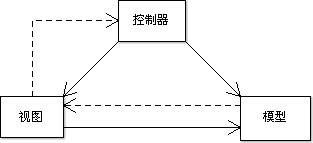
\includegraphics[scale=0.4]{ModelViewControllerDiagram.png}
\caption{MVC设计模式}
\end{figure}

在最初的JSP网页中,数据库查询语句等数据层代码是和HTML表示层代码混杂在一起的,虽然可以将数据从表示层分离开来,但是这样的良好设计通常并不是很容易做到的。

MVC可以从根本上强制性地将数据层和表示层代码分开,尽管构造MVC应用程序需要一些额外的工作,但是MVC带来的好处是毋庸置疑的。

MVC模式的目的是实现一种动态的程序设计,使后续对程序的修改和扩展简化,并且使程序某一部分的重复利用成为可能。

首先,多个 View 能共享一个 Model,这样同一个Web应用程序会提供多种用户界面。例如,用户希望既能够通过浏览器来收发电子邮件,还希望通过手机来访问电子邮箱,因此要求Web网站同时能提供Internet界面和WAP界面。

在MVC设计模式中, Model 响应用户请求并返回响应数据,View 负责格式化数据并把它们呈现给用户,业务逻辑和表示层分离,同一个 Model 可以被不同的 View 重用的做法提高了代码的可重用性。

其次,Controller 是自包含(self-contained)的高独立内聚的对象,与 Model 和 View 保持相对独立,所以可以方便的改变应用程序的数据层和业务规则。例如,把数据库从MySQL移植到Oracle,或者把RDBMS数据源改变成LDAP数据源,只需改变 Model 即可。

Controller 提高了应用程序的灵活性和可配置性。例如,Controller 可以用来连接不同的 Model 和 View 去完成用户的需求,也可以为构造应用程序提供强有力的手段,开发者给定一些可重用的 Model 、 View 和Controller就可以根据用户的需求选择适当的 Model 进行处理,然后选择适当的的 View 将处理结果显示给用户。

在正确地实现了控制器之后,不管数据来自数据库还是LDAP服务器,View 都会正确地显示它们。

除此之外,MVC模式通过对复杂度的简化,使程序结构更加直观,而且软件系统通过对自身基本部分分离的同时也赋予了各个基本部分应有的功能。例如,开发者可以通过自身的专长分组:

\begin{compactitem}
\item 控制器(Controller)- 负责对请求进行处理并转发请求。
\item 视图(View) - 图形界面设计。
\item 模型(Model) - 算法实现、数据管理和数据库设计等具体的功能。
\end{compactitem}

MVC将应用程序划分为三种组件后,开发者就可以设计并定义它们之间的相互作用,因此MVC模式的三个模块是相互独立的,改变其中一个不会影响其他两个,所以依据这种设计思想能构造出良好的少互扰性的构件。

在概念上,MVC模式强调 Model, View, Controller 的分离,各个模块也遵循着由 Controller 来处理消息,Model 掌管数据源,View 负责数据显示的职责分离原则,因此MVC 模式的 Framework在实现上通常会将 MVC 三个部分分离实现:

\begin{compactitem}
\item Model 负责数据访问,现代的 Framework 都会建议使用独立的数据对象 (DTO, POCO, POJO 等) 来替代弱类型的集合对象。

数据访问的代码会使用 Data Access Object或是 ORM-based Framework,也可以进一步使用 Repository Pattern 与 Unit of Works Pattern 来切割数据源的依赖性。

\item Controller 负责处理消息,较高级的 Framework 会有一个默认的实现(例如Spring 的 DispatcherServlet 或是 ASP.NET MVC 的 Controller 等)来作为 Controller 的基础。

在职责分离原则的基础上,每个 Controller 负责的部分不同,因此会将各个 Controller 切割成不同的文件以利于维护。

\item View 负责显示数据,这个部分多为前端应用,而 Controller 会有一个机制将处理的结果 (可能是 Model、集合或状态等) 交给 View,然后由 View 来决定怎么显示。例如 Spring Framework 使用 JSP 或相应技术,ASP.NET MVC 则使用 Razor 处理数据的显示。


\end{compactitem}


MVC 模式强调职责分离会产生很多文件,需要IDE基于类别对象的信息来组织代码编辑,而且 MVC 模式会要求开发者进一步思考应用程序的架构,而非用大杂烩的方式开发应用程序,对于应用程序的生命周期以及后续的可扩充与可维护性而言有相当正面的帮助。

MVC 职责分离也带来了一个现代软件工程要求的重要特性—可测试性 (Testability),基于MVC的应用程序在良好的职责分离的设计下,各个部分都可以独立进行单元测试,因此有利于与企业内的自动化测试、持续集成与持续发布流程的集成,减少应用程序改版部署所需的时间。

MVC 模式的应用程序的目的就是希望打破以往应用程序使用的大杂烩程序开发方式,并间接促使开发人员以更高的架构导向思维来思考应用程序的设计,因此MVC(或是其他的设计模式)都是有助于应用程序长远的发展,大杂烩式的程序在可扩充性和可维护性 (尤其是可测试性) 上远比 MVC 复杂很多。

MVC 模式的应用程序是在初始开发时期必须先思考并使用软件架构,结果就是可扩充性、可维护性和可测试性会因为 MVC 的特性而变得容易。

下面的示例使用JavaScript实现了一个基础的完整MVC示例。

\begin{lstlisting}[language=JavaScript]
/** 模拟Model,View和Controller **/
var M = {}, V = {}, C = {};

/** Model负责存储数据 **/
M.data = "Hello world.";

/** View负责把数据输出到网页上 **/
V.ender = (M) => {alert(M.data)};

/** Controller是Model和View的桥梁 **/
C.handleOnload = () => { V.render(M); }

/** 在网页读取时调用Controller **/
window.onload = C.handleOnload;
\end{lstlisting}

MFC Document/View架构是早期对于MVC模式的实现,MFC将程序分成CView以及CDocument两大类别,其中的Document对应MVC中的 Model ,View 相当于MVC中的 View+Controller,再加上CWinApp类别,合成三大项。


Java EE除了直接以Servlet来编写Controller之外,也可以使用Struts2或Spring Framework等,Model 则是由一个实体Bean来实现,视图(View)可能由JSP来实现。

Java Swing是一个标准的MVC架构,其中ComponentUI代表 View,负责渲染组件,Model 层包括JTextField的Document、JTable的TableModel和JTree的TreeModel等,Event机制可以看作是Controller。

Ruby on Rails的Model 部分使用 Active Record 概念实现,并使用Migration机制来控制Model的结构。

JavaScript的Backbone.js、Angular.js和Ember.js都实现了MVC模式。

PHP的Yaf、CakePHP、CodeIgniter、Symfony、Yii、Phalcon、Laravel和Zend Framework都是MVC框架。


\section{Controller}

控制器(Controller)可以在不同层面间发挥组织作用,从而控制应用程序的流程。

Controller处理事件并作出响应,这里的“事件”包括用户的行为和数据 Model 上的改变等。



Yaf默认的控制器为controllers/Index.php,其内容如下:

\begin{lstlisting}[language=PHP]
<?php
class IndexController extends Yaf_Controller_Abstract {
    /* default action name */
    public function indexAction() {
        $this->_view->word = "hello world, yaf";
        // or
        // $this->getView()->content = "hello world, yaf";
    }
}
\end{lstlisting}

\section{Model}

模型(Model) 用于封装与应用程序的业务逻辑相关的数据以及对数据的处理方法。

“Model”有对数据直接访问的权力(例如对数据库的访问),而且“Model”不依赖“View”和“Controller”。

也就是说, Model 不关心它会被如何显示或是如何被操作,但是 Model 中数据的变化一般会通过一种刷新机制被公布。为了实现这种机制,那些用于监视此 Model 的 View 必须事先在此 Model 上注册,从而View就可以了解在数据 Model 上发生的改变。




\section{View}

虽然理论上并不是必需的,但是视图(View)能够实现数据有目的的显示。

在 View 中一般不包含程序上的逻辑,因此为了实现 View 上的数据刷新功能,View 需要访问它监视的数据模型(Model),应该事先在被它监视的数据那里注册。




Yaf默认的视图文件为application/views/index/index.phtml,Yaf提供了一个默认的模板引擎——Yaf\_View\_Simple来支持使用PHP编码的视图模板。

\begin{lstlisting}[language=HTML]
<html>
  <head>
    <title>Hello world</title>
  </head>
  <body>
     <?php echo $content; ?>
  </body>
</html>
\end{lstlisting}

运行上述的Yaf示例应用程序的输出类似于:


\begin{lstlisting}[language=bash]
<html>
  <head>
    <title>Hello world</title>
  </head>
  <body>
     hello world, yaf
  </body>
</html>
\end{lstlisting}


\chapter{Yaf\_Application}

Yaf\_Application为应用提供了一个辅助设施。

Yaf\_Application提供了可重用的资源、常见的和模块化的引导类以及依赖检查。

和Yii框架的CApplication类一样,Yaf的Yaf\_Application类也实现了单例模式,而且Yaf\_Application不能被序列化和反序列化, 否则当尝试使用PHPUnit来为Yaf写一些测试用例的时候会造成一些不必要的麻烦。

开发者可以使用PHPUnit的@backupGlobals注释来控制全局变量的备份和恢复操作, 从而可以解决上述这个问题。




\begin{lstlisting}[language=PHP]
final Yaf_Application {
  /* 属性 */
  protected $config ;
  protected $dispatcher ;
  protected static $_app ;
  protected $_modules ;
  protected $_running ;
  protected $_environ ;
  /* 方法 */
  public static void app ( void )
  public void bootstrap ([ Yaf_Bootstrap_Abstract $bootstrap ] )
  public Yaf_Application clearLastError ( void )
  private void __clone ( void )
  public __construct ( mixed $config [, string $envrion ] )
  public void __destruct ( void )
  public void environ ( void )
  public void execute ( callable $entry , string $... )
  public Yaf_Application getAppDirectory ( void )
  public Yaf_Config_Abstract getConfig ( void )
  public Yaf_Dispatcher getDispatcher ( void )
  public string getLastErrorMsg ( void )
  public int getLastErrorNo ( void )
  public array getModules ( void )
  public void run ( void )
  public Yaf_Application setAppDirectory ( string $directory )
  private void __sleep ( void )
  private void __wakeup ( void )
}
\end{lstlisting}

\section{Property}


\subsection{\$config}
\subsection{\$dispatcher}
\subsection{\$\_app}
\subsection{\$\_modules}
\subsection{\$\_running}
\subsection{\$\_environ}

\section{Method}


\subsection{Yaf\_Application::app()}

Yaf\_Application::app()方法没有参数。

\begin{lstlisting}[language=PHP]
public static void Yaf_Application::app ( void )
\end{lstlisting}

返回值为当前的Yaf\_Application实例(一个单例模式的对象), 如果在调用之前没有初始化一个Yaf\_Application实例的话,它将返回NULL。

也可以使用Yaf\_Dispatcher::getApplication()来得到Yaf\_Application的实例。











\subsection{Yaf\_Application::bootstrap()}

调用bootstrap(),可以传入一个Yaf\_Bootstrap\_Abstract对象作为可选参数,并返回一个Yaf\_Application实例化对象。

\begin{lstlisting}[language=PHP]
public void Yaf_Application::bootstrap ([ Yaf_Bootstrap_Abstract $bootstrap ] )
\end{lstlisting}

具体来说,Yaf\_Application::bootstrap()方法会指示Yaf\_Application去寻找Bootstrap,并按照声明的顺序,执行所有在Bootstrap类中定义的以\_init开头的方法。 如果没有提供变量bootstrap,Yaf默认会去application.directory中寻找Bootstrap。

\begin{lstlisting}[language=PHP]
<?php
/**
 * This file should be under the APPLICATION_PATH . "/application/"
 * (which was defined in the config passed to Yaf_Application).
 * and named Bootstrap.php,  so the Yaf_Application can find it 
 */
class Bootstrap extends Yaf_Bootstrap_Abstract {
   function _initConfig(Yaf_Dispatcher $dispatcher) {
      echo "1st called\n";
   }
   function _initPlugin($dispatcher) {
      echo "2nd called\n";
   }
}
\end{lstlisting}

\begin{example}
Yaf\_Application::bootstrap()示例
\begin{lstlisting}[language=PHP]
defined('APPLICATION_PATH')  // APPLICATION_PATH will be used in the ini config file
   || define('APPLICATION_PATH', __DIR__); // __DIR__
$application = new Yaf_Application(APPLICATION_PATH.'/conf/application.ini');
$application->bootstrap();
// 以上例程的输出类似于:
1st called
2nd called
\end{lstlisting}
\end{example}


\begin{example}
Yaf\_Application::bootstrap()载入Session类和Database类
\begin{lstlisting}[language=PHP]
<?php
class Bootstrap extends Yaf_Bootstrap_Abstract 
{
   public function _initSession(Yaf_Dispatcher $dispatcher) {
       $session = new Vender\Session();
       $session->start();
   }
   public function _initDatabase(Yaf_Dispatcher $dispatcher) {
       $config = Yaf_Application::app()->getConfig()->application->database;
       Yaf_Registry::set('db', Vendor\Database($config));
   }
}
\end{lstlisting}
\end{example}

\subsection{Yaf\_Application::clearLastError()}

clearLastError()方法没有参数。

\begin{lstlisting}[language=PHP]
public Yaf_Application Yaf_Application::clearLastError ( void )
\end{lstlisting}

清除最后的错误信息,开发者可以自定义错误处理器。


\begin{lstlisting}[language=PHP]
<?php
function error_handler($errno,$errstr,$errfile,$errline) {
   Yaf_Application::app()->clearLastError();
   var_dump(Yaf_Application::app()->getLastErrorNo());
}
$config = array(
   "application"=>array(
      "directory"=>"/tmp/notexists",
      "dispatcher"=>array(
          // trigger error instead of throw exception when error occure
          "throwException"=>0,
      ),
   ),
);
$app = new Yaf_Application($config);
$app->getDispatcher()->setErrorHandler("error_handler",E_RECOVERABLE_ERROR);
$app->run();
// 以上例程的输出类似于:
// int(0)
\end{lstlisting}





\subsection{Yaf\_Application::\_\_clone()}

Yaf\_Application类不允许被克隆,而且\_\_clone()函数没有参数。






\begin{lstlisting}[language=PHP]
private void Yaf_Application::__clone ( void )
\end{lstlisting}





\subsection{Yaf\_Application::\_\_construct()}

构造函数可以初始化一个 Yaf\_Application。




\begin{lstlisting}[language=PHP]
publicYaf_Application::__construct ( mixed $config [, string $envrion ] )
\end{lstlisting}

\begin{compactitem}
\item \$config包含关联数组的配置, 或者一个指向ini格式的配置文件的路径的字符串。
\item \$environ则指示应该载入product还是dev段的配置信息。
\end{compactitem}




如果是一个ini配置文件,那么配置文件中应该有一个定义了yaf.environ 的配置节,这个在生产环境中是默认的。

如果使用了ini配置文件作为应用配置的容器,需要打开yaf.cache\_config 来提升性能。

\begin{lstlisting}[language=PHP]
[product]
;this one should alway be defined, and have no default value
application.directory=APPLICATION_PATH

;following configs have default value, you may no need to define them
application.library = APPLICATION_PATH . "/library"
application.dispatcher.throwException=1
application.dispatcher.catchException=1

application.baseUri=""

;the php script ext name
ap.ext=php

;the view template ext name
ap.view.ext=phtml

ap.dispatcher.defaultModuel=Index
ap.dispatcher.defaultController=Index
ap.dispatcher.defaultAction=index

;defined modules
ap.modules=Index
\end{lstlisting}


\begin{lstlisting}[language=PHP]
<?php
defined('APPLICATION_PATH')                  // APPLICATION_PATH will be used in the ini config file
    || define('APPLICATION_PATH', __DIR__)); //__DIR__ 

$application = new Yaf_Application(APPLICATION_PATH.'/conf/application.ini');
$application->bootstrap()->run();
\end{lstlisting}

向Yaf\_Application传入的配置也可以是一个数组,例如:

\begin{lstlisting}[language=PHP]
<?php
$config = array(
    "application" => array(
        "directory" => realpath(dirname(__FILE__)) . "/application",
    ),
);

/** Yaf_Application */
$application = new Yaf_Application($config);
$application->bootstrap()->run();
\end{lstlisting}



\begin{lstlisting}[language=PHP]

\end{lstlisting}


\subsection{Yaf\_Application::\_\_destruct()}

析构函数(没有参数)






\begin{lstlisting}[language=PHP]
public void Yaf_Application::__destruct ( void )
\end{lstlisting}



\begin{lstlisting}[language=PHP]

\end{lstlisting}



\begin{lstlisting}[language=PHP]

\end{lstlisting}


\subsection{Yaf\_Application::environ()}

获取当前Yaf\_Application的环境名(例如product或dev),它被定义在yaf.environ,默认为product。






\begin{lstlisting}[language=PHP]
public void Yaf_Application::environ ( void )
\end{lstlisting}

environ()方法没有参数。

\begin{lstlisting}[language=PHP]
<?php
$config = array(
    "application" => array(
        "directory" => realpath(dirname(__FILE__)) . "/application",
    ),
);

/** Yaf_Application */
$application = new Yaf_Application($config);
print_r($application->environ());
// 以上例程的输出类似于:
// product
\end{lstlisting}



\begin{lstlisting}[language=PHP]

\end{lstlisting}


\subsection{Yaf\_Application::execute()}

运行回调函数






\begin{lstlisting}[language=PHP]
public void Yaf_Application::execute ( callable $entry , string $... )
\end{lstlisting}

execute()方法通常用于在cron任务中运行Yaf\_Application,而且在cron任务中也可以使用autoloader和Bootstrap机制。

\begin{compactitem}
\item \$entry是一个有效的回调函数
\item \texttt{\$...}是零个或多个要传递给函数的参数
\end{compactitem}



\begin{lstlisting}[language=PHP]
<?php
function main($argc,$argv) {

}
$config = array(
    "application" => array(
        "directory" => realpath(dirname(__FILE__)) . "/application",
    ),
);
/* Yaf_Application */
$application = new Yaf_Application($config);
$application->execute("main", $argc,  $argv);
\end{lstlisting}



\begin{lstlisting}[language=PHP]

\end{lstlisting}


\subsection{Yaf\_Application::getAppDirectory()}

获取Yaf应用程序所在的目录






\begin{lstlisting}[language=PHP]
public Yaf_Application Yaf_Application::getAppDirectory ( void )
\end{lstlisting}



\begin{lstlisting}[language=PHP]

\end{lstlisting}



\begin{lstlisting}[language=PHP]

\end{lstlisting}


\subsection{Yaf\_Application::getConfig()}

获取Yaf\_Config\_Abstract的实例。






\begin{lstlisting}[language=PHP]
public Yaf_Config_Abstract Yaf_Application::getConfig ( void )
\end{lstlisting}

getConfig()方法没有参数,返回值是一个Yaf\_Config\_Abstract类的实例。

\begin{lstlisting}[language=PHP]
<?php
$config = array(
    "application" => array(
        "directory" => realpath(dirname(__FILE__)) . "/application",
    ),
);

/** Yaf_Application */
$application = new Yaf_Application($config);
print_r($application->getConfig());
// 以上例程的输出类似于:
// Yaf_Config_Simple Object
// (
//    [_config:protected] => Array
//        (
//            [application] => Array
//                (
//                    [directory] => /home/laruence/local/www/htdocs/application
//                )
//
//        )
//
//    [_readonly:protected] => 1
// )
\end{lstlisting}






\subsection{Yaf\_Application::getDispatcher()}

获取Yaf\_Dispatcher的实例。



\begin{lstlisting}[language=PHP]
public Yaf_Dispatcher Yaf_Application::getDispatcher ( void )
\end{lstlisting}


\begin{lstlisting}[language=PHP]
<?php
$config = array(
    "application" => array(
        "directory" => realpath(dirname(__FILE__)) . "/application",
    ),
);

/** Yaf_Application */
$application = new Yaf_Application($config);
print_r($application->getDispatcher());
// 以上例程的输出类似于:
// Yaf_Dispatcher Object
// (
//     [_router:protected] => Yaf_Router Object
//         (
//             [_routes:protected] => Array
//                 (
//                     [_default] => Yaf_Route_Static Object
//                         (
//                         )
//                 )
//             [_current:protected] => 
//         )
//     [_view:protected] => 
//     [_request:protected] => Yaf_Request_Http Object
//         (
//             [module] => 
//             [controller] => 
//             [action] => 
//             [method] => Cli
//             [params:protected] => Array
//                 (
//                 )
//             [language:protected] => 
//             [_exception:protected] => 
//             [_base_uri:protected] => 
//             [uri:protected] => 
//             [dispatched:protected] => 
//             [routed:protected] => 
//         )
//     [_plugins:protected] => Array
//         (
//         )
//     [_auto_render:protected] => 1
//     [_return_response:protected] => 
//     [_instantly_flush:protected] => 
//     [_default_module:protected] => Index
//     [_default_controller:protected] => Index
//     [_default_action:protected] => index
//     [_response] => Yaf_Response_Cli Object
//         (
//             [_header:protected] => Array
//                 (
//                 )
//             [_body:protected] => 
//             [_sendheader:protected] => 
//         )
// )
\end{lstlisting}



\subsection{Yaf\_Application::getLastErrorMsg()}

获取最近产生的错误的错误信息。






\begin{lstlisting}[language=PHP]
public string Yaf_Application::getLastErrorMsg ( void )
\end{lstlisting}

\begin{example}
getLstErrorMsg()示例
\begin{lstlisting}[language=PHP]
<?php
function error_handler($errno, $errstr, $errfile, $errline) {
   var_dump(Yaf_Application::app()->getLastErrorMsg());
}

$config = array(                   
 "application" => array(
   "directory" => "/tmp/notexists",
     "dispatcher" => array(
       "throwException" => 0, //trigger error instead of throw exception when error occure
      ),
  ),
);

$app = new Yaf_Application($config);
$app->getDispatcher()->setErrorHandler("error_handler", E_RECOVERABLE_ERROR);
$app->run();
// 以上例程的输出类似于:
// string(69) "Could not find controller script /tmp/notexists/controllers/Index.php"
\end{lstlisting}
\end{example}


\begin{lstlisting}[language=PHP]

\end{lstlisting}


\subsection{Yaf\_Application::getLastErrorNo()}

获取最近产生的错误的错误代码。






\begin{lstlisting}[language=PHP]
public int Yaf_Application::getLastErrorNo ( void )
\end{lstlisting}


\begin{example}
getLstErrorNo()示例
\begin{lstlisting}[language=PHP]
<?php
function error_handler($errno, $errstr, $errfile, $errline) {
   var_dump(Yaf_Application::app()->getLastErrorNo());
   var_dump(Yaf_Application::app()->getLastErrorNo() == YAF_ERR_NOTFOUND_CONTROLLER);
}

$config = array(
  "application" => array(
   "directory" => "/tmp/notexists",
     "dispatcher" => array(
       "throwException" => 0, //trigger error instead of throw exception when error occure
      ),
  ),
);

$app = new Yaf_Application($config);
$app->getDispatcher()->setErrorHandler("error_handler", E_RECOVERABLE_ERROR);
$app->run();
// 以上例程的输出类似于:
// int(516)
// bool(true)
\end{lstlisting}
\end{example}





\subsection{Yaf\_Application::getModules()}

获取在配置文件中声明的模块,如果没有声明,它的默认值将是``Index"。





\begin{lstlisting}[language=PHP]
public array Yaf_Application::getModules ( void )
\end{lstlisting}

\begin{lstlisting}[language=PHP]
<?php
$config = array(
    "application" => array(
        "directory" => realpath(dirname(__FILE__)) . "/application",
    ),
);

/** Yaf_Application */
$application = new Yaf_Application($config);
print_r($application->getModules());
// 以上例程的输出类似于:
// Array
// (
//     [0] => Index
// )
\end{lstlisting}


\subsection{Yaf\_Application::run()}

运行Yaf\_Application(),run()方法本身没有参数。





\begin{lstlisting}[language=PHP]
public void Yaf_Application::run ( void )
\end{lstlisting}

具体来说,run()方法运行一个Yaf\_Application,开始接受并处理请求、分发路由并做出相应的响应,最终将响应返回给客户端。




\subsection{Yaf\_Application::setAppDirectory()}

改变Yaf应用程序的目录到指定的目录。






\begin{lstlisting}[language=PHP]
public Yaf_Application Yaf_Application::setAppDirectory ( string $directory )
\end{lstlisting}



\begin{lstlisting}[language=PHP]

\end{lstlisting}



\begin{lstlisting}[language=PHP]

\end{lstlisting}


\subsection{Yaf\_Application::\_\_sleep()}

Yaf\_Application不能被序列化。






\begin{lstlisting}[language=PHP]
private void Yaf_Application::__sleep ( void )
\end{lstlisting}



\subsection{Yaf\_Application::\_\_wakeup()}

Yaf\_Application不能被反序列化。







\begin{lstlisting}[language=PHP]
private void Yaf_Application::__wakeup ( void )
\end{lstlisting}

\chapter{Yaf\_Bootstrap\_Abstract}

Bootstrap是用来在Application运行(run)之前做一些初始化工作的机制,开发者可以通过继承Yaf\_Bootstrap\_Abstract 来定义自己的Bootstrap类。

在Bootstrap类中所有以``\_init"开头的公有的方法,都会被按照定义顺序依次在Yaf\_Application::bootstrap()方法被调用的时刻进行调用和执行。



\begin{lstlisting}[language=PHP]
<?php
class Bootstrap extends Yaf_Bootstrap_Abstract {
   public function _initConfig(Yaf_Dispatcher $dispatcher) {
       var_dump(__METHOD__);
   }
   public function _initPlugin(Yaf_Dispatcher $dispatcher) {
       var_dump(__METHOD__);
   }
}
$config = array(
   "application"=>array(
       "directory"=>dirname(__FILE__)."/application";
   ),
);
$app=new Yaf_Application($config);
$app->bootstrap();

// 以上例程的输出类似于:
// string(22) "Bootstrap::_initConfig"
// string(22) "Bootstrap::_initPlugin"
\end{lstlisting}





\chapter{Yaf\_Dispatcher}

Yaf\_Dispatcher用于初始化处理请求的运行环境。

具体来说,Yaf\_Dispatcher类协调路由来的请求,并分发和执行发现的动作,然后收集动作产生的响应,输出响应给请求者,并在整个过程完成以后返回响应。

Yaf\_Dispatcher是单例模式运行的,也就是说自始至终只生成一个Yaf\_Dispatcher实例,因此可以把它看成是在分发过程中生成的对象的注册表,可以从中获取到分发过程中产生的对象。



\begin{lstlisting}[language=PHP]
final Yaf_Dispatcher {
  /* 属性 */
  protected $_router ;
  protected $_view ;
  protected $_request ;
  protected $_plugins ;
  protected static $_instance ;
  protected $_auto_render ;
  protected $_return_response ;
  protected $_instantly_flush ;
  protected $_default_module ;
  protected $_default_controller ;
  protected $_default_action ;
  /* 方法 */
  public Yaf_Dispatcher autoRender ( bool $flag )
  public Yaf_Dispatcher catchException ([ bool $flag ] )
  private void __clone ( void )
  public__construct ( void )
  public bool disableView ( void )
  public Yaf_Response_Abstract dispatch ( Yaf_Request_Abstract $request )
  public Yaf_Dispatcher enableView ( void )
  public Yaf_Dispatcher flushInstantly ( bool $flag )
  public Yaf_Application getApplication ( void )
  public static Yaf_Dispatcher getInstance ( void )
  public Yaf_Request_Abstract getRequest ( void )
  public Yaf_Router getRouter ( void )
  public Yaf_View_Interface initView ( string $templates_dir [, array $options ] )
  public Yaf_Dispatcher registerPlugin ( Yaf_Plugin_Abstract $plugin )
  public Yaf_Dispatcher returnResponse ( bool $flag )
  public Yaf_Dispatcher setDefaultAction ( string $action )
  public Yaf_Dispatcher setDefaultController ( string $controller )
  public Yaf_Dispatcher setDefaultModule ( string $module )
  public Yaf_Dispatcher setErrorHandler ( call $callback , int $error_types )
  public Yaf_Dispatcher setRequest ( Yaf_Request_Abstract $request )
  public Yaf_Dispatcher setView ( Yaf_View_Interface $view )
  private void __sleep ( void )
  public Yaf_Dispatcher throwException ([ bool $flag ] )
  private void __wakeup ( void )
}
\end{lstlisting}



\section{Property}





\subsection{\$\_router}

\subsection{\$\_view}
\subsection{\$\_request}
\subsection{\$\_plugins}
\subsection{\$\_instance}
\subsection{\$\_auto\_render}
\subsection{\$\_return\_response}
\subsection{\$\_instantly\_flush}
\subsection{\$\_default\_module}
\subsection{\$\_default\_controller}
\subsection{\$\_default\_action}





\begin{lstlisting}[language=PHP]

\end{lstlisting}



\begin{lstlisting}[language=PHP]

\end{lstlisting}





\begin{lstlisting}[language=PHP]

\end{lstlisting}




\begin{lstlisting}[language=PHP]

\end{lstlisting}



\begin{lstlisting}[language=PHP]

\end{lstlisting}




\begin{lstlisting}[language=PHP]

\end{lstlisting}





\begin{lstlisting}[language=PHP]

\end{lstlisting}




\begin{lstlisting}[language=PHP]

\end{lstlisting}



\begin{lstlisting}[language=PHP]

\end{lstlisting}



\begin{lstlisting}[language=PHP]

\end{lstlisting}














\begin{lstlisting}[language=PHP]

\end{lstlisting}



\begin{lstlisting}[language=PHP]

\end{lstlisting}



\begin{lstlisting}[language=PHP]

\end{lstlisting}

\section{Method}


\subsection{Yaf\_Dispatcher::autoRender()}

开启/关闭自动渲染功能(接受bool型参数)

\begin{lstlisting}[language=PHP]
public Yaf_Dispatcher Yaf_Dispatcher::autoRender ( bool $flag )
\end{lstlisting}

Yaf默认开启自动渲染功能,在开启的情况下,action执行完成以后,Yaf\_Dispatcher 会自动调用view引擎去渲染该action对应的视图模板。 

开发者也可以通过调用这个函数并将 flag 参数的值设为TRUE来进行人工干预。例如,可以在一个action中仅返回FALSE来阻止当前action对应视图的自动渲染。


\begin{lstlisting}[language=PHP]
<?php
class IndexController extends Yaf_Controller_Abstract {
    /* init method will be called as soon as a controller is initialized */ 
    public function init() {
         if($this->getRequest()->isXMLHttpResquest()) {
             //do not call render for ajax request
             //we will outpu a json string
             Yaf_Dispatcher::getInstance()->autoRender(FLASE);
         }
    }
}
\end{lstlisting}



\begin{lstlisting}[language=PHP]

\end{lstlisting}

\subsection{Yaf\_Dispatcher::catchException()}

开启/关闭自动异常捕获功能(接受bool型参数)


\begin{lstlisting}[language=PHP]
public Yaf_Dispatcher Yaf_Dispatcher::catchException ([ bool $flag ] )
\end{lstlisting}

当 application.dispatcher.throwException 开启的时候(也可以通过调用 Yaf\_Dispatcher::throwException(TRUE)() 来开启它),Yaf将会抛出异常而不是触发异常发生。

如果开启了 Yaf\_Dispatcher::catchException() (可以通过设置application.dispatcher.catchException来开启),并且在定义了异常处理的controller的情况下,Yaf会将所有未捕获的异常交给Error Controller的Error Action来处理。例如,捕获异常后可以根据异常代码来渲染指定的异常页面并显示给用户。

\begin{lstlisting}[language=PHP]
<?php
class ErrorController extends Yaf_Controller_Abstract {
    public function init() {}
    /** 
      * you can also call to Yaf_Request_Abstract::getException to  
      * get the un-caught exception.
      */
    public function error($exception) {
        // error occurs
        switch ($exception->getCode()) {
            case YAF_ERR_NOTFOUND_MODULE:
            case YAF_ERR_NOTFOUND_CONTROLLER:
            case YAF_ERR_NOTFOUND_ACTION:
            case YAF_ERR_NOTFOUND_VIEW:
                echo 404, ":",$exception->getMessage();
                break;
            default:
                $message=$exception->getMessage();
                echo 0,":",$exception->getMessage();
                break;
        }
    }
}
// 以上例程的输出类似于:
/* now if some error occur, assuming access a non-exists controller
 * (or you can throw a exception yourself): 
 */
404:Could not find controller script **/application/controllers/No-exists-controller.php
\end{lstlisting}



\subsection{Yaf\_Dispatcher::\_\_clone()}

 Yaf\_Dispatcher 不能被克隆


\begin{lstlisting}[language=PHP]
private void Yaf_Dispatcher::__clone ( void )
\end{lstlisting}




\subsection{Yaf\_Dispatcher::\_\_construct()}

Yaf\_Dispatcher 构造函数

\begin{lstlisting}[language=PHP]
publicYaf_Dispatcher::__construct ( void )
\end{lstlisting}



\subsection{Yaf\_Dispatcher::disableView()}

关闭自动渲染


\begin{lstlisting}[language=PHP]
public bool Yaf_Dispatcher::disableView ( void )
\end{lstlisting}

在一些用户自己会输出信息的情况下使用关闭自动渲染。例如,可以在一个action中仅仅返回FALSE来阻止当前action对应视图的自动渲染。


\subsection{Yaf\_Dispatcher::dispatch()}

分发请求


\begin{lstlisting}[language=PHP]
public Yaf_Response_Abstract Yaf_Dispatcher::dispatch ( Yaf_Request_Abstract $request )
\end{lstlisting}

Yaf\_Dispatcher 的dispatch()方法的工作非常繁重,而且它还需要一个request对象。

分发请求的过程有三个不同的事件:

\begin{compactitem}
\item 路由
\item 分发
\item 响应
\end{compactitem}

路由只发生一次,当dispatch()被调用的时候,需要使用请求对象中的值(例如PATH\_INFO)。

分发发生在一个循环中,一个请求可能会分发出多个action, 或者controller或者一个plugin可能重置请求对象来强制分发其他的action。 

当所有分发的步骤都执行完毕,Yaf\_Dispatcher 会返回一个响应,因此如果中途出错,可以执行exit()来直接返回输出,其他未指定的操作就不需要再继续执行。





\subsection{Yaf\_Dispatcher::enableView()}

开启自动渲染


\begin{lstlisting}[language=PHP]
public Yaf_Dispatcher Yaf_Dispatcher::enableView ( void )
\end{lstlisting}

如果前面的步骤禁用了自动渲染,在后面的步骤中还可以通过调用enableView()方法来重新开启自动渲染。

\begin{lstlisting}[language=PHP]

\end{lstlisting}
\subsection{Yaf\_Dispatcher::flushInstantly()}

打开关闭自动响应

\begin{lstlisting}[language=PHP]
public Yaf_Dispatcher Yaf_Dispatcher::flushInstantly ( bool $flag )
\end{lstlisting}


\subsection{Yaf\_Dispatcher::getApplication()}

和Yaf\_Application::app()的执行结果相同,二者都是获取当前的Yaf\_Application实例。


\begin{lstlisting}[language=PHP]
public Yaf_Application Yaf_Dispatcher::getApplication ( void )
\end{lstlisting}






\subsection{Yaf\_Dispatcher::getInstance()}


获取当前的Yaf\_Dispatcher实例

\begin{lstlisting}[language=PHP]
public static Yaf_Dispatcher Yaf_Dispatcher::getInstance ( void )
\end{lstlisting}



\subsection{Yaf\_Dispatcher::getRequest()}


获取当前的请求实例

\begin{lstlisting}[language=PHP]
public Yaf_Request_Abstract Yaf_Dispatcher::getRequest ( void )
\end{lstlisting}





\subsection{Yaf\_Dispatcher::getRouter()}

获取路由器


\begin{lstlisting}[language=PHP]
public Yaf_Router Yaf_Dispatcher::getRouter ( void )
\end{lstlisting}





\subsection{Yaf\_Dispatcher::initView()}

初始化视图引擎并返回它


\begin{lstlisting}[language=PHP]
public Yaf_View_Interface Yaf_Dispatcher::initView ( string $templates_dir [, array $options ] )
\end{lstlisting}

在初始化视图引擎时可以传入视图模板的目录,以及可选参数。



\subsection{Yaf\_Dispatcher::registerPlugin()}


注册一个插件


\begin{lstlisting}[language=PHP]
public Yaf_Dispatcher Yaf_Dispatcher::registerPlugin ( Yaf_Plugin_Abstract $plugin )
\end{lstlisting}


\begin{lstlisting}[language=PHP]
<?php
class Bootstrap extends Yaf_Bootstrap_Abstract {
   public function _initPlugin(Yaf_Dispatcher $dispatcher) {
        /**
         * Yaf assumes plugin scripts under [application.directory] .  "/plugins" 
         * for this case, it will be:
         * [application.directory] . "/plugins/" . "User" . [application.ext]
         */ 
        $user=new UserPlugin();
        $dispatcher->registerPlugin($user);
   }
}
\end{lstlisting}

Yaf假设插件脚本位于plugins目录下。




\subsection{Yaf\_Dispatcher::returnResponse()}

是否返回响应。

\begin{lstlisting}[language=PHP]
public Yaf_Dispatcher Yaf_Dispatcher::returnResponse ( bool $flag )
\end{lstlisting}

\subsection{Yaf\_Dispatcher::setDefaultAction()}

设置路由的默认动作(传入指定的Action名字)

\begin{lstlisting}[language=PHP]
public Yaf_Dispatcher Yaf_Dispatcher::setDefaultAction ( string $action )
\end{lstlisting}


\subsection{Yaf\_Dispatcher::setDefaultController()}

设置路由的默认控制器(传入指定的控制器名字)

\begin{lstlisting}[language=PHP]
public Yaf_Dispatcher Yaf_Dispatcher::setDefaultController ( string $controller )
\end{lstlisting}

\subsection{Yaf\_Dispatcher::setDefaultModule()}

设置路由的默认模块(传入指定的模块名字)

\begin{lstlisting}[language=PHP]
public Yaf_Dispatcher Yaf_Dispatcher::setDefaultModule ( string $module )
\end{lstlisting}

\subsection{Yaf\_Dispatcher::setErrorHandler()}

设置错误处理函数。例如,如果在application.dispatcher.throwException关闭的情况下,Yaf会在出错的时候触发错误,这个时候如果设置了错误处理函数,则会把控制交给错误处理函数处理,因此当错误发生的时候这个错误处理函数将被调用。

\begin{compactitem}
\item \$callback:错误处理的回调函数
\item \$error\_type:错误类型
\end{compactitem}



\begin{lstlisting}[language=PHP]
<?php
$dispatcher->setErrorHandler(array(get_class($this),'error_handler'));
\end{lstlisting}


\subsection{Yaf\_Dispatcher::setRequest()}

设置请求

\begin{lstlisting}[language=PHP]
public Yaf_Dispatcher Yaf_Dispatcher::setRequest ( Yaf_Request_Abstract $request )
\end{lstlisting}


\subsection{Yaf\_Dispatcher::setView()}

设置视图引擎(默认传入Yaf\_View\_Interface的实例)

\begin{lstlisting}[language=PHP]
public Yaf_Dispatcher Yaf_Dispatcher::setView ( Yaf_View_Interface $view )
\end{lstlisting}

Yaf提供了一个试图引擎——Yaf\_View\_Simple,如果需要使用自定义的视图引擎代替 Yaf\_View\_Simple , 这个函数可以解决这个问题。


\begin{example}
使用Smarty代替默认的视图引擎
\begin{lstlisting}[language=PHP]
<?php
require "/path/to/smarty/Smarty.class.php";

class Smarty_Adapter implements Yaf_View_Interface
{
    /**
     * Smarty object
     * @var Smarty
     */
    public $_smarty;
 
    /**
     * Constructor
     *
     * @param string $tmplPath
     * @param array $extraParams
     * @return void
     */
    public function __construct($tmplPath = null, $extraParams = array()) {
        $this->_smarty = new Smarty;
 
        if (null !== $tmplPath) {
            $this->setScriptPath($tmplPath);
        }
 
        foreach ($extraParams as $key => $value) {
            $this->_smarty->$key = $value;
        }
    }
 
    /**
     * Set the path to the templates
     *
     * @param string $path The directory to set as the path.
     * @return void
     */
    public function setScriptPath($path)
    {
        if (is_readable($path)) {
            $this->_smarty->template_dir = $path;
            return;
        }
 
        throw new Exception('Invalid path provided');
    }
 
    /**
     * Assign a variable to the template
     *
     * @param string $key The variable name.
     * @param mixed $val The variable value.
     * @return void
     */
    public function __set($key, $val)
    {
        $this->_smarty->assign($key, $val);
    }
 
    /**
     * Allows testing with empty() and isset() to work
     *
     * @param string $key
     * @return boolean
     */
    public function __isset($key)
    {
        return (null !== $this->_smarty->get_template_vars($key));
    }
 
    /**
     * Allows unset() on object properties to work
     *
     * @param string $key
     * @return void
     */
    public function __unset($key)
    {
        $this->_smarty->clear_assign($key);
    }
 
    /**
     * Assign variables to the template
     *
     * Allows setting a specific key to the specified value, OR passing
     * an array of key => value pairs to set en masse.
     *
     * @see __set()
     * @param string|array $spec The assignment strategy to use (key or
     * array of key => value pairs)
     * @param mixed $value (Optional) If assigning a named variable,
     * use this as the value.
     * @return void
     */
    public function assign($spec, $value = null) {
        if (is_array($spec)) {
            $this->_smarty->assign($spec);
            return;
        }
 
        $this->_smarty->assign($spec, $value);
    }
 
    /**
     * Clear all assigned variables
     *
     * Clears all variables assigned to Yaf_View either via
     * {@link assign()} or property overloading
     * ({@link __get()}/{@link __set()}).
     *
     * @return void
     */
    public function clearVars() {
        $this->_smarty->clear_all_assign();
    }
 
    /**
     * Processes a template and returns the output.
     *
     * @param string $name The template to process.
     * @return string The output.
     */
    public function render($name, $value = NULL) {
        return $this->_smarty->fetch($name);
    }

    public function display($name, $value = NULL) {
        echo $this->_smarty->fetch($name);
    }
}
\end{lstlisting}
\end{example}

\begin{example}
使用Yaf\_Dispatcher::setView()设置视图渲染引擎
\begin{lstlisting}[language=PHP]
<?php
class Bootstrap extends Yaf_Bootstrap_Abstract {
    /**
     * there are some config for smarty in the config:
     *
     * smarty.left_delimiter   = "{{"
     * smarty.right_delimiter  = "}}"
     * smarty.template_dir     = APPLICATION_PATH "/views/scripts/"
     * smarty.compile_dir      = APPLICATION_PATH "/views/templates_c/"
     * smarty.cache_dir        = APPLICATION_PATH "/views/templates_d/"
     *
     */
    public function _initConfig() {
        $config = Yaf_Applicatin::app()->getConfig();
        Yaf_Registry::set('config',$config);
    }
    
    public function _initLocalName() {
        /** we put class Smarty_Adapter under the local library directory */
        Yaf\_Loader::getInstance()->registerLocalNamespace('Smarty');
    }
    
    public function _initSmarty(Yaf_Dispatcher $dispatcher) {
        $smarty = new Smarty_Adapter(null,Yaf_Registry::get('config')->get('smarty');
        $dispatcher->setView($smarty);
         /* now the Smarty view engine become the default view engine of Yaf */
    }
}
\end{lstlisting}
\end{example}

\subsection{Yaf\_Dispatcher::\_\_sleep()}

Yaf\_Dispatcher 不能被序列化

\begin{lstlisting}[language=PHP]
private void Yaf_Dispatcher::__sleep ( void )
\end{lstlisting}

\subsection{Yaf\_Dispatcher::throwException()}

开启/关闭异常抛出

\begin{lstlisting}[language=PHP]
public Yaf_Dispatcher Yaf_Dispatcher::throwException ([ bool $flag ] )
\end{lstlisting}

Yaf\_Dispatcher可以设置当意外的错误发生时是否开启/关闭异常抛出。其中,当开启的时候,Yaf将会抛出异常而不是触发可捕捉的错误。

另外,也可以使用 application.dispatcher.throwException来达到相同的目的。

\begin{example}
Yaf\_Dispatcher开启异常捕获的示例
\begin{lstlisting}[language=PHP]
<?php
$config = array(
    'application' => array(
        'directory' => dirname(__FILE__),
    ),
);
$app = new Yaf_Application($config);

$app->getDispatcher()->throwException(true);

try {
    $app->run();
} catch (Yaf_Exception $e) {
    var_dump($e->getMessage());
}
// 以上例程的输出类似于:
// string(59) "Could not find controller script /tmp/controllers/Index.php"
\end{lstlisting}
\end{example}


\begin{example}
Yaf\_Dispatcher关闭异常捕获的示例
\begin{lstlisting}[language=PHP]
<?php
$config = array(
    'application' => array(
        'directory' => dirname(__FILE__),
    ),
);
$app = new Yaf_Application($config);

$app->getDispatcher()->throwException(false);

$app->run();
?>
// 以上例程的输出类似于:
// PHP Catchable fatal error:  Yaf_Application::run(): 
// Could not find controller script /tmp/controllers/Index.php in /tmp/1.php on line 12
\end{lstlisting}
\end{example}


\subsection{Yaf\_Dispatcher::\_\_wakeup()}

Yaf\_Dispatcher 不能被反序列化

\begin{lstlisting}[language=PHP]
private void Yaf_Dispatcher::__wakeup ( void )
\end{lstlisting}



\chapter{Yaf\_Config\_Abstract}

\begin{lstlisting}[language=PHP]
abstract Yaf_Config_Abstract {
  /* 属性 */
  protected $_config ;
  protected $_readonly ;
  /* 方法 */
  abstract public mixed get ( string $name , mixed $value )
  abstract public bool readonly ( void )
  abstract public Yaf_Config_Abstract set ( void )
  abstract public array toArray ( void )
}
\end{lstlisting}

\section{Property}


\subsection{\$\_config}


\subsection{\$\_readonly}



\section{Method}


\subsection{Yaf\_Config\_Abstract::get()}


getter







\begin{lstlisting}[language=PHP]
abstract public mixed Yaf_Config_Abstract::get ( string $name , mixed $value )
\end{lstlisting}



\subsection{Yaf\_Config\_Abstract::readonly()}


寻找只读配置





\begin{lstlisting}[language=PHP]
bstract public bool Yaf_Config_Abstract::readonly ( void )
\end{lstlisting}

\subsection{Yaf\_Config\_Abstract::set()}

setter


\begin{lstlisting}[language=PHP]
abstract public Yaf_Config_Abstract Yaf_Config_Abstract::set ( void )
\end{lstlisting}

\subsection{Yaf\_Config\_Abstract::toArray()}

转换为数组

\begin{lstlisting}[language=PHP]
abstract public array Yaf_Config_Abstract::toArray ( void )
\end{lstlisting}



\chapter{Yaf\_Config\_Ini}



Yaf\_Config\_Ini允许开发者通过嵌套的对象属性语法在应用程序中用熟悉的INI格式存储和读取配置数据。 INI格式在提供拥有配置数据键的等级结构和配置数据节之间的继承能力方面具有专长。

配置数据等级结构通过用点或者句号(.)分离键值。 一个节可以扩展或者通过在节的名称之后带一个冒号(:)和被继承的配置数据的节的名称来从另一个节继承。

parse\_ini\_file()函数和 php.ini 文件没有关系,该文件在运行脚本时就已经处理过了,parse\_ini\_file()函数可以用来读取你自己的应用程序的配置文件。

如果 ini 文件中的值包含任何非字母数字的字符,需要将其括在双引号中(\texttt{"})。

注意,有些保留字不能作为 ini 文件中的键名,包括null,yes,no,true 和 false,其中:

\begin{compactitem}
\item 值为 null,no 和 false 等效于\texttt{""}
\item 值为 yes 和 true 等效于\texttt{"1"}
\end{compactitem}

字符 \texttt{\{\}|\&\~{}![()"} 也不能用在键名的任何地方,而且这些字符在选项值中有着特殊的意义。

具体来说,Yaf\_Config\_Ini利用PHP的函数parse\_ini\_file()来解析配置文件,Yaf\_Config\_Ini的值可能传递给parse\_ini\_file()函数的值可能包括``TRUE", ``FALSE",``yes", ``no"和``NULL"等。

\begin{lstlisting}[language=PHP]
Yaf_Config_Ini extends Yaf_Config_Abstract implements Iterator , Traversable , ArrayAccess , Countable {
  /* 属性 */
  /* 方法 */
  public __construct ( string $config_file [, string $section ] )
  public void count ( void )
  public void current ( void )
  public void __get ([ string $name ] )
  public void __isset ( string $name )
  public void key ( void )
  public void next ( void )
  public void offsetExists ( string $name )
  public void offsetGet ( string $name )
  public void offsetSet ( string $name , string $value )
  public void offsetUnset ( string $name )
  public void readonly ( void )
  public void rewind ( void )
  public void __set ( string $name , mixed $value )
  public void toArray ( void )
  public void valid ( void )
  /* 继承的方法 */
  abstract public mixed Yaf_Config_Abstract::get ( string $name , mixed $value )
  abstract public bool Yaf_Config_Abstract::readonly ( void )
  abstract public Yaf_Config_Abstract Yaf_Config_Abstract::set ( void )
  abstract public array Yaf_Config_Abstract::toArray ( void )
}
\end{lstlisting}


这个例子说明了使用Yaf\_Config\_Ini从一个INI配置文件中获取配置数据的基本用法。 这个例子中既有生产环境的配置方法也有演示环境的配置方法。 因为演示环境的配置跟生产环境的非常类似,所以演示环境的配置继承了生产环境的配置。 

在复杂的情况下,决定是任意的,也可以写成相反的。在更复杂的情况下,生产环境继承自演示环境不是不可能的。 假设,以下配置数据都包含在/path/to/config.ini中:

\begin{lstlisting}[language=bash]
; Production site configuration data
[production]
webhost                  = www.example.com
database.adapter         = pdo_mysql
database.params.host     = db.example.com
database.params.username = dbuser
database.params.password = secret
database.params.dbname   = dbname
 
; Staging site configuration data inherits from production and
; overrides values as necessary
[staging : production]
database.params.host     = dev.example.com
database.params.username = devuser
database.params.password = devsecret
\end{lstlisting}



\begin{example}
使用Yaf\_Config\_Ini从INI配置文件中获取配置信息
\begin{lstlisting}[language=PHP]
<?php
$config = new Yaf_Config_Ini('/path/to/config.ini','staging');
var_dump($config->database->params->host); 
var_dump($config->database->params->dbname);
var_dump($config->get("database.params.username"));
// 以上例程的输出类似于:
// string(15) "dev.example.com"
// string(6) "dbname"
// string(7) "devuser
\end{lstlisting}
\end{example}


\section{Property}

\subsection{\$\_config}



\subsection{\$\_readonly}


\section{Method}


\subsection{Yaf\_Config\_Ini::\_\_construct()}


构造函数




\begin{lstlisting}[language=PHP]
public Yaf_Config_Ini::__construct ( string $config_file [, string $section ] )
\end{lstlisting}








\subsection{Yaf\_Config\_Ini::count()}

返回配置的节数量


\begin{lstlisting}[language=PHP]
public void Yaf_Config_Ini::count ( void )
\end{lstlisting}



\begin{lstlisting}[language=PHP]

\end{lstlisting}


\subsection{Yaf\_Config\_Ini::current()}


返回当前节点

\begin{lstlisting}[language=PHP]
public void Yaf_Config_Ini::current ( void )
\end{lstlisting}



\begin{lstlisting}[language=PHP]

\end{lstlisting}



\subsection{Yaf\_Config\_Ini::\_\_get()}


读取节点配置

\begin{lstlisting}[language=PHP]
public void Yaf_Config_Ini::__get ([ string $name ] )
\end{lstlisting}



\begin{lstlisting}[language=PHP]

\end{lstlisting}


\subsection{Yaf\_Config\_Ini::\_\_isset()}

检查节点是否存在

\begin{lstlisting}[language=PHP]
public void Yaf_Config_Ini::__isset ( string $name )
\end{lstlisting}


\subsection{Yaf\_Config\_Ini::key()}

返回当前元素的键


\begin{lstlisting}[language=PHP]
public void Yaf_Config_Ini::key ( void )
\end{lstlisting}



\begin{lstlisting}[language=PHP]

\end{lstlisting}


\subsection{Yaf\_Config\_Ini::next()}

向前移动到下一个元素

\begin{lstlisting}[language=PHP]
public void Yaf_Config_Ini::next ( void )
\end{lstlisting}

\begin{lstlisting}[language=PHP]

\end{lstlisting}



\subsection{Yaf\_Config\_Ini::offsetExists()}

检查一个偏移位置是否存在

\begin{lstlisting}[language=PHP]
public void Yaf_Config_Ini::offsetExists ( string $name )
\end{lstlisting}

\begin{lstlisting}[language=PHP]

\end{lstlisting}



\subsection{Yaf\_Config\_Ini::offsetGet()}

获取一个偏移位置的值

\begin{lstlisting}[language=PHP]
public void Yaf_Config_Ini::offsetGet ( string $name )
\end{lstlisting}

\begin{lstlisting}[language=PHP]

\end{lstlisting}


\subsection{Yaf\_Config\_Ini::offsetSet()}

设置一个偏移位置的值

\begin{lstlisting}[language=PHP]
public void Yaf_Config_Ini::offsetSet ( string $name , string $value )
\end{lstlisting}

\begin{lstlisting}[language=PHP]

\end{lstlisting}


\subsection{Yaf\_Config\_Ini::offsetUnset()}

复位一个偏移位置的值

\begin{lstlisting}[language=PHP]
public void Yaf_Config_Ini::offsetUnset ( string $name )
\end{lstlisting}


\subsection{Yaf\_Config\_Ini::readonly()}

检查配置是否只读

\begin{lstlisting}[language=PHP]
public void Yaf_Config_Ini::readonly ( void )
\end{lstlisting}

\begin{lstlisting}[language=PHP]

\end{lstlisting}



\subsection{Yaf\_Config\_Ini::rewind()}

检查当前位置是否有效

\begin{lstlisting}[language=PHP]
public void Yaf_Config_Ini::rewind ( void )
\end{lstlisting}

\begin{lstlisting}[language=PHP]

\end{lstlisting}



\subsection{Yaf\_Config\_Ini::\_\_set()}

设置节点配置

\begin{lstlisting}[language=PHP]
public void Yaf_Config_Ini::__set ( string $name , mixed $value )
\end{lstlisting}

\begin{lstlisting}[language=PHP]

\end{lstlisting}



\subsection{Yaf\_Config\_Ini::toArray()}

转换为数组的格式

\begin{lstlisting}[language=PHP]
public void Yaf_Config_Ini::toArray ( void )
\end{lstlisting}

\begin{lstlisting}[language=PHP]

\end{lstlisting}



\subsection{Yaf\_Config\_Ini::valid()}

检查迭代器是否有效

\begin{lstlisting}[language=PHP]
public void Yaf_Config_Ini::valid ( void )
\end{lstlisting}


\chapter{Yaf\_Config\_Simple}


Yaf\_Config\_Simple 是 Yaf\_Config\_ini 的简洁版本,只允许传入数组进行初始化,并提供了设置readonly的参数。

\begin{lstlisting}[language=PHP]
Yaf_Config_Simple extends Yaf_Config_Abstract implements Iterator , Traversable , ArrayAccess , Countable {
  /* 属性 */
  protected $_readonly ;
  /* 方法 */
  public __construct ( string $config_file [, string $section ] )
  public void count ( void )
  public void current ( void )
  public void __get ([ string $name ] )
  public void __isset ( string $name )
  public void key ( void )
  public void next ( void )
  public void offsetExists ( string $name )
  public void offsetGet ( string $name )
  public void offsetSet ( string $name , string $value )
  public void offsetUnset ( string $name )
  public void readonly ( void )
  public void rewind ( void )
  public void __set ( string $name , string $value )
  public void toArray ( void )
  public void valid ( void )
  /* 继承的方法 */
  abstract public mixed Yaf_Config_Abstract::get ( string $name , mixed $value )
  abstract public bool Yaf_Config_Abstract::readonly ( void )
  abstract public Yaf_Config_Abstract Yaf_Config_Abstract::set ( void )
  abstract public array Yaf_Config_Abstract::toArray ( void )
}
\end{lstlisting}


\section{Property}

\subsection{\$\_config}



\subsection{\$\_readonly}


\section{Method}


\subsection{Yaf\_Config\_Simple::\_\_construct()}


构造函数




\begin{lstlisting}[language=PHP]
public Yaf_Config_Simple::__construct ( string $config_file [, string $section ] )
\end{lstlisting}








\subsection{Yaf\_Config\_Simple::count()}

返回配置的节数量


\begin{lstlisting}[language=PHP]
public void Yaf_Config_Simple::count ( void )
\end{lstlisting}



\begin{lstlisting}[language=PHP]

\end{lstlisting}


\subsection{Yaf\_Config\_Simple::current()}


返回当前节点

\begin{lstlisting}[language=PHP]
public void Yaf_Config_Simple::current ( void )
\end{lstlisting}



\begin{lstlisting}[language=PHP]

\end{lstlisting}



\subsection{Yaf\_Config\_Simple::\_\_get()}


读取节点配置

\begin{lstlisting}[language=PHP]
public void Yaf_Config_Simple::__get ([ string $name ] )
\end{lstlisting}



\begin{lstlisting}[language=PHP]

\end{lstlisting}


\subsection{Yaf\_Config\_Simple::\_\_isset()}

检查节点是否存在

\begin{lstlisting}[language=PHP]
public void Yaf_Config_Simple::__isset ( string $name )
\end{lstlisting}


\subsection{Yaf\_Config\_Simple::key()}

返回当前元素的键


\begin{lstlisting}[language=PHP]
public void Yaf_Config_Simple::key ( void )
\end{lstlisting}



\begin{lstlisting}[language=PHP]

\end{lstlisting}


\subsection{Yaf\_Config\_Simple::next()}

向前移动到下一个元素

\begin{lstlisting}[language=PHP]
public void Yaf_Config_Simple::next ( void )
\end{lstlisting}

\begin{lstlisting}[language=PHP]

\end{lstlisting}



\subsection{Yaf\_Config\_Simple::offsetExists()}

检查一个偏移位置是否存在

\begin{lstlisting}[language=PHP]
public void Yaf_Config_Simple::offsetExists ( string $name )
\end{lstlisting}

\begin{lstlisting}[language=PHP]

\end{lstlisting}



\subsection{Yaf\_Config\_Simple::offsetGet()}

获取一个偏移位置的值

\begin{lstlisting}[language=PHP]
public void Yaf_Config_Simple::offsetGet ( string $name )
\end{lstlisting}

\begin{lstlisting}[language=PHP]

\end{lstlisting}


\subsection{Yaf\_Config\_Simple::offsetSet()}

设置一个偏移位置的值

\begin{lstlisting}[language=PHP]
public void Yaf_Config_Simple::offsetSet ( string $name , string $value )
\end{lstlisting}

\begin{lstlisting}[language=PHP]

\end{lstlisting}


\subsection{Yaf\_Config\_Simple::offsetUnset()}

复位一个偏移位置的值

\begin{lstlisting}[language=PHP]
public void Yaf_Config_Simple::offsetUnset ( string $name )
\end{lstlisting}


\subsection{Yaf\_Config\_Simple::readonly()}

检查配置是否只读

\begin{lstlisting}[language=PHP]
public void Yaf_Config_Simple::readonly ( void )
\end{lstlisting}

\begin{lstlisting}[language=PHP]

\end{lstlisting}



\subsection{Yaf\_Config\_Simple::rewind()}

检查当前位置是否有效

\begin{lstlisting}[language=PHP]
public void Yaf_Config_Simple::rewind ( void )
\end{lstlisting}

\begin{lstlisting}[language=PHP]

\end{lstlisting}



\subsection{Yaf\_Config\_Simple::\_\_set()}

设置节点配置

\begin{lstlisting}[language=PHP]
public void Yaf_Config_Simple::__set ( string $name , string $value )
\end{lstlisting}

\begin{lstlisting}[language=PHP]

\end{lstlisting}



\subsection{Yaf\_Config\_Simple::toArray()}

转换为数组的格式

\begin{lstlisting}[language=PHP]
public void Yaf_Config_Simple::toArray ( void )
\end{lstlisting}

\begin{lstlisting}[language=PHP]

\end{lstlisting}



\subsection{Yaf\_Config\_Simple::valid()}

检查迭代器是否有效

\begin{lstlisting}[language=PHP]
public void Yaf_Config_Simple::valid ( void )
\end{lstlisting}




\chapter{Yaf\_Controller\_Abstract}


Yaf\_Controller\_Abstract是Yaf的MVC体系的核心部分,每个用户自定义controller都应当继承Yaf\_Controller\_Abstract。

在用户自己定义的controller中无法调用\_\_construct方法,Yaf\_Controller\_Abstract 提供了一个魔术方法Yaf\_Controller\_Abstract::init(),这样当controller被实例化的时候,init()将被调用。

Action可能需要参数。例如,当一个请求来到的时候,在路由中如果请求的参数有相同名称的变量(例如Yaf\_Request\_Abstract::getParam()), Yaf将把参数传递给action方法(Yaf\_Action\_Abstract::execute())。





\begin{lstlisting}[language=PHP]
abstract Yaf_Controller_Abstract {
   /* 属性 */
   public $actions ;
   protected $_module ;
   protected $_name ;
   protected $_request ;
   protected $_response ;
   protected $_invoke_args ;
   protected $_view ;
   /* 方法 */
   final private void __clone ( void )
   final private __construct ( void )
   protected bool display ( string $tpl [, array $parameters ] )
   public void forward ( string $module [, string $controller [, string $action [, array $paramters ]]] )
   public void getInvokeArg ( string $name )
   public void getInvokeArgs ( void )
   public string getModuleName ( void )
   public Yaf_Request_Abstract getRequest ( void )
   public Yaf_Response_Abstract getResponse ( void )
   public Yaf_View_Interface getView ( void )
   public void getViewpath ( void )
   public void init ( void )
   public void initView ([ array $options ] )
   public void redirect ( string $url )
   protected string render ( string $tpl [, array $parameters ] )
   public void setViewpath ( string $view_directory )
}
\end{lstlisting}

\section{Property}


\subsection{\$actions}

开发者可以通过使用\$actions和 Yaf\_Action\_Abstract 在一个单独的PHP脚本中定义action函数。



\begin{example}
在独立的脚本中定义action
\begin{lstlisting}[language=PHP]
<?php
class IndexController extends Yaf_Controller_Abstract {
    protected $actions = array(
         /** now dummyAction is defined in a separate file */
         "dummy"=>"actions/Dummy_action.php",
    );
    
    /**/
    public function indexAction($name,$id){
         assert($name == $this->getRequest()->getParam("name"));
         assert($id == $this->_request->getParam("id"));
    }
}
\end{lstlisting}
\end{example}

\begin{example}
Dummy\_action.php
\begin{lstlisting}[language=PHP]
<?php
class DummyAction extends Yaf_Action_Abstract {
    /* a action class shall define this method  as the entry point */
    public function excute() {
    
    }
}
\end{lstlisting}
\end{example}

\subsection{\$\_module}

模块名

\subsection{\$\_name}



\subsection{\$\_request}

当前的请求实例


\subsection{\$\_response}

当前的响应实例


\subsection{\$\_invoke\_args}



\subsection{\$\_view}

视图引擎


\section{Method}


\subsection{Yaf\_Controller\_Abstract::\_\_clone()}


Yaf\_Controller\_Abstract 不能被克隆


\begin{lstlisting}[language=PHP]
final private void Yaf_Controller_Abstract::__clone ( void )
\end{lstlisting}


\subsection{Yaf\_Controller\_Abstract::\_\_construct()}

Yaf\_Controller\_Abstract 构造函数


\begin{lstlisting}[language=PHP]
final private Yaf_Controller_Abstract::__construct ( void )
\end{lstlisting}


\subsection{Yaf\_Controller\_Abstract::display()}


输出页面





\begin{lstlisting}[language=PHP]
protected bool Yaf_Controller_Abstract::display ( string $tpl [, array $parameters ] )
\end{lstlisting}



\begin{lstlisting}[language=PHP]

\end{lstlisting}

\subsection{Yaf\_Controller\_Abstract::forward()}

转发请求(在转发失败时FALSE)

\begin{lstlisting}[language=PHP]
public void Yaf_Controller_Abstract::forward ( string $module [, string $controller [, string $action [, array $paramters ]]] )
\end{lstlisting}

forward()将当前的请求转交给另外的Action,而且调用Yaf\_Controller\_Abstract::forward()以后不会直接立即跳转到目的Action执行,而是会在当前的Action执行完成后,在下一轮的DispatchLoop中才会交给目的Action。

如果希望立即跳转到目的Action,那么需要使用return结束当前的执行流程并立刻跳转。


\begin{compactitem}
\item module

要跳转的目的Action的Module, 如果是NULL, 则默认Module会被采用.

\item controller

要跳转的目的Action的Controller, 如果是NULL, 则默认Controller会被采用.

\item action

要跳转的目的Action.

\item paramters

跳转参数, 可以在目的Action中通过Yaf\_Request\_Abstrace::getParam()来获取.

\end{compactitem}


\begin{lstlisting}[language=PHP]
<?php
class IndexController extends Yaf\_Controller\_Abstract {
    public function indexAction() {
        $logined = $_SESSION['login'];
        if(!$login) {
            $this->forward('login', array('from'=>'Index'));
            return false;
        }
        // other process
    }
    
    public function loginAction() {
        echo 'login, redirected from',$this->_request->getParam('from'), ' action';
    }
}
// 以上例程的输出类似于:
// login, redirected from Index action
\end{lstlisting}

\subsection{Yaf\_Controller\_Abstract::getInvokeArg()}


\begin{lstlisting}[language=PHP]
public void Yaf_Controller_Abstract::getInvokeArg ( string $name )
\end{lstlisting}




\subsection{Yaf\_Controller\_Abstract::getInvokeArgs()}


\begin{lstlisting}[language=PHP]
public void Yaf_Controller_Abstract::getInvokeArgs ( void )
\end{lstlisting}

\subsection{Yaf\_Controller\_Abstract::getModuleName()}

获取当前控制器所属的模块名




\begin{lstlisting}[language=PHP]
public string Yaf_Controller_Abstract::getModuleName ( void )
\end{lstlisting}


\subsection{Yaf\_Controller\_Abstract::getRequest()}

获取请求实例

\begin{lstlisting}[language=PHP]
public Yaf_Request_Abstract Yaf_Controller_Abstract::getRequest ( void )
\end{lstlisting}

\subsection{Yaf\_Controller\_Abstract::getResponse()}

获取响应实例

\begin{lstlisting}[language=PHP]
public Yaf_Response_Abstract Yaf_Controller_Abstract::getResponse ( void )
\end{lstlisting}

\subsection{Yaf\_Controller\_Abstract::getView()}

获取当前的视图引擎

\begin{lstlisting}[language=PHP]
public void Yaf_Controller_Abstract::getViewpath ( void )
\end{lstlisting}

\subsection{Yaf\_Controller\_Abstract::getViewPath()}

获取当前的视图引擎的路径

\begin{lstlisting}[language=PHP]

\end{lstlisting}

\subsection{Yaf\_Controller\_Abstract::init()}

控制器初始化


\begin{lstlisting}[language=PHP]
public void Yaf_Controller_Abstract::init ( void )
\end{lstlisting}


Yaf\_Controller\_Abstract::\_\_construct() 是final类型,所以用户不能重载它,不过Yaf允许用户定义 Yaf\_Controller\_Abstract::init(),该函数会在控制器对象实例化之后被调用。





\subsection{Yaf\_Controller\_Abstract::initView()}

初始化视图引擎


\begin{lstlisting}[language=PHP]
public void Yaf_Controller_Abstract::initView ([ array $options ] )
\end{lstlisting}

\subsection{Yaf\_Controller\_Abstract::redirect()}

重定向请求

\begin{lstlisting}[language=PHP]
public void Yaf_Controller_Abstract::redirect ( string $url )
\end{lstlisting}

\subsection{Yaf\_Controller\_Abstract::render()}

渲染页面


\begin{lstlisting}[language=PHP]
protected string Yaf_Controller_Abstract::render ( string $tpl [, array $parameters ] )
\end{lstlisting}

\subsection{Yaf\_Controller\_Abstract::setViewpath()}

设置视图引擎路径



\begin{lstlisting}[language=PHP]
public void Yaf_Controller_Abstract::setViewpath ( string $view_directory )
\end{lstlisting}



\chapter{Yaf\_Action\_Abstract}


在Yaf中一个action可以采用单独定义Yaf\_Action\_Abstract来实现,也就是说一个action方法也可以是一个Yaf\_Action\_Abstract的派生类。



Yaf需要一个可以被它所调用的入口点,而且Yaf需要另一个类似\_\_invoke()的魔术方法来完成这样的任务,所以在用户自己的action类里面必须要实现抽象方法 Yaf\_Action\_Abstract::execute()。



\begin{lstlisting}[language=PHP]
Yaf_Action_Abstract extends Yaf_Controller_Abstract {
    /* 属性 */
    protected $_controller ;
    /* 方法 */
    abstract publicmixed execute ([ mixed $arg [, mixed $... ]] )
    publicYaf_Controller_Abstract getController ( void )
    /* 继承的方法 */
    final private void Yaf_Controller_Abstract::__clone ( void )
    final private Yaf_Controller_Abstract::__construct ( void )
    protected bool Yaf_Controller_Abstract::display ( string $tpl [, array $parameters ] )
    public void Yaf_Controller_Abstract::forward ( string $module [, string $controller [, string $action [, array $paramters ]]] )
    public void Yaf_Controller_Abstract::getInvokeArg ( string $name )
    public void Yaf_Controller_Abstract::getInvokeArgs ( void )
    public string Yaf_Controller_Abstract::getModuleName ( void )
    public Yaf_Request_Abstract Yaf_Controller_Abstract::getRequest ( void )
    public Yaf_Response_Abstract Yaf_Controller_Abstract::getResponse ( void )
    public Yaf_View_Interface Yaf_Controller_Abstract::getView ( void )
    public void Yaf_Controller_Abstract::getViewpath ( void )
    public void Yaf_Controller_Abstract::init ( void )
    public void Yaf_Controller_Abstract::initView ([ array $options ] )
    public void Yaf_Controller_Abstract::redirect ( string $url )
    protected string Yaf_Controller_Abstract::render ( string $tpl [, array $parameters ] )
    public void Yaf_Controller_Abstract::setViewpath ( string $view_directory )
}
\end{lstlisting}

\section{Property}


\subsection{\$\_module}


\subsection{\$\_name}


\subsection{\$\_request}


\subsection{\$\_response}


\subsection{\$\_invoke\_args}


\subsection{\$\_view}



\subsection{\$\_controller}


\section{Mothod}


\subsection{Yaf\_Action\_Abstract::execute()}


执行action







\begin{lstlisting}[language=PHP]
abstract public mixed Yaf_Action_Abstract::execute ([ mixed $arg [, mixed $... ]] )
\end{lstlisting}

Yaf\_Action\_Abstract::execute() 可能会有参数,而且由于从请求返回的值可能是不安全的,因此在使用之前需要对它们重新过滤。



\begin{lstlisting}[language=PHP]
<?php
class ProductController extends Yaf_Controller_Abstract {
    protected $actions = array(
        'index'=>'actions/Index.php',
    );
}
\end{lstlisting}



\begin{lstlisting}[language=PHP]
<?php
class ListAction extends Yaf_Action_Abstract {
    public function execute($name,$id){
        assert($name == $this->getRequest()->getParam('name'));
        assert($id == $this->getRequest()->getParam('id'));
    }
}
// 以上例程的输出类似于:
/**
 * Now assuming we are using the Yaf_Route_Static route 
 * for request: http://yourdomain/product/list/name/yaf/id/22
 * will result:
 */
// bool(true)
// bool(true)
\end{lstlisting}




\subsection{Yaf\_Action\_Abstract::getController()}

获取控制器实例



\begin{lstlisting}[language=PHP]
public Yaf_Controller_Abstract Yaf_Action_Abstract::getController ( void )
\end{lstlisting}





\chapter{Yaf\_View\_Interface}

Yaf给用户提供一个了一个可扩展的、可自定的视图引擎接口,用户可以使用自己的视图引擎来代替Yaf内置的Yaf\_View\_Simple。


\begin{lstlisting}[language=PHP]
Yaf_View_Interface {
    /* 方法 */
    abstract public bool assign ( string $name [, string $value ] )
    abstract public bool display ( string $tpl [, array $tpl_vars ] )
    abstract public void getScriptPath ( void )
    abstract public string render ( string $tpl [, array $tpl_vars ] )
    abstract public void setScriptPath ( string $template_dir )
}
\end{lstlisting}

\section{Yaf\_View\_Interface::assign()}

为视图引擎分配一个模板变量

\begin{lstlisting}[language=PHP]
abstract public bool Yaf_View_Interface::assign ( string $name [, string $value ] )
\end{lstlisting}

在视图模板中可以直接通过\$\{\$name\}获取模板变量值

\begin{lstlisting}[language=PHP]

\end{lstlisting}

\section{Yaf\_View\_Interface::display()}

渲染一个视图模板, 并直接输出给请求端


\begin{lstlisting}[language=PHP]
abstract public bool Yaf_View_Interface::display ( string $tpl [, array $tpl_vars ] )
\end{lstlisting}





\section{Yaf\_View\_Interface::getScriptPath()}

获取脚本路径

\begin{lstlisting}[language=PHP]
abstract public void Yaf_View_Interface::getScriptPath ( void )
\end{lstlisting}

\section{Yaf\_View\_Interface::render()}

渲染一个视图模板并得到结果(可以写入缓存等进行保存)

\begin{lstlisting}[language=PHP]
abstract public string Yaf_View_Interface::render ( string $tpl [, array $tpl_vars ] )
\end{lstlisting}


\section{Yaf\_View\_Interface::getScriptPath()}

设置模板的基目录,通常通过Yaf\_Dispatcher调用。



\begin{lstlisting}[language=PHP]
abstract public void Yaf_View_Interface::setScriptPath ( string $template_dir )
\end{lstlisting}


\$template\_dir是模板目录的绝对路径,默认的Yaf\_Dispatcher会设置此目录为\texttt{application.directory . "/views"}

\chapter{Yaf\_View\_Simple}


Yaf内建了一个模板引擎Yaf\_View\_Simple,它是个只支持PHP脚本的简单而快速的模板引擎。




\begin{lstlisting}[language=PHP]
Yaf_View_Simple implements Yaf_View_Interface {
    /* 属性 */
    protected $_tpl_vars ;
    protected $_tpl_dir ;
    /* 方法 */
    public bool assign ( string $name [, mixed $value ] )
    public bool assignRef ( string $name , mixed &$value )
    public bool clear ([ string $name ] )
    final public __construct ( string $tempalte_dir [, array $options ] )
    public bool display ( string $tpl [, array $tpl_vars ] )
    public string eval ( string $tpl_content [, array $tpl_vars ] )
    public void __get ([ string $name ] )
    public string getScriptPath ( void )
    public void __isset ( string $name )
    public string render ( string $tpl [, array $tpl_vars ] )
    public void __set ( string $name , mixed $value )
    public bool setScriptPath ( string $template_dir )
}
\end{lstlisting}

\section{Property}


\subsection{\$\_tpl\_vars}


\subsection{\$\_tpl\_dir}


\section{Method}


\subsection{Yaf\_View\_Simple::assign()}

为视图引擎分配一个模板变量

\begin{lstlisting}[language=PHP]
public bool Yaf_View_Simple::assign ( string $name [, mixed $value ] )
\end{lstlisting}

\begin{compactitem}
\item \$name - 字符串或数组,如果为字符串则\$value不能为空。

\item \$value
\end{compactitem}



\begin{lstlisting}[language=PHP]
<?php
class IndexController extends Yaf_Controller_Abstract {
    public function indexAction() {
        $this->getView()->assign('foo','bar');
        $this->_view->assign(array('key'=>'value','name'=>'value'));
    }
}
\end{lstlisting}



\begin{lstlisting}[language=HTML]
<html>
   <head>
       <title><?php echo $foo; ?></title>
   </head>
   <body>
   <?php
      foreach($this->_tpl_vars as $name=>$value) {
          echo $name; 
          // echo $this->_tpl_vars['name'];
      }
   ?>
   </body>
</html>
\end{lstlisting}



\subsection{Yaf\_View\_Simple::assignRef()}

传递一个引用变量给模板引擎。

\begin{lstlisting}[language=PHP]
public bool Yaf_View_Simple::assignRef ( string $name , mixed &$value )
\end{lstlisting}

不同于Yaf\_View\_Simple::assign(),assignRef()方法传递一个引用变量给模板引擎


\begin{compactitem}
\item \$name - 一个字符串的名字,被用来传递值给模板。
\item \$value
\end{compactitem}



\begin{lstlisting}[language=PHP]
<?php
class IndexController extends Yaf_Controller_Abstract {
   public function indexAction(){
       $value = 'bar';
       $this->getView()->assign('foo',$value);
       
       $dummy = $this->getView()->render('index/index.phtml';
       echo $value;
       
       // prevent the auto-render
       Yaf_Dispatcher::getInstance()->autoRender(FALSE);
   }
}
\end{lstlisting}



\begin{lstlisting}[language=HTML]
<html>
    <head>
        <title><?php echo $foo; $foo='changed'; ?></title>
    </head>
    <body>
    </body>
</html>
// 以上例程的输出类似于:
/* access the index controller will result: */
// changed
\end{lstlisting}




\subsection{Yaf\_View\_Simple::clear()}

清除指定的变量

\begin{lstlisting}[language=PHP]
public bool Yaf_View_Simple::clear ([ string $name ] )
\end{lstlisting}

\begin{compactitem}
\item \$name - 分派的变量名。如果为空,将会清除所有的变量
\end{compactitem}



\begin{lstlisting}[language=PHP]
<?php
class IndexController extends Yaf_Controller_Abstract {
   public function indexAction(){
       $this->getView()->clear('foo')->clear('bar'); // clear "foo" and "bar"
       $this->_view->clear(); // clear all assigned variables
   }
}
\end{lstlisting}


\subsection{Yaf\_View\_Simple::\_\_construct()}


\begin{lstlisting}[language=PHP]
final public Yaf_View_Simple::__construct ( string $tempalte_dir [, array $options ] )
\end{lstlisting}


\begin{compactitem}
\item \$template\_dir - 模板的基本路径,默认为\texttt{APPLICATOIN . "/views"}
\item \$options
\end{compactitem}


\begin{lstlisting}[language=PHP]
<?php
define('TEMPLATE_DIRECTORY',APPLICATION_PATH.'/views');
$view = new Yaf_View_Simple(TEMPLATE_DIRECTORY,array(
     'short_tag'=>false, // doesn't allow use short tag in template
));
\end{lstlisting}



\subsection{Yaf\_View\_Simple::display()}


渲染一个视图模板, 并直接输出给请求端

\begin{lstlisting}[language=PHP]
public bool Yaf_View_Simple::display ( string $tpl [, array $tpl_vars ] )
\end{lstlisting}

\begin{compactitem}
\item \$tpl
\item \$tpl\_vars
\end{compactitem}



\subsection{Yaf\_View\_Simple::eval()}

渲染模板

\begin{lstlisting}[language=PHP]
public string Yaf_View_Simple::eval ( string $tpl_content [, array $tpl_vars ] )
\end{lstlisting}

渲染一个字符串模板,然后返回结果。

\begin{compactitem}
\item \$tpl\_content - string template
\item \$tpl\_vars
\end{compactitem}



\begin{lstlisting}[language=PHP]

\end{lstlisting}

\subsection{Yaf\_View\_Simple::\_\_get()}

获取视图引擎的一个模板变量值(参数可以为空)

\begin{lstlisting}[language=PHP]
public void Yaf_View_Simple::__get ([ string $name ] )
\end{lstlisting}


\begin{compactitem}
\item \$name - 分配的变量名

如果为空,所有传递的变量都会被返回

\end{compactitem}



\begin{lstlisting}[language=PHP]

\end{lstlisting}

\subsection{Yaf\_View\_Simple::getScriptPath()}

获取模板目录


\begin{lstlisting}[language=PHP]
public string Yaf_View_Simple::getScriptPath ( void )
\end{lstlisting}





\subsection{Yaf\_View\_Simple::\_\_isset()}

检测模板变量是否存在。

\begin{lstlisting}[language=PHP]
public void Yaf_View_Simple::__isset ( string $name )
\end{lstlisting}

\begin{compactitem}
\item \$name
\end{compactitem}

\subsection{Yaf\_View\_Simple::render()}

渲染模板并得到结果。

\begin{lstlisting}[language=PHP]
public string Yaf_View_Simple::render ( string $tpl [, array $tpl_vars ] )
\end{lstlisting}

\begin{compactitem}
\item \$tpl
\item \$tpl\_vars
\end{compactitem}



\subsection{Yaf\_View\_Simple::\_\_set()}

为视图引擎分配一个模板变量

\begin{lstlisting}[language=PHP]
public void Yaf_View_Simple::__set ( string $name , mixed $value )
\end{lstlisting}


这是一个更简单并且用来替代 Yaf\_View\_Simple::assign() 的方法

\begin{compactitem}
\item \$name - 一个字符串值的名字

\item \$value

\end{compactitem}

\begin{lstlisting}[language=PHP]
<?php
class IndexController extends Yaf_Controller_Abstract {
    public function indexAction() {
        $this->getView()->foo = 'bar'; // same as assign("foo", "bar");
    }
}
\end{lstlisting}

\subsection{Yaf\_View\_Simple::setScriptPath()}

设置模板的目录

\begin{lstlisting}[language=PHP]
public bool Yaf_View_Simple::setScriptPath ( string $template_dir )
\end{lstlisting}


\begin{compactitem}
\item \$template\_dir
\end{compactitem}


\chapter{Yaf\_Loader}

Yaf\_Loader 类为Yaf提供了自动加载(autoload)功能的全面解决方案。

\begin{lstlisting}[language=PHP]
Yaf_Loader {
    /* 属性 */
    protected $_local_ns ;
    protected $_library ;
    protected $_global_library ;
    static $_instance ;
    /* 方法 */
    public void autoload ( void )
    public void clearLocalNamespace ( void )
    private void __clone ( void )
    private__construct ( void )
    public static void getInstance ( void )
    public Yaf_Loader getLibraryPath ([ bool $is_global = false ] )
    public void getLocalNamespace ( void )
    public static void import ( void )
    public void isLocalName ( void )
    public void registerLocalNamespace ([ mixed $prefix ] )
    public Yaf_Loader setLibraryPath ( string $directory [, bool $is_global = false ] )
    private void __sleep ( void )
    private void __wakeup ( void )
}
\end{lstlisting}


在第一次使用的时候,Yaf\_Loader将检索 Yaf\_Application 的实例, 而且Yaf\_Loader 实现了单例模式,并使用spl\_autoload注册它自己,通过 Yaf\_Loader::getInstance() 返回它的实例。

Yaf\_Loader 加载一个类时仅仅尝试一次,如果失败了, 后面的操作将取决于yaf.use\_spl\_auload的配置值。

\begin{compactitem}
\item 如果这个配置项为On,Yaf\_Loader::autoload() 将会返回FALSE, 从而把机会让给其他的自动加载功能。
\item 如果这个配置项为Off(默认), Yaf\_Loader::autoload() 将会返回TRUE, 最重要的是将会抛出一个非常有用的警告(对于找出一个类加载失败非常有用)。
\end{compactitem}

默认情况下,Yaf\_Loader 收集所有library(类定义的脚本)并储存进在 php.ini(yaf.library)定义的global library directory之中,因此务必保持yaf.use\_spl\_autoload为关闭,除非有一些library有自己的autoload机制,并且是无法改写的。

如果需要使用 Yaf\_Loader 搜索本地类(库)(定义在application.ini, 默认情况下,它是 \texttt{application.directory . "/libraray"}), 需要使用 Yaf\_Loader::registerLocalNameSpace() 注册本地类前缀。

在下面的示例中假设 APPLICATION\_PATH 是 application.directory,并使用Yaf\_Loader来加载类。


\begin{lstlisting}[language=PHP]
// Assuming the following configure in php.ini:
yaf.libraray = "/global_dir"

//Assuming the following configure in application.ini
application.libraray = APPLICATION_PATH "/library"
\end{lstlisting}

假设以下本地名称空间已被注册,接着使用Yaf\_Loader注册本地命名空间。

\begin{example}
注册本地命名空间
\begin{lstlisting}[language=PHP]
<?php
class Bootstrap extends Yaf_Bootstrap_Abstract {
    public function _initLoader($dispatcher) {
        Yaf_Loader::getInstance()->registerLocalNamespace(array('Foo','Bar'));
    }
}
\end{lstlisting}
\end{example}


下面是自动加载类的示例:

\begin{example}
自动加载类
\begin{lstlisting}[language=PHP]
class Foo_Bar_Test =>
  // APPLICATION_PATH/library/Foo/Bar/Test.php
  
class GLO_Name  =>
  // /global_dir/Glo/Name.php
 
class BarNon_Test
  // /global_dir/Barnon/Test.php
\end{lstlisting}
\end{example}

Yaf\_Loader支持加载命名空间类,例如:

\begin{example}
加载命名空间类
\begin{lstlisting}[language=PHP]
class \Foo\Bar\Dummy =>
   // APPLICATION_PATH/library/Foo/Bar/Dummy.php

class \FooBar\Bar\Dummy =>
   // /global_dir/FooBar/Bar/Dummy.php
\end{lstlisting}
\end{example}

上述所有的目录名字的首字母是大写的,可以通过在php.ini中设置 yaf.lowcase\_path = On 来将它们小写。

Yaf\_Loader 也是设计来加载MVC类,对应的规则如下:

\begin{example}
使用Yaf\_Loader加载MVC类
\begin{lstlisting}[language=PHP]
Controller Classes =>
// APPLICATION_PATH/controllers/

Model Classes =>
// APPLICATION_PATH/models/

Plugin Classes =>
// APPLICATION_PATH/plugins/
\end{lstlisting}
\end{example}

通常情况下,Yaf 通过识别一个类的后缀(这个是默认的,也可以通过改变配置项 yaf.name\_suffix 来将它改为通过前缀识别)来决定它是否是一个MVC类,例如:

\begin{lstlisting}[language=PHP]
Controller Classes =>
    // ***Controller

Model Classes =>
    // ***Model

Plugin Classes =>
    // ***Plugin
\end{lstlisting}


Yaf\_Loader加载的MVC类的目录将受 yaf.lowcase\_path 的影响。

\begin{example}
加载MVC类的示例
\begin{lstlisting}[language=PHP]
class IndexController
    // APPLICATION_PATH/controllers/Index.php

class DataModel =>
   // APPLICATION_PATH/models/Data.php

class DummyPlugin =>
  // APPLICATION_PATH/plugins/Dummy.php

class A_B_TestModel =>
  // APPLICATION_PATH/models/A/B/Test.php
\end{lstlisting}
\end{example}



\section{Property}


\subsection{\$\_local\_ns}



\subsection{\$\_library}



默认情况下,它的值是 \texttt{application.directory . "/library"}, 可以通过修改\texttt{application.ini}中的\texttt{application.library}或者调用 Yaf\_Loader::setLibraryPath() 改变它。

\subsection{\$\_global\_library}


\subsection{\$\_instance}

\section{Method}


\subsection{Yaf\_Loader::autoload()}

自动加载




\begin{lstlisting}[language=PHP]
public void Yaf_Loader::autoload ( void )
\end{lstlisting}

\subsection{Yaf\_Loader::clearLocalNamespace()}

清除本地命名空间

\begin{lstlisting}[language=PHP]
public void Yaf_Loader::clearLocalNamespace ( void )
\end{lstlisting}





\subsection{Yaf\_Loader::\_\_clone()}



\begin{lstlisting}[language=PHP]
private void Yaf_Loader::__clone ( void )
\end{lstlisting}

\subsection{Yaf\_Loader::\_\_construct()}

\begin{lstlisting}[language=PHP]
private Yaf_Loader::__construct ( void )
\end{lstlisting}

\subsection{Yaf\_Loader::getInstance()}

\begin{lstlisting}[language=PHP]
public static void Yaf_Loader::getInstance ( void )
\end{lstlisting}


\subsection{Yaf\_Loader::getLibraryPath()}

\begin{lstlisting}[language=PHP]
public Yaf_Loader Yaf_Loader::getLibraryPath ([ bool $is_global = false ] )
\end{lstlisting}


\subsection{Yaf\_Loader::getLocalNamespace()}

\begin{lstlisting}[language=PHP]
public void Yaf_Loader::getLocalNamespace ( void )
\end{lstlisting}


\subsection{Yaf\_Loader::import()}

\begin{lstlisting}[language=PHP]
public static void Yaf_Loader::import ( void )
\end{lstlisting}


\subsection{Yaf\_Loader::isLocalName()}

\begin{lstlisting}[language=PHP]
public void Yaf_Loader::isLocalName ( void )
\end{lstlisting}


\subsection{Yaf\_Loader::registerLocalNamespace()}

注册本地类前缀并返回结果

\begin{lstlisting}[language=PHP]
public void Yaf_Loader::registerLocalNamespace ([ mixed $prefix ] )
\end{lstlisting}

\begin{compactitem}
\item \$prefix - 字符串或者是数组格式的类名前缀。

所有拥有和这些前缀相同前缀的类将被加载到本地library路径。

\end{compactitem}


\subsection{Yaf\_Loader::setLibararyPath()}

改变library路径

\begin{lstlisting}[language=PHP]
public Yaf_Loader Yaf_Loader::setLibraryPath ( string $directory [, bool $is_global = false ] )
\end{lstlisting}

\subsection{Yaf\_Loader::\_\_sleep()}

\begin{lstlisting}[language=PHP]
private void Yaf_Loader::__sleep ( void )
\end{lstlisting}

\subsection{Yaf\_Loader::\_\_wakeup()}


\begin{lstlisting}[language=PHP]
private void Yaf_Loader::__wakeup ( void )
\end{lstlisting}

\chapter{Yaf\_Plugin\_Abstract}

Yaf提供了插件机制来定制和扩展框架,插件本身是一个类,基于组件定义的类会有所变化——开发者可能需要去实现这些接口,不过插件(Plugin)实际上本身仍然是一个类。

一个插件(plugin)会被Yaf\_Dispatcher::registerPlugin()加载到Yaf框架中, 在框架注册(registerd)后,插件(plugin)类中定义方法将会在恰当的时间被该接口执行。



\begin{lstlisting}[language=PHP]
<?php
/* bootstrap class should be defined under ./application/Bootstrap.php */
class Bootstrap extends Yaf_Bootstrap_Abstract {
    public function _initPlugin(Yaf_Dispatcher $dispatcher) {
        /* register a plugin */
        $dispatcher->registerPlugin(new TestPlugin());
    }
}

/* plugin class should be placed under ./application/plugins/ */
class TestPlugin extends Yaf_Plugin_Abstract {
    public function routerStartup(Yaf_Request_Abstract $request,Yaf_Response_Abstract $response) {
        /* 在路由之前执行,这个钩子中可以执行URL重写等操作 */
        var_dump('routerStartup');
    }
    
    public function routerShutdown(Yaf_Request_Abstract $request,Yaf_Response_Abstract $response) {
       /* 在路由完成后执行,这个钩子中可以执行登录检测等操作 */
       var_dump('routerShutdown');
    }
    
    public function dispatchLoopStartup(Yaf_Request_Abstract $request, Yaf_Response_Abstract $response) {
       var_dump('dispatchLoopStartup');
    }
    
    public function preDispatch(Yaf_Request_Abstract $request,Yaf_Response_Abstract $response) {
        var_dump('preDispatch');
    }
    
    public function postDispatch(Yaf_Request_Abstract $request,Yaf_Response_Abstract $response){
        var_dump('postDispatch');
    }
    
    public function dispatchLoopShutdown(Yaf_Request_Abstract $request,Yaf_Response_Abstract $response){
        /* final hook */
        /* in the this hook user can do loging or implement layout */
        var_dump('dispatchLoopShutdown');
    }
}

class IndexController extends Yaf_Controller_Abstract {
    public function indexAction(){
         return false; // prevent rendering
    }
}

$config = array(
    'application'=>array(
         'directory'=>dirname(__FILE__).'/application/',
    ),
);
$app=new Yaf_Application($config);
$app->bootstrap()->run();

// 以上例程的输出类似于:
// string(13) "routerStartup"
// string(14) "routerShutdown"
// string(19) "dispatchLoopStartup"
// string(11) "preDispatch"
// string(12) "postDispatch"
// string(20) "dispatchLoopShutdown"
\end{lstlisting}



\begin{lstlisting}[language=PHP]
Yaf_Plugin_Abstract {
    /* 方法 */
    public void dispatchLoopShutdown ( Yaf_Request_Abstract $request , Yaf_Response_Abstract $response )
    public void dispatchLoopStartup ( Yaf_Request_Abstract $request , Yaf_Response_Abstract $response )
    public void postDispatch ( Yaf_Request_Abstract $request , Yaf_Response_Abstract $response )
    public void preDispatch ( Yaf_Request_Abstract $request , Yaf_Response_Abstract $response )
    public void preResponse ( Yaf_Request_Abstract $request , Yaf_Response_Abstract $response )
    public void routerShutdown ( Yaf_Request_Abstract $request , Yaf_Response_Abstract $response )
    public void routerStartup ( Yaf_Request_Abstract $request , Yaf_Response_Abstract $response )
}
\end{lstlisting}

\section{Method}

\subsection{Yaf\_Plugin\_Abstract::dispatchLoopShutdown()}


路由调度循环结束之后的操作



\begin{lstlisting}[language=PHP]
public void Yaf_Plugin_Abstract::dispatchLoopShutdown ( Yaf_Request_Abstract $request , Yaf_Response_Abstract $response )
\end{lstlisting}

这个方式是Yaf插件钩子系统中最后的一个钩子,如果一个用户插件实现了这个方法,它将在分发循环结束之后触发。

\begin{compactitem}
\item \$request
\item \$response
\end{compactitem}



\subsection{Yaf\_Plugin\_Abstract::dispatchLoopStartup()}

路由调度循环开始之前的操作


\begin{lstlisting}[language=PHP]
public void Yaf_Plugin_Abstract::dispatchLoopStartup ( Yaf_Request_Abstract $request , Yaf_Response_Abstract $response )
\end{lstlisting}

这个钩子将在分发循环开始之前触发。

\begin{compactitem}
\item \$request
\item \$response
\end{compactitem}



\subsection{Yaf\_Plugin\_Abstract::postDispatch()}

路由调度之后的操作


\begin{lstlisting}[language=PHP]
public void Yaf_Plugin_Abstract::postDispatch ( Yaf_Request_Abstract $request , Yaf_Response_Abstract $response )
\end{lstlisting}

\begin{compactitem}
\item \$request
\item \$response
\end{compactitem}

\subsection{Yaf\_Plugin\_Abstract::preDispatch()}

路由调度之前的操作


\begin{lstlisting}[language=PHP]
public void Yaf_Plugin_Abstract::preDispatch ( Yaf_Request_Abstract $request , Yaf_Response_Abstract $response )
\end{lstlisting}

\begin{compactitem}
\item \$request
\item \$response
\end{compactitem}


\subsection{Yaf\_Plugin\_Abstract::preResponse()}

这个钩子在响应(Yaf\_Response)前被触发



\begin{lstlisting}[language=PHP]
public void Yaf_Plugin_Abstract::preResponse ( Yaf_Request_Abstract $request , Yaf_Response_Abstract $response )
\end{lstlisting}

\begin{compactitem}
\item \$request
\item \$response
\end{compactitem}

\subsection{Yaf\_Plugin\_Abstract::routerShutdown()}

路由结束时的操作






\begin{lstlisting}[language=PHP]
public void Yaf_Plugin_Abstract::routerShutdown ( Yaf_Request_Abstract $request , Yaf_Response_Abstract $response )
\end{lstlisting}

这个钩子在路由结束之后触发,通常被用于登陆检查。

\begin{compactitem}
\item \$request
\item \$response
\end{compactitem}


\subsection{Yaf\_Plugin\_Abstract::routerStartup()}

路由开始时的操作


\begin{lstlisting}[language=PHP]
public void Yaf_Plugin_Abstract::routerStartup ( Yaf_Request_Abstract $request , Yaf_Response_Abstract $response )
\end{lstlisting}

这个是Yaf插件的勾子系统最早被触发的的一个方法,如果一个用户插件实现了这个方法,它将在路由之前触发。


\begin{compactitem}
\item \$request
\item \$response
\end{compactitem}

\chapter{Yaf\_Registry}

Yaf\_Registry(对象注册表(或称对象仓库))是一个用于在整个应用空间(application space)内存储对象和值的容器。

通过把对象存储在Yaf\_Registry容器中,开发者可以在整个项目的任何地方使用同一个对象。

Registry机制相当于一种全局存储,开发者可以通过Yaf\_Registry类的静态方法来使用对象注册表。

另外,Yaf\_Registry类是一个数组对象,可以使用数组形式来访问其中的类方法。

\begin{lstlisting}[language=PHP]
Yaf_Registry {
    /* 属性 */
    static $_instance ;
    protected $_entries ;
    /* 方法 */
    private void __clone ( void )
    __construct ( void )
    public static void del ( string $name )
    public static mixed get ( string $name )
    public static bool has ( string $name )
    public static bool set ( string $name , string $value )
}
\end{lstlisting}

\section{Property}

\subsection{\$\_instance}


\subsection{\$\_entries}


\section{Method}


\subsection{Yaf\_Registry::\_\_clone()}




\begin{lstlisting}[language=PHP]
private void Yaf_Registry::__clone ( void )
\end{lstlisting}


\subsection{Yaf\_Registry::\_\_construct()}


\begin{lstlisting}[language=PHP]
Yaf_Registry::__construct ( void )
\end{lstlisting}

\subsection{Yaf\_Registry::del()}


删除存在于注册表中的一个项目


\begin{lstlisting}[language=PHP]
public static void Yaf_Registry::del ( string $name )
\end{lstlisting}

\begin{compactitem}
\item \$name
\end{compactitem}



\subsection{Yaf\_Registry::get()}


\begin{lstlisting}[language=PHP]
public static mixed Yaf_Registry::get ( string $name )
\end{lstlisting}

获取注册表中寄存的项

\begin{compactitem}
\item \$name
\end{compactitem}

\subsection{Yaf\_Registry::has()}



\begin{lstlisting}[language=PHP]
public static bool Yaf_Registry::has ( string $name )
\end{lstlisting}

查询某一项目是否存在于注册表中

\begin{compactitem}
\item \$name
\end{compactitem}

\subsection{Yaf\_Registry::set()}


\begin{lstlisting}[language=PHP]
public static bool Yaf_Registry::set ( string $name , string $value )
\end{lstlisting}

往全局注册表添加一个新的项

\begin{compactitem}
\item \$name
\item \$value
\end{compactitem}

\chapter{Yaf\_Request\_Abstract}





\begin{lstlisting}[language=PHP]
Yaf_Request_Abstract {
    /* Constants */
    const string SCHEME_HTTP = http ;
    const string SCHEME_HTTPS = https ;
    /* 属性 */
    public $module ;
    public $controller ;
    public $action ;
    public $method ;
    protected $params ;
    protected $language ;
    protected $_exception ;
    protected $_base_uri ;
    protected $uri ;
    protected $dispatched ;
    protected $routed ;
    /* 方法 */
    public void getActionName ( void )
    public void getBaseUri ( void )
    public void getControllerName ( void )
    public void getEnv ( string $name [, string $default ] )
    public void getException ( void )
    public void getLanguage ( void )
    public void getMethod ( void )
    public void getModuleName ( void )
    public void getParam ( string $name [, string $default ] )
    public void getParams ( void )
    public void getRequestUri ( void )
    public void getServer ( string $name [, string $default ] )
    public void isCli ( void )
    public void isDispatched ( void )
    public void isGet ( void )
    public void isHead ( void )
    public void isOptions ( void )
    public void isPost ( void )
    public void isPut ( void )
    public void isRouted ( void )
    public void isXmlHttpRequest ( void )
    public void setActionName ( string $action )
    public void setBaseUri ( string $uir )
    public void setControllerName ( string $controller )
    public void setDispatched ( void )
    public void setModuleName ( string $module )
    public void setParam ( string $name [, string $value ] )
    public void setRequestUri ( string $uir )
    public void setRouted ([ string $flag ] )
}
\end{lstlisting}


\section{Property}


\subsection{\$module}

\subsection{\$controller}
\subsection{\$action}
\subsection{\$method}
\subsection{\$params}
\subsection{\$language}
\subsection{\$\_exception}
\subsection{\$\_base\_uri}
\subsection{\$uri}
\subsection{\$dispatched}
\subsection{\$routed}



\section{Constant}


\subsection{Yaf\_Request\_Abstract::SCHEME\_HTTP}

\subsection{Yaf\_Request\_Abstract::SCHEME\_HTTPS}

\section{Method}


\subsection{Yaf\_Request\_Abstract::getActionName()}








\begin{lstlisting}[language=PHP]
public void Yaf_Request_Abstract::getActionName ( void )
\end{lstlisting}



\subsection{Yaf\_Request\_Abstract::getBaseUri()}




\begin{lstlisting}[language=PHP]
public void Yaf_Request_Abstract::getBaseUri ( void )
\end{lstlisting}




\subsection{Yaf\_Request\_Abstract::getControllerName()}



\begin{lstlisting}[language=PHP]
public void Yaf_Request_Abstract::getControllerName ( void )
\end{lstlisting}



\subsection{Yaf\_Request\_Abstract::getEnv()}


取得ENV变量的值

\begin{lstlisting}[language=PHP]
public void Yaf_Request_Abstract::getEnv ( string $name [, string $default ] )
\end{lstlisting}

\begin{compactitem}
\item \$name - \$\_ENV变量的名字
\item \$default - 如果这个参数被提供了,当参数找不到的时候它将被返回
\end{compactitem}

\subsection{Yaf\_Request\_Abstract::getException()}




\begin{lstlisting}[language=PHP]
public void Yaf_Request_Abstract::getException ( void )
\end{lstlisting}



\subsection{Yaf\_Request\_Abstract::getLanguage()}




\begin{lstlisting}[language=PHP]
public void Yaf_Request_Abstract::getLanguage ( void )
\end{lstlisting}


\subsection{Yaf\_Request\_Abstract::getMethod()}





\begin{lstlisting}[language=PHP]
public void Yaf_Request_Abstract::getMethod ( void )
\end{lstlisting}



\subsection{Yaf\_Request\_Abstract::getModuleName()}




\begin{lstlisting}[language=PHP]
public void Yaf_Request_Abstract::getModuleName ( void )
\end{lstlisting}




\subsection{Yaf\_Request\_Abstract::getParam()}



\begin{lstlisting}[language=PHP]
public void Yaf_Request_Abstract::getParam ( string $name [, string $default ] )
\end{lstlisting}

\begin{compactitem}
\item \$name
\item \$default
\end{compactitem}



\subsection{Yaf\_Request\_Abstract::getParams()}




\begin{lstlisting}[language=PHP]
public void Yaf_Request_Abstract::getParams ( void )
\end{lstlisting}



\subsection{Yaf\_Request\_Abstract::getRequestUri()}




\begin{lstlisting}[language=PHP]
public void Yaf_Request_Abstract::getRequestUri ( void )
\end{lstlisting}



\subsection{Yaf\_Request\_Abstract::getServer()}

返回SERVER全局变量的值

\begin{lstlisting}[language=PHP]
public void Yaf_Request_Abstract::getServer ( string $name [, string $default ] )
\end{lstlisting}

\begin{compactitem}
\item \$name - \$\_SERVER变量的名字
\item \$default - 如果这个参数被提供了,当参数找不到的时候它将被返回
\end{compactitem}

\subsection{Yaf\_Request\_Abstract::isCli()}




\begin{lstlisting}[language=PHP]
public void Yaf_Request_Abstract::isCli ( void )
\end{lstlisting}



\subsection{Yaf\_Request\_Abstract::isDispatched()}




\begin{lstlisting}[language=PHP]
public void Yaf_Request_Abstract::isDispatched ( void )
\end{lstlisting}


\subsection{Yaf\_Request\_Abstract::isGet()}




\begin{lstlisting}[language=PHP]
public void Yaf_Request_Abstract::isGet ( void )
\end{lstlisting}




\subsection{Yaf\_Request\_Abstract::isHead()}



\begin{lstlisting}[language=PHP]
public void Yaf_Request_Abstract::isHead ( void )
\end{lstlisting}


\subsection{Yaf\_Request\_Abstract::isOptions()}





\begin{lstlisting}[language=PHP]
public void Yaf_Request_Abstract::isOptions ( void )
\end{lstlisting}


\subsection{Yaf\_Request\_Abstract::isPost()}

\begin{lstlisting}[language=PHP]
public void Yaf_Request_Abstract::isPost ( void )
\end{lstlisting}

\subsection{Yaf\_Request\_Abstract::isPut()}

\begin{lstlisting}[language=PHP]
public void Yaf_Request_Abstract::isPut ( void )
\end{lstlisting}


\subsection{Yaf\_Request\_Abstract::isRouted()}

\begin{lstlisting}[language=PHP]
public void Yaf_Request_Abstract::isRouted ( void )
\end{lstlisting}

\subsection{Yaf\_Request\_Abstract::isXmlHttpRequest()}

检测请求是否是AJAX请求。

\begin{lstlisting}[language=PHP]
public void Yaf_Request_Abstract::isXmlHttpRequest ( void )
\end{lstlisting}


\subsection{Yaf\_Request\_Abstract::setActionName()}

\begin{lstlisting}[language=PHP]
public void Yaf_Request_Abstract::setActionName ( string $action )
\end{lstlisting}

\begin{compactitem}
\item \$action
\end{compactitem}



\subsection{Yaf\_Request\_Abstract::setBaseUri()}

\begin{lstlisting}[language=PHP]
public void Yaf_Request_Abstract::setBaseUri ( string $uri )
\end{lstlisting}

\begin{compactitem}
\item \$uri
\end{compactitem}

\subsection{Yaf\_Request\_Abstract::setControllerName()}

\begin{lstlisting}[language=PHP]
public void Yaf_Request_Abstract::setControllerName ( string $controller )
\end{lstlisting}

\begin{compactitem}
\item \$controller
\end{compactitem}

\subsection{Yaf\_Request\_Abstract::setDispatched()}

\begin{lstlisting}[language=PHP]
public void Yaf_Request_Abstract::setDispatched ( void )
\end{lstlisting}


\subsection{Yaf\_Request\_Abstract::setModuleName()}


\begin{lstlisting}[language=PHP]
public void Yaf_Request_Abstract::setModuleName ( string $module )
\end{lstlisting}

\begin{compactitem}
\item \$module
\end{compactitem}



\subsection{Yaf\_Request\_Abstract::setParam()}

\begin{lstlisting}[language=PHP]
public void Yaf_Request_Abstract::setParam ( string $name [, string $value ] )
\end{lstlisting}


\begin{compactitem}
\item \$name
\item \$value
\end{compactitem}



\subsection{Yaf\_Request\_Abstract::setRequestUri()}


\begin{lstlisting}[language=PHP]
public void Yaf_Request_Abstract::setRequestUri ( string $uri )
\end{lstlisting}

\begin{compactitem}
\item \$uri
\end{compactitem}



\subsection{Yaf\_Request\_Abstract::setRouted()}

\begin{lstlisting}[language=PHP]
public void Yaf_Request_Abstract::setRouted ([ string $flag ] )
\end{lstlisting}

\begin{compactitem}
\item \$flag
\end{compactitem}

\chapter{Yaf\_Request\_Http}



\begin{lstlisting}[language=PHP]
Yaf_Request_Http extends Yaf_Request_Abstract {
    /* 属性 */
    /* 方法 */
    private void __clone ( void )
    __construct ( void )
    public mixed get ( string $name [, string $default ] )
    public mixed getCookie ( string $name [, string $default ] )
    public void getFiles ( void )
    public mixed getPost ( string $name [, string $default ] )
    public mixed getQuery ( string $name [, string $default ] )
    public void getRequest ( void )
    public bool isXmlHttpRequest ( void )
    /* 继承的方法 */
    public void Yaf_Request_Abstract::getActionName ( void )
    public void Yaf_Request_Abstract::getBaseUri ( void )
    public void Yaf_Request_Abstract::getControllerName ( void )
    public void Yaf_Request_Abstract::getEnv ( string $name [, string $default ] )
    public void Yaf_Request_Abstract::getException ( void )
    public void Yaf_Request_Abstract::getLanguage ( void )
    public void Yaf_Request_Abstract::getMethod ( void )
    public void Yaf_Request_Abstract::getModuleName ( void )
    public void Yaf_Request_Abstract::getParam ( string $name [, string $default ] )
    public void Yaf_Request_Abstract::getParams ( void )
    public void Yaf_Request_Abstract::getRequestUri ( void )
    public void Yaf_Request_Abstract::getServer ( string $name [, string $default ] )
    public void Yaf_Request_Abstract::isCli ( void )
    public void Yaf_Request_Abstract::isDispatched ( void )
    public void Yaf_Request_Abstract::isGet ( void )
    public void Yaf_Request_Abstract::isHead ( void )
    public void Yaf_Request_Abstract::isOptions ( void )
    public void Yaf_Request_Abstract::isPost ( void )
    public void Yaf_Request_Abstract::isPut ( void )
    public void Yaf_Request_Abstract::isRouted ( void )
    public void Yaf_Request_Abstract::isXmlHttpRequest ( void )
    public void Yaf_Request_Abstract::setActionName ( string $action )
    public void Yaf_Request_Abstract::setBaseUri ( string $uir )
    public void Yaf_Request_Abstract::setControllerName ( string $controller )
    public void Yaf_Request_Abstract::setDispatched ( void )
    public void Yaf_Request_Abstract::setModuleName ( string $module )
    public void Yaf_Request_Abstract::setParam ( string $name [, string $value ] )
    public void Yaf_Request_Abstract::setRequestUri ( string $uir )
    public void Yaf_Request_Abstract::setRouted ([ string $flag ] )
}
\end{lstlisting}

\section{Property}

\subsection{\$module}
\subsection{\$controller}
\subsection{\$action}
\subsection{\$method}
\subsection{\$params}
\subsection{\$language}
\subsection{\$\_exception}
\subsection{\$\_base\_uri}
\subsection{\$uri}
\subsection{\$dispatched}
\subsection{\$routed}

\section{Method}


\subsection{Yaf\_Request\_Http::\_\_clone()}



\begin{lstlisting}[language=PHP]
private void Yaf_Request_Http::__clone ( void )
\end{lstlisting}

\subsection{Yaf\_Request\_Http::\_\_construct()}


\begin{lstlisting}[language=PHP]
Yaf_Request_Http::__construct ( void )
\end{lstlisting}

\subsection{Yaf\_Request\_Http::get()}

获取\$\_GET全局变量

\begin{lstlisting}[language=PHP]
public mixed Yaf_Request_Http::get ( string $name [, string $default ] )
\end{lstlisting}


从客户端返回变量,这个方法将从请求参数中寻找参数name,如果没有找到的话,将从POST, GET, Cookie, Server中寻找。

\begin{compactitem}
\item \$name - \$\_GET变量的名字
\item \$default - 如果这个参数被提供了,当参数找不到的时候它将被返回
\end{compactitem}

\subsection{Yaf\_Request\_Http::getCookie()}

获取\$\_COOKIE全局变量

\begin{lstlisting}[language=PHP]
public mixed Yaf_Request_Http::getCookie ( string $name [, string $default ] )
\end{lstlisting}

\begin{compactitem}
\item \$name - \$\_COOKIE变量的名字
\item \$default - 如果这个参数被提供了,当参数找不到的时候它将被返回
\end{compactitem}

\subsection{Yaf\_Request\_Http::getFiles()}

获取\$\_FILES全局变量

\begin{lstlisting}[language=PHP]
public void Yaf_Request_Http::getFiles ( void )
\end{lstlisting}

\subsection{Yaf\_Request\_Http::getPost()}

获取\$\_POST全局变量
\begin{lstlisting}[language=PHP]
public mixed Yaf_Request_Http::getPost ( string $name [, string $default ] )
\end{lstlisting}

\begin{compactitem}
\item \$name - \$\_POST变量的名字
\item \$default - 如果这个参数被提供了,当参数找不到的时候它将被返回
\end{compactitem}

\subsection{Yaf\_Request\_Http::getQuery()}

获取查询字符串(或\$\_GET)变量

\begin{lstlisting}[language=PHP]
public mixed Yaf_Request_Http::getQuery ( string $name [, string $default ] )
\end{lstlisting}

\begin{compactitem}
\item \$name - \$\_GET变量的名字
\item \$default - 如果这个参数被提供了,当参数找不到的时候它将被返回
\end{compactitem}


\subsection{Yaf\_Request\_Http::getRequest()}

获取\$\_REQUEST全局变量

\begin{lstlisting}[language=PHP]
public void Yaf_Request_Http::getRequest ( void )
\end{lstlisting}

\begin{compactitem}
\item \$name - \$\_REQUEST变量的名字
\item \$default - 如果这个参数被提供了,当参数找不到的时候它将被返回
\end{compactitem}

\subsection{Yaf\_Request\_Http::isXmlHttpRequest()}

是否为Ajax请求


\begin{lstlisting}[language=PHP]
public bool Yaf_Request_Http::isXmlHttpRequest ( void )
\end{lstlisting}

这个方法取决于请求报头—HTTP\_X\_REQUESTED\_WITH,但是一些Javascript库在做Ajax请求时候不设置这个报文头。


\chapter{Yaf\_Request\_Simple}


Yaf\_Request\_Simple 特别的被用于测试,例如CLI模式下模拟一些特殊的要求。


\begin{lstlisting}[language=PHP]
Yaf_Request_Simple extends Yaf_Request_Abstract {
    /* Constants */
    const string SCHEME_HTTP = http ;
    const string SCHEME_HTTPS = https ;
    /* 属性 */
    /* 方法 */
    private void __clone ( void )
    __construct ( void )
    public void get ( void )
    public void getCookie ( void )
    public void getFiles ( void )
    public void getPost ( void )
    public void getQuery ( void )
    public void getRequest ( void )
    public void isXmlHttpRequest ( void )
    /* 继承的方法 */
    public void Yaf_Request_Abstract::getActionName ( void )
    public void Yaf_Request_Abstract::getBaseUri ( void )
    public void Yaf_Request_Abstract::getControllerName ( void )
    public void Yaf_Request_Abstract::getEnv ( string $name [, string $default ] )
    public void Yaf_Request_Abstract::getException ( void )
    public void Yaf_Request_Abstract::getLanguage ( void )
    public void Yaf_Request_Abstract::getMethod ( void )
    public void Yaf_Request_Abstract::getModuleName ( void )
    public void Yaf_Request_Abstract::getParam ( string $name [, string $default ] )
    public void Yaf_Request_Abstract::getParams ( void )
    public void Yaf_Request_Abstract::getRequestUri ( void )
    public void Yaf_Request_Abstract::getServer ( string $name [, string $default ] )
    public void Yaf_Request_Abstract::isCli ( void )
    public void Yaf_Request_Abstract::isDispatched ( void )
    public void Yaf_Request_Abstract::isGet ( void )
    public void Yaf_Request_Abstract::isHead ( void )
    public void Yaf_Request_Abstract::isOptions ( void )
    public void Yaf_Request_Abstract::isPost ( void )
    public void Yaf_Request_Abstract::isPut ( void )
    public void Yaf_Request_Abstract::isRouted ( void )
    public void Yaf_Request_Abstract::isXmlHttpRequest ( void )
    public void Yaf_Request_Abstract::setActionName ( string $action )
    public void Yaf_Request_Abstract::setBaseUri ( string $uir )
    public void Yaf_Request_Abstract::setControllerName ( string $controller )
    public void Yaf_Request_Abstract::setDispatched ( void )
    public void Yaf_Request_Abstract::setModuleName ( string $module )
    public void Yaf_Request_Abstract::setParam ( string $name [, string $value ] )
    public void Yaf_Request_Abstract::setRequestUri ( string $uir )
    public void Yaf_Request_Abstract::setRouted ([ string $flag ] )
}
\end{lstlisting}

\section{Property}


\subsection{\$module}
\subsection{\$controller}
\subsection{\$action}
\subsection{\$method}
\subsection{\$params}
\subsection{\$language}
\subsection{\$\_exception}
\subsection{\$\_base\_uri}
\subsection{\$uri}
\subsection{\$dispatched}
\subsection{\$routed}

\section{Constant}


\subsection{Yaf\_Request\_Simple::SCHEME\_HTTP}


\subsection{Yaf\_Request\_Simple::SCHEME\_HTTPS}


\section{Method}


\subsection{Yaf\_Request\_Simple::\_\_clone()}





\begin{lstlisting}[language=PHP]
private void Yaf_Request_Simple::__clone ( void )
\end{lstlisting}

\subsection{Yaf\_Request\_Simple::\_\_clone()}


\begin{lstlisting}[language=PHP]
Yaf_Request_Simple::__construct ( void )
\end{lstlisting}


\subsection{Yaf\_Request\_Simple::get()}


\begin{lstlisting}[language=PHP]
public void Yaf_Request_Simple::get ( void )
\end{lstlisting}

\subsection{Yaf\_Request\_Simple::getCookie()}


\begin{lstlisting}[language=PHP]
public void Yaf_Request_Simple::getCookie ( void )
\end{lstlisting}

\subsection{Yaf\_Request\_Simple::getFiles()}


\begin{lstlisting}[language=PHP]
public void Yaf_Request_Simple::getFiles ( void )
\end{lstlisting}

\subsection{Yaf\_Request\_Simple::getPost()}


\begin{lstlisting}[language=PHP]
public void Yaf_Request_Simple::getPost ( void )
\end{lstlisting}

\subsection{Yaf\_Request\_Simple::getQuery()}


\begin{lstlisting}[language=PHP]
public void Yaf_Request_Simple::getQuery ( void )
\end{lstlisting}


\subsection{Yaf\_Request\_Simple::getRequest()}


\begin{lstlisting}[language=PHP]
public void Yaf_Request_Simple::getRequest ( void )
\end{lstlisting}

\subsection{Yaf\_Request\_Simple::isXmlHttpRequest()}


\begin{lstlisting}[language=PHP]
public void Yaf_Request_Simple::isXmlHttpRequest ( void )
\end{lstlisting}

\chapter{Yaf\_Response\_Abstract}




\begin{lstlisting}[language=PHP]
Yaf_Response_Abstract {
    /* Constants */
    const string DEFAULT_BODY = "content" ;
    /* 属性 */
    protected $_header ;
    protected $_body ;
    protected $_sendheader ;
    /* 方法 */
    public bool appendBody ( string $content [, string $key ] )
    public bool clearBody ([ string $key ] )
    public void clearHeaders ( void )
    private void __clone ( void )
    public __construct ( void )
    public void __destruct ( void )
    public mixed getBody ([ string $key ] )
    public void getHeader ( void )
    public bool prependBody ( string $content [, string $key ] )
    public void response ( void )
    protected void setAllHeaders ( void )
    public bool setBody ( string $content [, string $key ] )
    public void setHeader ( void )
    public void setRedirect ( void )
    private void __toString ( void )
}
\end{lstlisting}

\section{Property}


\subsection{\$\_header}
\subsection{\$\_body}
\subsection{\$\_sendheader}

\section{Method}


\subsection{Yaf\_Response\_Abstract::appendBody()}




往已有的响应body后附加新的内容(并返回布尔值)



\begin{lstlisting}[language=PHP]
public bool Yaf_Response_Abstract::appendBody ( string $content [, string $key ] )
\end{lstlisting}

\begin{compactitem}
\item \$content - content string
\item \$key - 响应内容的key,可以设置一个键值对,如果没有具体的设置的话,系统默认使用Yaf\_Response\_Abstract::DEFAULT\_BODY
\end{compactitem}

\begin{lstlisting}[language=PHP]
<?php
$response = new Yaf_Response_Http();
$response->setBody('Hello')->prependBody(' World');
echo $response;
// 以上例程的输出类似于:
// Hello World
\end{lstlisting}



\subsection{Yaf\_Response\_Abstract::clearBody()}

清除已经设置的响应body

\begin{lstlisting}[language=PHP]
public bool Yaf_Response_Abstract::clearBody ([ string $key ] )
\end{lstlisting}



\subsection{Yaf\_Response\_Abstract::clearHeaders()}



\begin{lstlisting}[language=PHP]

\end{lstlisting}
\subsection{Yaf\_Response\_Abstract::\_\_clone()}


\begin{lstlisting}[language=PHP]

\end{lstlisting}


\subsection{Yaf\_Response\_Abstract::\_\_construct()}


\begin{lstlisting}[language=PHP]

\end{lstlisting}

\subsection{Yaf\_Response\_Abstract::\_\_destruct()}


\begin{lstlisting}[language=PHP]

\end{lstlisting}

\subsection{Yaf\_Response\_Abstract::getBody()}

获取已经设置的响应body


\begin{lstlisting}[language=PHP]

\end{lstlisting}

\subsection{Yaf\_Response\_Abstract::getHeader()}

\begin{lstlisting}[language=PHP]

\end{lstlisting}



\subsection{Yaf\_Response\_Abstruct::prependBody()}



\begin{lstlisting}[language=PHP]

\end{lstlisting}

\subsection{Yaf\_Response\_Abstract::response()}

发送响应


\begin{lstlisting}[language=PHP]

\end{lstlisting}

\subsection{Yaf\_Response\_Abstract::setAllHeaders()}





\begin{lstlisting}[language=PHP]

\end{lstlisting}


\subsection{Yaf\_Request\_Abstruct::setBody()}

设置响应的Body



\begin{lstlisting}[language=PHP]

\end{lstlisting}


\subsection{Yaf\_Response\_Abstract::setHeader()}


\begin{lstlisting}[language=PHP]

\end{lstlisting}

\subsection{Yaf\_Response\_Abstract::setRedirect()}


\begin{lstlisting}[language=PHP]

\end{lstlisting}

\subsection{Yaf\_Response\_Abstract::\_\_toString()}


\begin{lstlisting}[language=PHP]

\end{lstlisting}


\begin{lstlisting}[language=PHP]

\end{lstlisting}


\chapter{Yaf\_Exception}



\begin{lstlisting}[language=PHP]

\end{lstlisting}


\begin{lstlisting}[language=PHP]

\end{lstlisting}



\begin{lstlisting}[language=PHP]

\end{lstlisting}

\begin{lstlisting}[language=PHP]

\end{lstlisting}

\begin{lstlisting}[language=PHP]

\end{lstlisting}



\begin{lstlisting}[language=PHP]

\end{lstlisting}



\begin{lstlisting}[language=PHP]

\end{lstlisting}


\begin{lstlisting}[language=PHP]

\end{lstlisting}

\begin{lstlisting}[language=PHP]

\end{lstlisting}



\begin{lstlisting}[language=PHP]

\end{lstlisting}



\begin{lstlisting}[language=PHP]

\end{lstlisting}




\begin{lstlisting}[language=PHP]

\end{lstlisting}


\begin{lstlisting}[language=PHP]

\end{lstlisting}





%
%\part{Docker}

\chapter{Overview}


\section{Base Docker}



\subsection{Alpine}


Alpine Linux是一个基于uClibc和Busybox的面向安全应用的轻量级Linux发行版,可以用来作为路由器、防火墙、VPN、VoIP以及服务器的操作系统。

Docker的发展促进了Alpine Linux的推广,国内网络限制导致apk add过程中下载apk包的速度很慢,因此在没有第三方镜像的情况下需要构建一个本地的alpine镜像。

docker-alpine本身是一个极小的Alpine Linux Docker镜像,大小只有5MB。

\begin{lstlisting}[language=]
REPOSITORY          TAG           IMAGE ID          VIRTUAL SIZE
gliderlabs/alpine   latest        157314031a17      5.03 MB
debian              latest        4d6ce913b130      84.98 MB
ubuntu              latest        b39b81afc8ca      188.3 MB
centos              latest        8efe422e6104      210 MB
\end{lstlisting}


\begin{lstlisting}[language=bash]
$ docker run progrium/busybox opkg-install nodejs
Unknown package 'nodejs'.
Collected errors:
* opkg_install_cmd: Cannot install package nodejs.

$ docker run gliderlabs/alpine:latest apk add --no-cache nodejs
fetch http://alpine.gliderlabs.com/alpine/v3.3/main/x86_64/APKINDEX.tar.gz
fetch http://alpine.gliderlabs.com/alpine/v3.3/community/x86_64/APKINDEX.tar.gz
(1/4) Installing libgcc (5.3.0-r0)
(2/4) Installing libstdc++ (5.3.0-r0)
(3/4) Installing libuv (1.7.5-r0)
(4/4) Installing nodejs (4.2.3-r0)
Executing busybox-1.24.1-r7.trigger
OK: 29 MiB in 15 packages

$ docker run gliderlabs/alpine:latest apk add --update add nodejs
fetch http://dl-4.alpinelinux.org/alpine/v3.2/main/x86_64/APKINDEX.tar.gz
(1/5) Installing c-ares (1.10.0-r1)
(2/5) Installing libgcc (4.8.3-r0)
(3/5) Installing libstdc++ (4.8.3-r0)
(4/5) Installing libuv (0.10.29-r0)
(5/5) Installing nodejs (0.10.33-r0)
Executing busybox-1.22.1-r14.trigger
OK: 21 MiB in 20 packages
\end{lstlisting}

相比Ubuntu,Alpine可以节省额外的空间占用,例如:

\begin{example}
向Ubuntu镜像中添加mysql
\begin{lstlisting}[language=]
FROM ubuntu-debootstrap:14.04
RUN apt-get update -q \
  && DEBIAN_FRONTEND=noninteractive apt-get install -qy mysql-client \
  && apt-get clean \
  && rm -rf /var/lib/apt
ENTRYPOINT ["mysql"]
\end{lstlisting}
\end{example}

\begin{example}
向Alpine镜像中添加MySQL
\begin{lstlisting}[language=]
FROM gliderlabs/alpine:3.4
RUN apk add --no-cache mysql-client
ENTRYPOINT ["mysql"]
\end{lstlisting}
\end{example}


%
%\include{nginx}
%
%\include{git}
%
%\include{mysql}
%
%\include{php}
%
%\part{Composer}

\chapter{Overview}
%
%\include{vagrant}
%
%\include{apache}
%
%\include{cookie}
%
%\include{session}
%
%\include{cache}
%
%\include{mongo}
%
%\include{behat}
%
%\include{jquery}
%
%\include{gulp}
%
%\include{yii}
%
%\include{yii2}
%
%\include{wxapp}
%
%\include{jinri}
%
%\include{ctrip}
%
%\include{alipay}
%
%\part{Yaf}


\chapter{Overview}

Yaf(Yet Another Framework)扩展是一个用来开发web应用的php框架。

\begin{lstlisting}[language=bash]
$ sudo pecl install yaf
\end{lstlisting}

\begin{example}
编译安装Yaf
\begin{lstlisting}[language=bash]
$ /path/to/phpize
$ ./configure --with-php-config=/path/to/php-config
$ make && make install
\end{lstlisting}
\end{example}



构建Yaf扩展不需要其他扩展,而且Yaf并未与PHP进行捆绑,需要开发者自己单独安装。


Yaf没有定义自己的资源类型。




\section{Directory}


一个典型的Yaf应用程序的目录结构如下:

\begin{lstlisting}[language=bash]
|— .htaccess // rewrite rules
|— public
|       `— css
|       `— js
|       `— img
|       `— index.php // application entry
|— conf
|        `— application.ini // application config
|— application
|        |— Bootstrap.php
|        |— controllers
|        |       `— Index.php // default controller
|        |— views
|        |       `— index
|        |                 `— index.phtml // view template for default action
|        `— modules
|— library
|— models // Models
|— plugins // Plugins
\end{lstlisting}

在Yaf应用程序的目录结构中,开发者需要把DocumentRoot指向application/public,而且只有public目录是可以公开访问的。



\section{Intry Script}


Yaf应用程序根目录(或public目录)下的index.php是整个Yaf应用程序唯一的入口,应该把所有请求都重定向到这个文件(在Apache+php\_mod模式下可以使用.htaccess)。



\begin{lstlisting}[language=PHP]
<?php
define("APPLICATION_PATH",dirname(dirname(__FILE__)));

$app = new Yaf_Application(APPLICATION_PATH . "/conf/application.ini");
$app->bootstrap() // call bootstrap methods defined in Bootstrap.php
     ->run();
?>
\end{lstlisting}

\section{Rewrite Rule}


Yaf使用的URL重写规则如下:


\begin{lstlisting}[language=bash]
# apache(.htaccess)
RewriteEngine On
RewriteCond %{REQUEST_FILENAME} !-f
RewriteRule .* index.php

# for nginx
server {
   listen 80;
   server_name _;
   root document_root;
   index index.php index.html index.htm;
   
   if ( !-e $request_filename ) {
      rewrite ^/(.*) /index.php/$1 last;
   }
}

# for lighttpd
$HTTP["host"] =~ "(www.)?domain.com$" {
   url.rewrite = (
       "^/(.+)/?$" => "/index.php/$1",
   )
}
\end{lstlisting}

另外,在LNMP架构中使用Nginx和PHP-FPM时,可以使用如下的URL重写配置:

\begin{lstlisting}[language=bash]
server {
   listen 80;
   server_name _;
   root document_root;
   index index.php index.html index.htm;
   
   location / {
      try_files $uri $uri/ /index.php$is_args$args;
   }
   
   location ~ \.php$ {
       fastcgi_pass 127.0.0.1:9000;
       #fastcgi_pass unix:/tmp/php-cgi.sock;
       fastcgi_index index.php;
       fastcgi_param SCRIPT_FILENAME $document_root$fastcgi_script_name;
       include fastcgi_params;  
   }
}
\end{lstlisting}


\subsection{PATH\_INFO}

在使用Nginx作为单一入口的PHP框架的反向代理时,需要使用Nginx向Yaf/ThinkPHP等应用程序传递PATH\_INFO请求参数才能正常运行,例如:


\begin{lstlisting}[language=bash]
server {
   listen 80;
   server_name _;
   root document_root;
   index index.php index.html index.htm;
   
   location / {
      try_files $uri $uri/ @path_rw;
   }
   
   location @path_rw {
      rewrite ^/(.*)$ /index.php/$1 last;
   }
   
   location ~ \.php {
       fastcgi_pass 127.0.0.1:9000;
       #fastcgi_pass unix:/tmp/php-cgi.sock;
       fastcgi_index index.php;
       include fastcgi.conf;
       
       fastcgi_split_path_info ^(.+?\.php)(/.+)$;
       fastcgi_param SCRIPT_FILENAME $document_root$fastcgi_script_name;
       fastcgi_param SCRIPT_NAME $fastcgi_script_name;
       fastcgi_param PATH_INFO $fastcgi_path_info;
       #include fastcgi_params;  
   }
}
\end{lstlisting}







\section{Constant}

Yaf扩展定义了下面的预定义常量,这些常量在Yaf扩展编译进PHP核心或在运行时动态载入时可用。

\begin{lstlisting}[language=bash]
Constant [ string YAF_VERSION ] { 3.0.4 }
Constant [ string YAF_ENVIRON ] { product }
Constant [ integer YAF_ERR_STARTUP_FAILED ] { 512 }
Constant [ integer YAF_ERR_ROUTE_FAILED ] { 513 }
Constant [ integer YAF_ERR_DISPATCH_FAILED ] { 514 }
Constant [ integer YAF_ERR_AUTOLOAD_FAILED ] { 520 }
Constant [ integer YAF_ERR_NOTFOUND_MODULE ] { 515 }
Constant [ integer YAF_ERR_NOTFOUND_CONTROLLER ] { 516 }
Constant [ integer YAF_ERR_NOTFOUND_ACTION ] { 517 }
Constant [ integer YAF_ERR_NOTFOUND_VIEW ] { 518 }
Constant [ integer YAF_ERR_CALL_FAILED ] { 519 }
Constant [ integer YAF_ERR_TYPE_ERROR ] { 521 }
\end{lstlisting}




\section{Runtime}

Yaf提供的下面的这些函数的行为受到php.ini中的配置项的影响。


\begin{longtable}{|m{150pt}|m{30pt}|m{150pt}|}
%head
\multicolumn{3}{r}{}
\tabularnewline\hline
名字&默认&可修改范围
\endhead
%endhead

%firsthead
\caption{Yaf 配置选项}\\
\hline
名字&默认&可修改范围
\endfirsthead
%endfirsthead

%foot
\multicolumn{3}{r}{}
\endfoot
%endfoot

%lastfoot
\endlastfoot
%endlastfoot
\hline
\texttt{yaf.library}	 		&	&its PHP\_INI\_ALL value	\\
\hline
\texttt{yaf.action\_prefer}		&0	&its PHP\_INI\_ALL value	\\
\hline
\texttt{yaf.lowcase\_path}		&0	&its PHP\_INI\_ALL value	\\
\hline
\texttt{yaf.use\_spl\_autoload}	&0	&its PHP\_INI\_ALL value	\\
\hline
\texttt{yaf.forward\_limit}		&5	&its PHP\_INI\_ALL value	\\
\hline
\texttt{yaf.name\_suffix}		&1	&its PHP\_INI\_ALL value	\\
\hline
\texttt{yaf.name\_separator}	& 	&its PHP\_INI\_ALL value	\\
\hline
\texttt{yaf.cache\_config}		&0	&its PHP\_INI\_SYSTEM value\\
\hline	
\texttt{yaf.environ}			&product	&its PHP\_INI\_SYSTEM value	\\
\hline
\texttt{yaf.use\_namespace}	&0	&its PHP\_INI\_ALL value	\\
\hline
\end{longtable}


\subsection{yaf.library}

yaf.library(string)-全局库路径,Yaf\_loader将在此目录中搜索全局库。

\subsection{yaf.action\_prefer}


yaf.action\_prefer(integer)-如果PATH\_INFO中的一个部分,则应将其视为控制器(controller)或动作(action),而且如果此配置为On,它将被视为一个Action名称。

\subsection{yaf.lowcase\_path}

yaf.lowcase\_path(integer)-定义在类自动加载期间是否小写所有路径。

\subsection{yaf.use\_spl\_autuload}

yaf.use\_spl\_autoload(integer)-当这个值为On时,如果Yaf\_Loader找不到一个类,它将返回FALSE,然后调用其他自动加载函数。

当此值为Off(默认值)时,Yaf\_Loader :: autoload()将始终返回TRUE。

\subsection{yaf.forward\_limit}

yaf.forward\_limit(integer)-最大转发计数(默认为5),这意味着可以在转发堆栈中的最大值为5。

这是一个保护,防止递归调用\texttt{Yaf\_Controller\_Abstract::forward()}。

\subsection{yaf.name\_suffix}

yaf.name\_suffix(integer)-当这个On,Yaf\_Loader将通过它的后缀来识别一个类,以决定它是否是一个MVC类。

当此关闭时,Yaf\_Loader将查看类名的前缀。

\subsection{yaf.name\_separator}

yaf.name\_separator(string)-当这不为空时,Yaf\_Loader将标识该类的后缀和字符串值。例如,当此值为“\_”时,Yaf\_Loader将Index\_Controller用作Controller类,IndexController用作普通类。

\subsection{yaf.cache\_config}

yaf.cache\_config(string)-如果这是On,并且在此期间使用ini配置文件作为Yaf\_Application()的参数,那么ini配置文件的编译结果将缓存在PHP进程中。

Yaf检查ini文件的mtime,如果它从上次编译以来已经被更改,那么Yaf将重新加载它。

Yaf使用ini文件路径作为缓存项key,所以使用ini文件路径中的绝对路径,否则如果两个应用程序使用相同的ini config相对路径,可能会有一些冲突。


\subsection{yaf.environ}

yaf.environ(string)-默认情况下,此值为“product”,用于Yaf获取ini配置文件的config部分。

也就是说,如果这个值是“product”,Yaf将使用ini配置文件中的“product”部分(Yaf\_Application的第一个参数)作为Yaf\_Application的最终配置。

\subsection{yaf.use\_namespace}

yaf.use\_namespace(integer)-如果此值为On,则Yaf的所有类都将在命名空间样式中命名。例如,Yaf\_Route\_Rewrite => \textbackslash Yaf\textbackslash Route\textbackslash Rewrite,Yaf\_Controller\_Abstract =>\textbackslash Yaf\textbackslash Controller\_Abstract(Abstract是关键字,不能用作类名)。






\section{Configuration}



Yaf默认的应用配置文件是application.ini,支持常量,例如:

\begin{lstlisting}[language=bash]
[yaf]
;APPLICATION_PATH is the constant defined in index.php
application.directory = APPLICATION_PATH "/application"

;product section inherit from yaf section
[product:yaf]
foo=bar
\end{lstlisting}

Yaf默认的Bootstrap.php的内容如下:

\begin{lstlisting}[language=PHP]
<?php
/* Bootstrap class should be define under ./application/Bootstrap.php */
class Bootstrap extends Yaf_Bootstrap_Abstract {
   public function _initConfig(Yaf_Dispatcher $dispatcher) {
      var_dump(__METHOD__);
   }
   
   public function _initPlugin(Yaf_Dispatcher $dispatcher) {
      var_dump(__MATHOD__);
   }
}
\end{lstlisting}


在实践中,开发者需要传递一个config数组或ini配置文件作为Yaf应用程序的配置,而且Yaf的配置文件会和用户的配置文件合并。

\begin{example}
使用数组向Yaf传递配置
\begin{lstlisting}[language=PHP]
<?php
$configs = array(
    "application" => array(
         "directory" => dirname(__FILE__),
         "dispatcher" => array(
              "catchException" => 0,
         ),
         "view" => array(
              "ext" => "phtml",
          ),
    ),
);
$app = new Yaf_Application($config);
\end{lstlisting}
\end{example}

Yaf的配置文件和用户的配置文件的区别在于,Yaf的配置文件是以\texttt{yaf.}或\texttt{application.}开头,如果两项都存在,则\texttt{application.}生效。

\begin{example}
使用ini向Yaf传递配置
\begin{lstlisting}[language=bash]
[yaf]
yaf.directory = APPLICATION_PATH "/appliation"
yaf.dispatcher.catchException = 0

[product : yaf]
; user configuration list here
\end{lstlisting}
\end{example}


\zihao{6}
\begin{longtable}{|m{160pt}|m{220pt}|}
%head
\multicolumn{2}{r}{}
\tabularnewline\hline
名字&默认
\endhead
%endhead

%firsthead
\caption{Yaf Application配置选项}\\
\hline
名字&默认
\endfirsthead
%endfirsthead

%foot
\multicolumn{2}{r}{}
\endfoot
%endfoot

%lastfoot
\endlastfoot
%endlastfoot
\hline
\texttt{application.directory} &				\\
\hline
\texttt{application.ext} &\texttt{"php"}	\\
\hline
\texttt{application.view.ext} &\texttt{"phtml"}	\\
\hline
\texttt{application.modules} &\texttt{"index"}	\\
\hline
\texttt{application.library} &\texttt{application.directory . "/library"}	\\
\hline
\texttt{application.library.directory} &\texttt{application.directory . "/library"}	\\
\hline
\texttt{application.library.namespace} &\texttt{""}	\\
\hline
\texttt{application.bootstrap} &\texttt{application.directory . "/Bootstrap" . application.ext}	\\
\hline
\texttt{application.baseUri} &\texttt{""}	\\
\hline
\texttt{application.dispatcher.defaultRoute} & 	\\
\hline
\texttt{application.dispatcher.throwException} &1	\\
\hline
\texttt{application.dispatcher.catchException} &0	\\
\hline
\texttt{application.dispatcher.defaultModule} &\texttt{"index"	}\\
\hline
\texttt{application.dispatcher.defaultController} &\texttt{"index"}	\\
\hline
\texttt{application.dispatcher.defaultAction} &\texttt{"index"}	\\
\hline
\texttt{application.system} &\\
\hline
\end{longtable}
\zihao{5}

\subsection{application.directory}


application.directory(string)-应用程序的目录,包含``controllers", ``views", ``models", ``plugins"等子目录。

application.directory是Yaf中唯一一个没有默认值的配置项,需要手动指定它。

\subsection{application.ext}

application.ext(string)-PHP脚本的扩展名,类的自动加载需要用到它( Yaf\_Loader)。

\subsection{application.view.ext}

application.view.ext(string)-视图模板扩展名。

\subsection{application.modules}


application.modules(string)-注册的模块列表(以逗号分隔),用于路由处理,特别是当PATH\_INFO超过三段的时候,Yaf需要用它来判断第一段是否是一个模块。

\subsection{application.library}

application.library(string)-本地类库的目录(参见Yaf\_Loader 和 yaf.library),而且该配置项也可以是一个数组。

当application.library是数组的时候,类库的路径将尝试使用application.library.directory的值。

\subsection{application.library.directory}

application.library.directory是application.library的别名。

\subsection{application.library.namespace}

application.library.namespace(string)-逗号分隔的本地类库命名空间前缀。


\subsection{application.bootstrap}

application.bootstrap(string)-Bootstrap类脚本文件的绝对路径。

\subsection{application.baseUri}

application.baseUri(string)-路由处理中需要忽略的路径前缀。例如,请求``/prefix/controller/action"时,如果将application.baseUri设置为``/prefix",那么只有``/controller/action"会被当做路由路径。

通常情况下,不需要设置application.baseUri的值。

\subsection{application.dispatcher.throwException}

application.dispatcher.throwException(bool)-开启此项时,Yaf会在发生错误的地方抛出异常(参见Yaf\_Dispatcher::throwException())。


\subsection{application.dispatcher.catchException}


application.dispatcher.catchException(bool)-开启此项,如果有未捕获的异常,Yaf将会把它定向到Error Controller中的Error Action(参见Yaf\_Dispatcher::catchException())。

\subsection{application.dispatcher.defaultRoute}

application.dispatcher.defaultRoute(string)-默认路由,如果未指定,静态路由会被当做是默认路由(参见Yaf\_Router::addRoute())。

\subsection{application.dispatcher.defaultModule}


application.dispatcher.defaultModule(string)-默认模块名,参见Yaf\_Dispatcher::setDefaultModule()。


\subsection{application.dispatcher.defaultController}

application.dispatcher.defaultController-默认控制器名(参见Yaf\_Dispatcher::setDefaultController())。

\subsection{application.dispatcher.defaultAction}

application.dispatcher.defaultAction(string)-默认Action名(参见 Yaf\_Dispatcher::setDefaultAction())。

\subsection{application.system}

application.system(string)-在application.ini中设置Yaf运行时配置(例如application.system.lowcase\_path等),注意仅有PHP\_INI\_ALL配置项可以这样设置。

\chapter{Yaf\_MVC}

MVC(Model-View-Controller)软件架构模式可以把软件系统分为三个基本部分:模型(Model)、视图(View)和控制器(Controller)。

\begin{figure}[htbp]
\centering
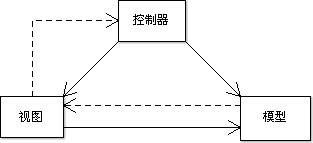
\includegraphics[scale=0.4]{ModelViewControllerDiagram.png}
\caption{MVC设计模式}
\end{figure}

在最初的JSP网页中,数据库查询语句等数据层代码是和HTML表示层代码混杂在一起的,虽然可以将数据从表示层分离开来,但是这样的良好设计通常并不是很容易做到的。

MVC可以从根本上强制性地将数据层和表示层代码分开,尽管构造MVC应用程序需要一些额外的工作,但是MVC带来的好处是毋庸置疑的。

MVC模式的目的是实现一种动态的程序设计,使后续对程序的修改和扩展简化,并且使程序某一部分的重复利用成为可能。

首先,多个 View 能共享一个 Model,这样同一个Web应用程序会提供多种用户界面。例如,用户希望既能够通过浏览器来收发电子邮件,还希望通过手机来访问电子邮箱,因此要求Web网站同时能提供Internet界面和WAP界面。

在MVC设计模式中, Model 响应用户请求并返回响应数据,View 负责格式化数据并把它们呈现给用户,业务逻辑和表示层分离,同一个 Model 可以被不同的 View 重用的做法提高了代码的可重用性。

其次,Controller 是自包含(self-contained)的高独立内聚的对象,与 Model 和 View 保持相对独立,所以可以方便的改变应用程序的数据层和业务规则。例如,把数据库从MySQL移植到Oracle,或者把RDBMS数据源改变成LDAP数据源,只需改变 Model 即可。

Controller 提高了应用程序的灵活性和可配置性。例如,Controller 可以用来连接不同的 Model 和 View 去完成用户的需求,也可以为构造应用程序提供强有力的手段,开发者给定一些可重用的 Model 、 View 和Controller就可以根据用户的需求选择适当的 Model 进行处理,然后选择适当的的 View 将处理结果显示给用户。

在正确地实现了控制器之后,不管数据来自数据库还是LDAP服务器,View 都会正确地显示它们。

除此之外,MVC模式通过对复杂度的简化,使程序结构更加直观,而且软件系统通过对自身基本部分分离的同时也赋予了各个基本部分应有的功能。例如,开发者可以通过自身的专长分组:

\begin{compactitem}
\item 控制器(Controller)- 负责对请求进行处理并转发请求。
\item 视图(View) - 图形界面设计。
\item 模型(Model) - 算法实现、数据管理和数据库设计等具体的功能。
\end{compactitem}

MVC将应用程序划分为三种组件后,开发者就可以设计并定义它们之间的相互作用,因此MVC模式的三个模块是相互独立的,改变其中一个不会影响其他两个,所以依据这种设计思想能构造出良好的少互扰性的构件。

在概念上,MVC模式强调 Model, View, Controller 的分离,各个模块也遵循着由 Controller 来处理消息,Model 掌管数据源,View 负责数据显示的职责分离原则,因此MVC 模式的 Framework在实现上通常会将 MVC 三个部分分离实现:

\begin{compactitem}
\item Model 负责数据访问,现代的 Framework 都会建议使用独立的数据对象 (DTO, POCO, POJO 等) 来替代弱类型的集合对象。

数据访问的代码会使用 Data Access Object或是 ORM-based Framework,也可以进一步使用 Repository Pattern 与 Unit of Works Pattern 来切割数据源的依赖性。

\item Controller 负责处理消息,较高级的 Framework 会有一个默认的实现(例如Spring 的 DispatcherServlet 或是 ASP.NET MVC 的 Controller 等)来作为 Controller 的基础。

在职责分离原则的基础上,每个 Controller 负责的部分不同,因此会将各个 Controller 切割成不同的文件以利于维护。

\item View 负责显示数据,这个部分多为前端应用,而 Controller 会有一个机制将处理的结果 (可能是 Model、集合或状态等) 交给 View,然后由 View 来决定怎么显示。例如 Spring Framework 使用 JSP 或相应技术,ASP.NET MVC 则使用 Razor 处理数据的显示。


\end{compactitem}


MVC 模式强调职责分离会产生很多文件,需要IDE基于类别对象的信息来组织代码编辑,而且 MVC 模式会要求开发者进一步思考应用程序的架构,而非用大杂烩的方式开发应用程序,对于应用程序的生命周期以及后续的可扩充与可维护性而言有相当正面的帮助。

MVC 职责分离也带来了一个现代软件工程要求的重要特性—可测试性 (Testability),基于MVC的应用程序在良好的职责分离的设计下,各个部分都可以独立进行单元测试,因此有利于与企业内的自动化测试、持续集成与持续发布流程的集成,减少应用程序改版部署所需的时间。

MVC 模式的应用程序的目的就是希望打破以往应用程序使用的大杂烩程序开发方式,并间接促使开发人员以更高的架构导向思维来思考应用程序的设计,因此MVC(或是其他的设计模式)都是有助于应用程序长远的发展,大杂烩式的程序在可扩充性和可维护性 (尤其是可测试性) 上远比 MVC 复杂很多。

MVC 模式的应用程序是在初始开发时期必须先思考并使用软件架构,结果就是可扩充性、可维护性和可测试性会因为 MVC 的特性而变得容易。

下面的示例使用JavaScript实现了一个基础的完整MVC示例。

\begin{lstlisting}[language=JavaScript]
/** 模拟Model,View和Controller **/
var M = {}, V = {}, C = {};

/** Model负责存储数据 **/
M.data = "Hello world.";

/** View负责把数据输出到网页上 **/
V.ender = (M) => {alert(M.data)};

/** Controller是Model和View的桥梁 **/
C.handleOnload = () => { V.render(M); }

/** 在网页读取时调用Controller **/
window.onload = C.handleOnload;
\end{lstlisting}

MFC Document/View架构是早期对于MVC模式的实现,MFC将程序分成CView以及CDocument两大类别,其中的Document对应MVC中的 Model ,View 相当于MVC中的 View+Controller,再加上CWinApp类别,合成三大项。


Java EE除了直接以Servlet来编写Controller之外,也可以使用Struts2或Spring Framework等,Model 则是由一个实体Bean来实现,视图(View)可能由JSP来实现。

Java Swing是一个标准的MVC架构,其中ComponentUI代表 View,负责渲染组件,Model 层包括JTextField的Document、JTable的TableModel和JTree的TreeModel等,Event机制可以看作是Controller。

Ruby on Rails的Model 部分使用 Active Record 概念实现,并使用Migration机制来控制Model的结构。

JavaScript的Backbone.js、Angular.js和Ember.js都实现了MVC模式。

PHP的Yaf、CakePHP、CodeIgniter、Symfony、Yii、Phalcon、Laravel和Zend Framework都是MVC框架。


\section{Controller}

控制器(Controller)可以在不同层面间发挥组织作用,从而控制应用程序的流程。

Controller处理事件并作出响应,这里的“事件”包括用户的行为和数据 Model 上的改变等。



Yaf默认的控制器为controllers/Index.php,其内容如下:

\begin{lstlisting}[language=PHP]
<?php
class IndexController extends Yaf_Controller_Abstract {
    /* default action name */
    public function indexAction() {
        $this->_view->word = "hello world, yaf";
        // or
        // $this->getView()->content = "hello world, yaf";
    }
}
\end{lstlisting}

\section{Model}

模型(Model) 用于封装与应用程序的业务逻辑相关的数据以及对数据的处理方法。

“Model”有对数据直接访问的权力(例如对数据库的访问),而且“Model”不依赖“View”和“Controller”。

也就是说, Model 不关心它会被如何显示或是如何被操作,但是 Model 中数据的变化一般会通过一种刷新机制被公布。为了实现这种机制,那些用于监视此 Model 的 View 必须事先在此 Model 上注册,从而View就可以了解在数据 Model 上发生的改变。




\section{View}

虽然理论上并不是必需的,但是视图(View)能够实现数据有目的的显示。

在 View 中一般不包含程序上的逻辑,因此为了实现 View 上的数据刷新功能,View 需要访问它监视的数据模型(Model),应该事先在被它监视的数据那里注册。




Yaf默认的视图文件为application/views/index/index.phtml,Yaf提供了一个默认的模板引擎——Yaf\_View\_Simple来支持使用PHP编码的视图模板。

\begin{lstlisting}[language=HTML]
<html>
  <head>
    <title>Hello world</title>
  </head>
  <body>
     <?php echo $content; ?>
  </body>
</html>
\end{lstlisting}

运行上述的Yaf示例应用程序的输出类似于:


\begin{lstlisting}[language=bash]
<html>
  <head>
    <title>Hello world</title>
  </head>
  <body>
     hello world, yaf
  </body>
</html>
\end{lstlisting}


\chapter{Yaf\_Application}

Yaf\_Application为应用提供了一个辅助设施。

Yaf\_Application提供了可重用的资源、常见的和模块化的引导类以及依赖检查。

和Yii框架的CApplication类一样,Yaf的Yaf\_Application类也实现了单例模式,而且Yaf\_Application不能被序列化和反序列化, 否则当尝试使用PHPUnit来为Yaf写一些测试用例的时候会造成一些不必要的麻烦。

开发者可以使用PHPUnit的@backupGlobals注释来控制全局变量的备份和恢复操作, 从而可以解决上述这个问题。




\begin{lstlisting}[language=PHP]
final Yaf_Application {
  /* 属性 */
  protected $config ;
  protected $dispatcher ;
  protected static $_app ;
  protected $_modules ;
  protected $_running ;
  protected $_environ ;
  /* 方法 */
  public static void app ( void )
  public void bootstrap ([ Yaf_Bootstrap_Abstract $bootstrap ] )
  public Yaf_Application clearLastError ( void )
  private void __clone ( void )
  public __construct ( mixed $config [, string $envrion ] )
  public void __destruct ( void )
  public void environ ( void )
  public void execute ( callable $entry , string $... )
  public Yaf_Application getAppDirectory ( void )
  public Yaf_Config_Abstract getConfig ( void )
  public Yaf_Dispatcher getDispatcher ( void )
  public string getLastErrorMsg ( void )
  public int getLastErrorNo ( void )
  public array getModules ( void )
  public void run ( void )
  public Yaf_Application setAppDirectory ( string $directory )
  private void __sleep ( void )
  private void __wakeup ( void )
}
\end{lstlisting}

\section{Property}


\subsection{\$config}
\subsection{\$dispatcher}
\subsection{\$\_app}
\subsection{\$\_modules}
\subsection{\$\_running}
\subsection{\$\_environ}

\section{Method}


\subsection{Yaf\_Application::app()}

Yaf\_Application::app()方法没有参数。

\begin{lstlisting}[language=PHP]
public static void Yaf_Application::app ( void )
\end{lstlisting}

返回值为当前的Yaf\_Application实例(一个单例模式的对象), 如果在调用之前没有初始化一个Yaf\_Application实例的话,它将返回NULL。

也可以使用Yaf\_Dispatcher::getApplication()来得到Yaf\_Application的实例。











\subsection{Yaf\_Application::bootstrap()}

调用bootstrap(),可以传入一个Yaf\_Bootstrap\_Abstract对象作为可选参数,并返回一个Yaf\_Application实例化对象。

\begin{lstlisting}[language=PHP]
public void Yaf_Application::bootstrap ([ Yaf_Bootstrap_Abstract $bootstrap ] )
\end{lstlisting}

具体来说,Yaf\_Application::bootstrap()方法会指示Yaf\_Application去寻找Bootstrap,并按照声明的顺序,执行所有在Bootstrap类中定义的以\_init开头的方法。 如果没有提供变量bootstrap,Yaf默认会去application.directory中寻找Bootstrap。

\begin{lstlisting}[language=PHP]
<?php
/**
 * This file should be under the APPLICATION_PATH . "/application/"
 * (which was defined in the config passed to Yaf_Application).
 * and named Bootstrap.php,  so the Yaf_Application can find it 
 */
class Bootstrap extends Yaf_Bootstrap_Abstract {
   function _initConfig(Yaf_Dispatcher $dispatcher) {
      echo "1st called\n";
   }
   function _initPlugin($dispatcher) {
      echo "2nd called\n";
   }
}
\end{lstlisting}

\begin{example}
Yaf\_Application::bootstrap()示例
\begin{lstlisting}[language=PHP]
defined('APPLICATION_PATH')  // APPLICATION_PATH will be used in the ini config file
   || define('APPLICATION_PATH', __DIR__); // __DIR__
$application = new Yaf_Application(APPLICATION_PATH.'/conf/application.ini');
$application->bootstrap();
// 以上例程的输出类似于:
1st called
2nd called
\end{lstlisting}
\end{example}


\begin{example}
Yaf\_Application::bootstrap()载入Session类和Database类
\begin{lstlisting}[language=PHP]
<?php
class Bootstrap extends Yaf_Bootstrap_Abstract 
{
   public function _initSession(Yaf_Dispatcher $dispatcher) {
       $session = new Vender\Session();
       $session->start();
   }
   public function _initDatabase(Yaf_Dispatcher $dispatcher) {
       $config = Yaf_Application::app()->getConfig()->application->database;
       Yaf_Registry::set('db', Vendor\Database($config));
   }
}
\end{lstlisting}
\end{example}

\subsection{Yaf\_Application::clearLastError()}

clearLastError()方法没有参数。

\begin{lstlisting}[language=PHP]
public Yaf_Application Yaf_Application::clearLastError ( void )
\end{lstlisting}

清除最后的错误信息,开发者可以自定义错误处理器。


\begin{lstlisting}[language=PHP]
<?php
function error_handler($errno,$errstr,$errfile,$errline) {
   Yaf_Application::app()->clearLastError();
   var_dump(Yaf_Application::app()->getLastErrorNo());
}
$config = array(
   "application"=>array(
      "directory"=>"/tmp/notexists",
      "dispatcher"=>array(
          // trigger error instead of throw exception when error occure
          "throwException"=>0,
      ),
   ),
);
$app = new Yaf_Application($config);
$app->getDispatcher()->setErrorHandler("error_handler",E_RECOVERABLE_ERROR);
$app->run();
// 以上例程的输出类似于:
// int(0)
\end{lstlisting}





\subsection{Yaf\_Application::\_\_clone()}

Yaf\_Application类不允许被克隆,而且\_\_clone()函数没有参数。






\begin{lstlisting}[language=PHP]
private void Yaf_Application::__clone ( void )
\end{lstlisting}





\subsection{Yaf\_Application::\_\_construct()}

构造函数可以初始化一个 Yaf\_Application。




\begin{lstlisting}[language=PHP]
publicYaf_Application::__construct ( mixed $config [, string $envrion ] )
\end{lstlisting}

\begin{compactitem}
\item \$config包含关联数组的配置, 或者一个指向ini格式的配置文件的路径的字符串。
\item \$environ则指示应该载入product还是dev段的配置信息。
\end{compactitem}




如果是一个ini配置文件,那么配置文件中应该有一个定义了yaf.environ 的配置节,这个在生产环境中是默认的。

如果使用了ini配置文件作为应用配置的容器,需要打开yaf.cache\_config 来提升性能。

\begin{lstlisting}[language=PHP]
[product]
;this one should alway be defined, and have no default value
application.directory=APPLICATION_PATH

;following configs have default value, you may no need to define them
application.library = APPLICATION_PATH . "/library"
application.dispatcher.throwException=1
application.dispatcher.catchException=1

application.baseUri=""

;the php script ext name
ap.ext=php

;the view template ext name
ap.view.ext=phtml

ap.dispatcher.defaultModuel=Index
ap.dispatcher.defaultController=Index
ap.dispatcher.defaultAction=index

;defined modules
ap.modules=Index
\end{lstlisting}


\begin{lstlisting}[language=PHP]
<?php
defined('APPLICATION_PATH')                  // APPLICATION_PATH will be used in the ini config file
    || define('APPLICATION_PATH', __DIR__)); //__DIR__ 

$application = new Yaf_Application(APPLICATION_PATH.'/conf/application.ini');
$application->bootstrap()->run();
\end{lstlisting}

向Yaf\_Application传入的配置也可以是一个数组,例如:

\begin{lstlisting}[language=PHP]
<?php
$config = array(
    "application" => array(
        "directory" => realpath(dirname(__FILE__)) . "/application",
    ),
);

/** Yaf_Application */
$application = new Yaf_Application($config);
$application->bootstrap()->run();
\end{lstlisting}



\begin{lstlisting}[language=PHP]

\end{lstlisting}


\subsection{Yaf\_Application::\_\_destruct()}

析构函数(没有参数)






\begin{lstlisting}[language=PHP]
public void Yaf_Application::__destruct ( void )
\end{lstlisting}



\begin{lstlisting}[language=PHP]

\end{lstlisting}



\begin{lstlisting}[language=PHP]

\end{lstlisting}


\subsection{Yaf\_Application::environ()}

获取当前Yaf\_Application的环境名(例如product或dev),它被定义在yaf.environ,默认为product。






\begin{lstlisting}[language=PHP]
public void Yaf_Application::environ ( void )
\end{lstlisting}

environ()方法没有参数。

\begin{lstlisting}[language=PHP]
<?php
$config = array(
    "application" => array(
        "directory" => realpath(dirname(__FILE__)) . "/application",
    ),
);

/** Yaf_Application */
$application = new Yaf_Application($config);
print_r($application->environ());
// 以上例程的输出类似于:
// product
\end{lstlisting}



\begin{lstlisting}[language=PHP]

\end{lstlisting}


\subsection{Yaf\_Application::execute()}

运行回调函数






\begin{lstlisting}[language=PHP]
public void Yaf_Application::execute ( callable $entry , string $... )
\end{lstlisting}

execute()方法通常用于在cron任务中运行Yaf\_Application,而且在cron任务中也可以使用autoloader和Bootstrap机制。

\begin{compactitem}
\item \$entry是一个有效的回调函数
\item \texttt{\$...}是零个或多个要传递给函数的参数
\end{compactitem}



\begin{lstlisting}[language=PHP]
<?php
function main($argc,$argv) {

}
$config = array(
    "application" => array(
        "directory" => realpath(dirname(__FILE__)) . "/application",
    ),
);
/* Yaf_Application */
$application = new Yaf_Application($config);
$application->execute("main", $argc,  $argv);
\end{lstlisting}



\begin{lstlisting}[language=PHP]

\end{lstlisting}


\subsection{Yaf\_Application::getAppDirectory()}

获取Yaf应用程序所在的目录






\begin{lstlisting}[language=PHP]
public Yaf_Application Yaf_Application::getAppDirectory ( void )
\end{lstlisting}



\begin{lstlisting}[language=PHP]

\end{lstlisting}



\begin{lstlisting}[language=PHP]

\end{lstlisting}


\subsection{Yaf\_Application::getConfig()}

获取Yaf\_Config\_Abstract的实例。






\begin{lstlisting}[language=PHP]
public Yaf_Config_Abstract Yaf_Application::getConfig ( void )
\end{lstlisting}

getConfig()方法没有参数,返回值是一个Yaf\_Config\_Abstract类的实例。

\begin{lstlisting}[language=PHP]
<?php
$config = array(
    "application" => array(
        "directory" => realpath(dirname(__FILE__)) . "/application",
    ),
);

/** Yaf_Application */
$application = new Yaf_Application($config);
print_r($application->getConfig());
// 以上例程的输出类似于:
// Yaf_Config_Simple Object
// (
//    [_config:protected] => Array
//        (
//            [application] => Array
//                (
//                    [directory] => /home/laruence/local/www/htdocs/application
//                )
//
//        )
//
//    [_readonly:protected] => 1
// )
\end{lstlisting}






\subsection{Yaf\_Application::getDispatcher()}

获取Yaf\_Dispatcher的实例。



\begin{lstlisting}[language=PHP]
public Yaf_Dispatcher Yaf_Application::getDispatcher ( void )
\end{lstlisting}


\begin{lstlisting}[language=PHP]
<?php
$config = array(
    "application" => array(
        "directory" => realpath(dirname(__FILE__)) . "/application",
    ),
);

/** Yaf_Application */
$application = new Yaf_Application($config);
print_r($application->getDispatcher());
// 以上例程的输出类似于:
// Yaf_Dispatcher Object
// (
//     [_router:protected] => Yaf_Router Object
//         (
//             [_routes:protected] => Array
//                 (
//                     [_default] => Yaf_Route_Static Object
//                         (
//                         )
//                 )
//             [_current:protected] => 
//         )
//     [_view:protected] => 
//     [_request:protected] => Yaf_Request_Http Object
//         (
//             [module] => 
//             [controller] => 
//             [action] => 
//             [method] => Cli
//             [params:protected] => Array
//                 (
//                 )
//             [language:protected] => 
//             [_exception:protected] => 
//             [_base_uri:protected] => 
//             [uri:protected] => 
//             [dispatched:protected] => 
//             [routed:protected] => 
//         )
//     [_plugins:protected] => Array
//         (
//         )
//     [_auto_render:protected] => 1
//     [_return_response:protected] => 
//     [_instantly_flush:protected] => 
//     [_default_module:protected] => Index
//     [_default_controller:protected] => Index
//     [_default_action:protected] => index
//     [_response] => Yaf_Response_Cli Object
//         (
//             [_header:protected] => Array
//                 (
//                 )
//             [_body:protected] => 
//             [_sendheader:protected] => 
//         )
// )
\end{lstlisting}



\subsection{Yaf\_Application::getLastErrorMsg()}

获取最近产生的错误的错误信息。






\begin{lstlisting}[language=PHP]
public string Yaf_Application::getLastErrorMsg ( void )
\end{lstlisting}

\begin{example}
getLstErrorMsg()示例
\begin{lstlisting}[language=PHP]
<?php
function error_handler($errno, $errstr, $errfile, $errline) {
   var_dump(Yaf_Application::app()->getLastErrorMsg());
}

$config = array(                   
 "application" => array(
   "directory" => "/tmp/notexists",
     "dispatcher" => array(
       "throwException" => 0, //trigger error instead of throw exception when error occure
      ),
  ),
);

$app = new Yaf_Application($config);
$app->getDispatcher()->setErrorHandler("error_handler", E_RECOVERABLE_ERROR);
$app->run();
// 以上例程的输出类似于:
// string(69) "Could not find controller script /tmp/notexists/controllers/Index.php"
\end{lstlisting}
\end{example}


\begin{lstlisting}[language=PHP]

\end{lstlisting}


\subsection{Yaf\_Application::getLastErrorNo()}

获取最近产生的错误的错误代码。






\begin{lstlisting}[language=PHP]
public int Yaf_Application::getLastErrorNo ( void )
\end{lstlisting}


\begin{example}
getLstErrorNo()示例
\begin{lstlisting}[language=PHP]
<?php
function error_handler($errno, $errstr, $errfile, $errline) {
   var_dump(Yaf_Application::app()->getLastErrorNo());
   var_dump(Yaf_Application::app()->getLastErrorNo() == YAF_ERR_NOTFOUND_CONTROLLER);
}

$config = array(
  "application" => array(
   "directory" => "/tmp/notexists",
     "dispatcher" => array(
       "throwException" => 0, //trigger error instead of throw exception when error occure
      ),
  ),
);

$app = new Yaf_Application($config);
$app->getDispatcher()->setErrorHandler("error_handler", E_RECOVERABLE_ERROR);
$app->run();
// 以上例程的输出类似于:
// int(516)
// bool(true)
\end{lstlisting}
\end{example}





\subsection{Yaf\_Application::getModules()}

获取在配置文件中声明的模块,如果没有声明,它的默认值将是``Index"。





\begin{lstlisting}[language=PHP]
public array Yaf_Application::getModules ( void )
\end{lstlisting}

\begin{lstlisting}[language=PHP]
<?php
$config = array(
    "application" => array(
        "directory" => realpath(dirname(__FILE__)) . "/application",
    ),
);

/** Yaf_Application */
$application = new Yaf_Application($config);
print_r($application->getModules());
// 以上例程的输出类似于:
// Array
// (
//     [0] => Index
// )
\end{lstlisting}


\subsection{Yaf\_Application::run()}

运行Yaf\_Application(),run()方法本身没有参数。





\begin{lstlisting}[language=PHP]
public void Yaf_Application::run ( void )
\end{lstlisting}

具体来说,run()方法运行一个Yaf\_Application,开始接受并处理请求、分发路由并做出相应的响应,最终将响应返回给客户端。




\subsection{Yaf\_Application::setAppDirectory()}

改变Yaf应用程序的目录到指定的目录。






\begin{lstlisting}[language=PHP]
public Yaf_Application Yaf_Application::setAppDirectory ( string $directory )
\end{lstlisting}



\begin{lstlisting}[language=PHP]

\end{lstlisting}



\begin{lstlisting}[language=PHP]

\end{lstlisting}


\subsection{Yaf\_Application::\_\_sleep()}

Yaf\_Application不能被序列化。






\begin{lstlisting}[language=PHP]
private void Yaf_Application::__sleep ( void )
\end{lstlisting}



\subsection{Yaf\_Application::\_\_wakeup()}

Yaf\_Application不能被反序列化。







\begin{lstlisting}[language=PHP]
private void Yaf_Application::__wakeup ( void )
\end{lstlisting}

\chapter{Yaf\_Bootstrap\_Abstract}

Bootstrap是用来在Application运行(run)之前做一些初始化工作的机制,开发者可以通过继承Yaf\_Bootstrap\_Abstract 来定义自己的Bootstrap类。

在Bootstrap类中所有以``\_init"开头的公有的方法,都会被按照定义顺序依次在Yaf\_Application::bootstrap()方法被调用的时刻进行调用和执行。



\begin{lstlisting}[language=PHP]
<?php
class Bootstrap extends Yaf_Bootstrap_Abstract {
   public function _initConfig(Yaf_Dispatcher $dispatcher) {
       var_dump(__METHOD__);
   }
   public function _initPlugin(Yaf_Dispatcher $dispatcher) {
       var_dump(__METHOD__);
   }
}
$config = array(
   "application"=>array(
       "directory"=>dirname(__FILE__)."/application";
   ),
);
$app=new Yaf_Application($config);
$app->bootstrap();

// 以上例程的输出类似于:
// string(22) "Bootstrap::_initConfig"
// string(22) "Bootstrap::_initPlugin"
\end{lstlisting}





\chapter{Yaf\_Dispatcher}

Yaf\_Dispatcher用于初始化处理请求的运行环境。

具体来说,Yaf\_Dispatcher类协调路由来的请求,并分发和执行发现的动作,然后收集动作产生的响应,输出响应给请求者,并在整个过程完成以后返回响应。

Yaf\_Dispatcher是单例模式运行的,也就是说自始至终只生成一个Yaf\_Dispatcher实例,因此可以把它看成是在分发过程中生成的对象的注册表,可以从中获取到分发过程中产生的对象。



\begin{lstlisting}[language=PHP]
final Yaf_Dispatcher {
  /* 属性 */
  protected $_router ;
  protected $_view ;
  protected $_request ;
  protected $_plugins ;
  protected static $_instance ;
  protected $_auto_render ;
  protected $_return_response ;
  protected $_instantly_flush ;
  protected $_default_module ;
  protected $_default_controller ;
  protected $_default_action ;
  /* 方法 */
  public Yaf_Dispatcher autoRender ( bool $flag )
  public Yaf_Dispatcher catchException ([ bool $flag ] )
  private void __clone ( void )
  public__construct ( void )
  public bool disableView ( void )
  public Yaf_Response_Abstract dispatch ( Yaf_Request_Abstract $request )
  public Yaf_Dispatcher enableView ( void )
  public Yaf_Dispatcher flushInstantly ( bool $flag )
  public Yaf_Application getApplication ( void )
  public static Yaf_Dispatcher getInstance ( void )
  public Yaf_Request_Abstract getRequest ( void )
  public Yaf_Router getRouter ( void )
  public Yaf_View_Interface initView ( string $templates_dir [, array $options ] )
  public Yaf_Dispatcher registerPlugin ( Yaf_Plugin_Abstract $plugin )
  public Yaf_Dispatcher returnResponse ( bool $flag )
  public Yaf_Dispatcher setDefaultAction ( string $action )
  public Yaf_Dispatcher setDefaultController ( string $controller )
  public Yaf_Dispatcher setDefaultModule ( string $module )
  public Yaf_Dispatcher setErrorHandler ( call $callback , int $error_types )
  public Yaf_Dispatcher setRequest ( Yaf_Request_Abstract $request )
  public Yaf_Dispatcher setView ( Yaf_View_Interface $view )
  private void __sleep ( void )
  public Yaf_Dispatcher throwException ([ bool $flag ] )
  private void __wakeup ( void )
}
\end{lstlisting}



\section{Property}





\subsection{\$\_router}

\subsection{\$\_view}
\subsection{\$\_request}
\subsection{\$\_plugins}
\subsection{\$\_instance}
\subsection{\$\_auto\_render}
\subsection{\$\_return\_response}
\subsection{\$\_instantly\_flush}
\subsection{\$\_default\_module}
\subsection{\$\_default\_controller}
\subsection{\$\_default\_action}





\begin{lstlisting}[language=PHP]

\end{lstlisting}



\begin{lstlisting}[language=PHP]

\end{lstlisting}





\begin{lstlisting}[language=PHP]

\end{lstlisting}




\begin{lstlisting}[language=PHP]

\end{lstlisting}



\begin{lstlisting}[language=PHP]

\end{lstlisting}




\begin{lstlisting}[language=PHP]

\end{lstlisting}





\begin{lstlisting}[language=PHP]

\end{lstlisting}




\begin{lstlisting}[language=PHP]

\end{lstlisting}



\begin{lstlisting}[language=PHP]

\end{lstlisting}



\begin{lstlisting}[language=PHP]

\end{lstlisting}














\begin{lstlisting}[language=PHP]

\end{lstlisting}



\begin{lstlisting}[language=PHP]

\end{lstlisting}



\begin{lstlisting}[language=PHP]

\end{lstlisting}

\section{Method}


\subsection{Yaf\_Dispatcher::autoRender()}

开启/关闭自动渲染功能(接受bool型参数)

\begin{lstlisting}[language=PHP]
public Yaf_Dispatcher Yaf_Dispatcher::autoRender ( bool $flag )
\end{lstlisting}

Yaf默认开启自动渲染功能,在开启的情况下,action执行完成以后,Yaf\_Dispatcher 会自动调用view引擎去渲染该action对应的视图模板。 

开发者也可以通过调用这个函数并将 flag 参数的值设为TRUE来进行人工干预。例如,可以在一个action中仅返回FALSE来阻止当前action对应视图的自动渲染。


\begin{lstlisting}[language=PHP]
<?php
class IndexController extends Yaf_Controller_Abstract {
    /* init method will be called as soon as a controller is initialized */ 
    public function init() {
         if($this->getRequest()->isXMLHttpResquest()) {
             //do not call render for ajax request
             //we will outpu a json string
             Yaf_Dispatcher::getInstance()->autoRender(FLASE);
         }
    }
}
\end{lstlisting}



\begin{lstlisting}[language=PHP]

\end{lstlisting}

\subsection{Yaf\_Dispatcher::catchException()}

开启/关闭自动异常捕获功能(接受bool型参数)


\begin{lstlisting}[language=PHP]
public Yaf_Dispatcher Yaf_Dispatcher::catchException ([ bool $flag ] )
\end{lstlisting}

当 application.dispatcher.throwException 开启的时候(也可以通过调用 Yaf\_Dispatcher::throwException(TRUE)() 来开启它),Yaf将会抛出异常而不是触发异常发生。

如果开启了 Yaf\_Dispatcher::catchException() (可以通过设置application.dispatcher.catchException来开启),并且在定义了异常处理的controller的情况下,Yaf会将所有未捕获的异常交给Error Controller的Error Action来处理。例如,捕获异常后可以根据异常代码来渲染指定的异常页面并显示给用户。

\begin{lstlisting}[language=PHP]
<?php
class ErrorController extends Yaf_Controller_Abstract {
    public function init() {}
    /** 
      * you can also call to Yaf_Request_Abstract::getException to  
      * get the un-caught exception.
      */
    public function error($exception) {
        // error occurs
        switch ($exception->getCode()) {
            case YAF_ERR_NOTFOUND_MODULE:
            case YAF_ERR_NOTFOUND_CONTROLLER:
            case YAF_ERR_NOTFOUND_ACTION:
            case YAF_ERR_NOTFOUND_VIEW:
                echo 404, ":",$exception->getMessage();
                break;
            default:
                $message=$exception->getMessage();
                echo 0,":",$exception->getMessage();
                break;
        }
    }
}
// 以上例程的输出类似于:
/* now if some error occur, assuming access a non-exists controller
 * (or you can throw a exception yourself): 
 */
404:Could not find controller script **/application/controllers/No-exists-controller.php
\end{lstlisting}



\subsection{Yaf\_Dispatcher::\_\_clone()}

 Yaf\_Dispatcher 不能被克隆


\begin{lstlisting}[language=PHP]
private void Yaf_Dispatcher::__clone ( void )
\end{lstlisting}




\subsection{Yaf\_Dispatcher::\_\_construct()}

Yaf\_Dispatcher 构造函数

\begin{lstlisting}[language=PHP]
publicYaf_Dispatcher::__construct ( void )
\end{lstlisting}



\subsection{Yaf\_Dispatcher::disableView()}

关闭自动渲染


\begin{lstlisting}[language=PHP]
public bool Yaf_Dispatcher::disableView ( void )
\end{lstlisting}

在一些用户自己会输出信息的情况下使用关闭自动渲染。例如,可以在一个action中仅仅返回FALSE来阻止当前action对应视图的自动渲染。


\subsection{Yaf\_Dispatcher::dispatch()}

分发请求


\begin{lstlisting}[language=PHP]
public Yaf_Response_Abstract Yaf_Dispatcher::dispatch ( Yaf_Request_Abstract $request )
\end{lstlisting}

Yaf\_Dispatcher 的dispatch()方法的工作非常繁重,而且它还需要一个request对象。

分发请求的过程有三个不同的事件:

\begin{compactitem}
\item 路由
\item 分发
\item 响应
\end{compactitem}

路由只发生一次,当dispatch()被调用的时候,需要使用请求对象中的值(例如PATH\_INFO)。

分发发生在一个循环中,一个请求可能会分发出多个action, 或者controller或者一个plugin可能重置请求对象来强制分发其他的action。 

当所有分发的步骤都执行完毕,Yaf\_Dispatcher 会返回一个响应,因此如果中途出错,可以执行exit()来直接返回输出,其他未指定的操作就不需要再继续执行。





\subsection{Yaf\_Dispatcher::enableView()}

开启自动渲染


\begin{lstlisting}[language=PHP]
public Yaf_Dispatcher Yaf_Dispatcher::enableView ( void )
\end{lstlisting}

如果前面的步骤禁用了自动渲染,在后面的步骤中还可以通过调用enableView()方法来重新开启自动渲染。

\begin{lstlisting}[language=PHP]

\end{lstlisting}
\subsection{Yaf\_Dispatcher::flushInstantly()}

打开关闭自动响应

\begin{lstlisting}[language=PHP]
public Yaf_Dispatcher Yaf_Dispatcher::flushInstantly ( bool $flag )
\end{lstlisting}


\subsection{Yaf\_Dispatcher::getApplication()}

和Yaf\_Application::app()的执行结果相同,二者都是获取当前的Yaf\_Application实例。


\begin{lstlisting}[language=PHP]
public Yaf_Application Yaf_Dispatcher::getApplication ( void )
\end{lstlisting}






\subsection{Yaf\_Dispatcher::getInstance()}


获取当前的Yaf\_Dispatcher实例

\begin{lstlisting}[language=PHP]
public static Yaf_Dispatcher Yaf_Dispatcher::getInstance ( void )
\end{lstlisting}



\subsection{Yaf\_Dispatcher::getRequest()}


获取当前的请求实例

\begin{lstlisting}[language=PHP]
public Yaf_Request_Abstract Yaf_Dispatcher::getRequest ( void )
\end{lstlisting}





\subsection{Yaf\_Dispatcher::getRouter()}

获取路由器


\begin{lstlisting}[language=PHP]
public Yaf_Router Yaf_Dispatcher::getRouter ( void )
\end{lstlisting}





\subsection{Yaf\_Dispatcher::initView()}

初始化视图引擎并返回它


\begin{lstlisting}[language=PHP]
public Yaf_View_Interface Yaf_Dispatcher::initView ( string $templates_dir [, array $options ] )
\end{lstlisting}

在初始化视图引擎时可以传入视图模板的目录,以及可选参数。



\subsection{Yaf\_Dispatcher::registerPlugin()}


注册一个插件


\begin{lstlisting}[language=PHP]
public Yaf_Dispatcher Yaf_Dispatcher::registerPlugin ( Yaf_Plugin_Abstract $plugin )
\end{lstlisting}


\begin{lstlisting}[language=PHP]
<?php
class Bootstrap extends Yaf_Bootstrap_Abstract {
   public function _initPlugin(Yaf_Dispatcher $dispatcher) {
        /**
         * Yaf assumes plugin scripts under [application.directory] .  "/plugins" 
         * for this case, it will be:
         * [application.directory] . "/plugins/" . "User" . [application.ext]
         */ 
        $user=new UserPlugin();
        $dispatcher->registerPlugin($user);
   }
}
\end{lstlisting}

Yaf假设插件脚本位于plugins目录下。




\subsection{Yaf\_Dispatcher::returnResponse()}

是否返回响应。

\begin{lstlisting}[language=PHP]
public Yaf_Dispatcher Yaf_Dispatcher::returnResponse ( bool $flag )
\end{lstlisting}

\subsection{Yaf\_Dispatcher::setDefaultAction()}

设置路由的默认动作(传入指定的Action名字)

\begin{lstlisting}[language=PHP]
public Yaf_Dispatcher Yaf_Dispatcher::setDefaultAction ( string $action )
\end{lstlisting}


\subsection{Yaf\_Dispatcher::setDefaultController()}

设置路由的默认控制器(传入指定的控制器名字)

\begin{lstlisting}[language=PHP]
public Yaf_Dispatcher Yaf_Dispatcher::setDefaultController ( string $controller )
\end{lstlisting}

\subsection{Yaf\_Dispatcher::setDefaultModule()}

设置路由的默认模块(传入指定的模块名字)

\begin{lstlisting}[language=PHP]
public Yaf_Dispatcher Yaf_Dispatcher::setDefaultModule ( string $module )
\end{lstlisting}

\subsection{Yaf\_Dispatcher::setErrorHandler()}

设置错误处理函数。例如,如果在application.dispatcher.throwException关闭的情况下,Yaf会在出错的时候触发错误,这个时候如果设置了错误处理函数,则会把控制交给错误处理函数处理,因此当错误发生的时候这个错误处理函数将被调用。

\begin{compactitem}
\item \$callback:错误处理的回调函数
\item \$error\_type:错误类型
\end{compactitem}



\begin{lstlisting}[language=PHP]
<?php
$dispatcher->setErrorHandler(array(get_class($this),'error_handler'));
\end{lstlisting}


\subsection{Yaf\_Dispatcher::setRequest()}

设置请求

\begin{lstlisting}[language=PHP]
public Yaf_Dispatcher Yaf_Dispatcher::setRequest ( Yaf_Request_Abstract $request )
\end{lstlisting}


\subsection{Yaf\_Dispatcher::setView()}

设置视图引擎(默认传入Yaf\_View\_Interface的实例)

\begin{lstlisting}[language=PHP]
public Yaf_Dispatcher Yaf_Dispatcher::setView ( Yaf_View_Interface $view )
\end{lstlisting}

Yaf提供了一个试图引擎——Yaf\_View\_Simple,如果需要使用自定义的视图引擎代替 Yaf\_View\_Simple , 这个函数可以解决这个问题。


\begin{example}
使用Smarty代替默认的视图引擎
\begin{lstlisting}[language=PHP]
<?php
require "/path/to/smarty/Smarty.class.php";

class Smarty_Adapter implements Yaf_View_Interface
{
    /**
     * Smarty object
     * @var Smarty
     */
    public $_smarty;
 
    /**
     * Constructor
     *
     * @param string $tmplPath
     * @param array $extraParams
     * @return void
     */
    public function __construct($tmplPath = null, $extraParams = array()) {
        $this->_smarty = new Smarty;
 
        if (null !== $tmplPath) {
            $this->setScriptPath($tmplPath);
        }
 
        foreach ($extraParams as $key => $value) {
            $this->_smarty->$key = $value;
        }
    }
 
    /**
     * Set the path to the templates
     *
     * @param string $path The directory to set as the path.
     * @return void
     */
    public function setScriptPath($path)
    {
        if (is_readable($path)) {
            $this->_smarty->template_dir = $path;
            return;
        }
 
        throw new Exception('Invalid path provided');
    }
 
    /**
     * Assign a variable to the template
     *
     * @param string $key The variable name.
     * @param mixed $val The variable value.
     * @return void
     */
    public function __set($key, $val)
    {
        $this->_smarty->assign($key, $val);
    }
 
    /**
     * Allows testing with empty() and isset() to work
     *
     * @param string $key
     * @return boolean
     */
    public function __isset($key)
    {
        return (null !== $this->_smarty->get_template_vars($key));
    }
 
    /**
     * Allows unset() on object properties to work
     *
     * @param string $key
     * @return void
     */
    public function __unset($key)
    {
        $this->_smarty->clear_assign($key);
    }
 
    /**
     * Assign variables to the template
     *
     * Allows setting a specific key to the specified value, OR passing
     * an array of key => value pairs to set en masse.
     *
     * @see __set()
     * @param string|array $spec The assignment strategy to use (key or
     * array of key => value pairs)
     * @param mixed $value (Optional) If assigning a named variable,
     * use this as the value.
     * @return void
     */
    public function assign($spec, $value = null) {
        if (is_array($spec)) {
            $this->_smarty->assign($spec);
            return;
        }
 
        $this->_smarty->assign($spec, $value);
    }
 
    /**
     * Clear all assigned variables
     *
     * Clears all variables assigned to Yaf_View either via
     * {@link assign()} or property overloading
     * ({@link __get()}/{@link __set()}).
     *
     * @return void
     */
    public function clearVars() {
        $this->_smarty->clear_all_assign();
    }
 
    /**
     * Processes a template and returns the output.
     *
     * @param string $name The template to process.
     * @return string The output.
     */
    public function render($name, $value = NULL) {
        return $this->_smarty->fetch($name);
    }

    public function display($name, $value = NULL) {
        echo $this->_smarty->fetch($name);
    }
}
\end{lstlisting}
\end{example}

\begin{example}
使用Yaf\_Dispatcher::setView()设置视图渲染引擎
\begin{lstlisting}[language=PHP]
<?php
class Bootstrap extends Yaf_Bootstrap_Abstract {
    /**
     * there are some config for smarty in the config:
     *
     * smarty.left_delimiter   = "{{"
     * smarty.right_delimiter  = "}}"
     * smarty.template_dir     = APPLICATION_PATH "/views/scripts/"
     * smarty.compile_dir      = APPLICATION_PATH "/views/templates_c/"
     * smarty.cache_dir        = APPLICATION_PATH "/views/templates_d/"
     *
     */
    public function _initConfig() {
        $config = Yaf_Applicatin::app()->getConfig();
        Yaf_Registry::set('config',$config);
    }
    
    public function _initLocalName() {
        /** we put class Smarty_Adapter under the local library directory */
        Yaf\_Loader::getInstance()->registerLocalNamespace('Smarty');
    }
    
    public function _initSmarty(Yaf_Dispatcher $dispatcher) {
        $smarty = new Smarty_Adapter(null,Yaf_Registry::get('config')->get('smarty');
        $dispatcher->setView($smarty);
         /* now the Smarty view engine become the default view engine of Yaf */
    }
}
\end{lstlisting}
\end{example}

\subsection{Yaf\_Dispatcher::\_\_sleep()}

Yaf\_Dispatcher 不能被序列化

\begin{lstlisting}[language=PHP]
private void Yaf_Dispatcher::__sleep ( void )
\end{lstlisting}

\subsection{Yaf\_Dispatcher::throwException()}

开启/关闭异常抛出

\begin{lstlisting}[language=PHP]
public Yaf_Dispatcher Yaf_Dispatcher::throwException ([ bool $flag ] )
\end{lstlisting}

Yaf\_Dispatcher可以设置当意外的错误发生时是否开启/关闭异常抛出。其中,当开启的时候,Yaf将会抛出异常而不是触发可捕捉的错误。

另外,也可以使用 application.dispatcher.throwException来达到相同的目的。

\begin{example}
Yaf\_Dispatcher开启异常捕获的示例
\begin{lstlisting}[language=PHP]
<?php
$config = array(
    'application' => array(
        'directory' => dirname(__FILE__),
    ),
);
$app = new Yaf_Application($config);

$app->getDispatcher()->throwException(true);

try {
    $app->run();
} catch (Yaf_Exception $e) {
    var_dump($e->getMessage());
}
// 以上例程的输出类似于:
// string(59) "Could not find controller script /tmp/controllers/Index.php"
\end{lstlisting}
\end{example}


\begin{example}
Yaf\_Dispatcher关闭异常捕获的示例
\begin{lstlisting}[language=PHP]
<?php
$config = array(
    'application' => array(
        'directory' => dirname(__FILE__),
    ),
);
$app = new Yaf_Application($config);

$app->getDispatcher()->throwException(false);

$app->run();
?>
// 以上例程的输出类似于:
// PHP Catchable fatal error:  Yaf_Application::run(): 
// Could not find controller script /tmp/controllers/Index.php in /tmp/1.php on line 12
\end{lstlisting}
\end{example}


\subsection{Yaf\_Dispatcher::\_\_wakeup()}

Yaf\_Dispatcher 不能被反序列化

\begin{lstlisting}[language=PHP]
private void Yaf_Dispatcher::__wakeup ( void )
\end{lstlisting}



\chapter{Yaf\_Config\_Abstract}

\begin{lstlisting}[language=PHP]
abstract Yaf_Config_Abstract {
  /* 属性 */
  protected $_config ;
  protected $_readonly ;
  /* 方法 */
  abstract public mixed get ( string $name , mixed $value )
  abstract public bool readonly ( void )
  abstract public Yaf_Config_Abstract set ( void )
  abstract public array toArray ( void )
}
\end{lstlisting}

\section{Property}


\subsection{\$\_config}


\subsection{\$\_readonly}



\section{Method}


\subsection{Yaf\_Config\_Abstract::get()}


getter







\begin{lstlisting}[language=PHP]
abstract public mixed Yaf_Config_Abstract::get ( string $name , mixed $value )
\end{lstlisting}



\subsection{Yaf\_Config\_Abstract::readonly()}


寻找只读配置





\begin{lstlisting}[language=PHP]
bstract public bool Yaf_Config_Abstract::readonly ( void )
\end{lstlisting}

\subsection{Yaf\_Config\_Abstract::set()}

setter


\begin{lstlisting}[language=PHP]
abstract public Yaf_Config_Abstract Yaf_Config_Abstract::set ( void )
\end{lstlisting}

\subsection{Yaf\_Config\_Abstract::toArray()}

转换为数组

\begin{lstlisting}[language=PHP]
abstract public array Yaf_Config_Abstract::toArray ( void )
\end{lstlisting}



\chapter{Yaf\_Config\_Ini}



Yaf\_Config\_Ini允许开发者通过嵌套的对象属性语法在应用程序中用熟悉的INI格式存储和读取配置数据。 INI格式在提供拥有配置数据键的等级结构和配置数据节之间的继承能力方面具有专长。

配置数据等级结构通过用点或者句号(.)分离键值。 一个节可以扩展或者通过在节的名称之后带一个冒号(:)和被继承的配置数据的节的名称来从另一个节继承。

parse\_ini\_file()函数和 php.ini 文件没有关系,该文件在运行脚本时就已经处理过了,parse\_ini\_file()函数可以用来读取你自己的应用程序的配置文件。

如果 ini 文件中的值包含任何非字母数字的字符,需要将其括在双引号中(\texttt{"})。

注意,有些保留字不能作为 ini 文件中的键名,包括null,yes,no,true 和 false,其中:

\begin{compactitem}
\item 值为 null,no 和 false 等效于\texttt{""}
\item 值为 yes 和 true 等效于\texttt{"1"}
\end{compactitem}

字符 \texttt{\{\}|\&\~{}![()"} 也不能用在键名的任何地方,而且这些字符在选项值中有着特殊的意义。

具体来说,Yaf\_Config\_Ini利用PHP的函数parse\_ini\_file()来解析配置文件,Yaf\_Config\_Ini的值可能传递给parse\_ini\_file()函数的值可能包括``TRUE", ``FALSE",``yes", ``no"和``NULL"等。

\begin{lstlisting}[language=PHP]
Yaf_Config_Ini extends Yaf_Config_Abstract implements Iterator , Traversable , ArrayAccess , Countable {
  /* 属性 */
  /* 方法 */
  public __construct ( string $config_file [, string $section ] )
  public void count ( void )
  public void current ( void )
  public void __get ([ string $name ] )
  public void __isset ( string $name )
  public void key ( void )
  public void next ( void )
  public void offsetExists ( string $name )
  public void offsetGet ( string $name )
  public void offsetSet ( string $name , string $value )
  public void offsetUnset ( string $name )
  public void readonly ( void )
  public void rewind ( void )
  public void __set ( string $name , mixed $value )
  public void toArray ( void )
  public void valid ( void )
  /* 继承的方法 */
  abstract public mixed Yaf_Config_Abstract::get ( string $name , mixed $value )
  abstract public bool Yaf_Config_Abstract::readonly ( void )
  abstract public Yaf_Config_Abstract Yaf_Config_Abstract::set ( void )
  abstract public array Yaf_Config_Abstract::toArray ( void )
}
\end{lstlisting}


这个例子说明了使用Yaf\_Config\_Ini从一个INI配置文件中获取配置数据的基本用法。 这个例子中既有生产环境的配置方法也有演示环境的配置方法。 因为演示环境的配置跟生产环境的非常类似,所以演示环境的配置继承了生产环境的配置。 

在复杂的情况下,决定是任意的,也可以写成相反的。在更复杂的情况下,生产环境继承自演示环境不是不可能的。 假设,以下配置数据都包含在/path/to/config.ini中:

\begin{lstlisting}[language=bash]
; Production site configuration data
[production]
webhost                  = www.example.com
database.adapter         = pdo_mysql
database.params.host     = db.example.com
database.params.username = dbuser
database.params.password = secret
database.params.dbname   = dbname
 
; Staging site configuration data inherits from production and
; overrides values as necessary
[staging : production]
database.params.host     = dev.example.com
database.params.username = devuser
database.params.password = devsecret
\end{lstlisting}



\begin{example}
使用Yaf\_Config\_Ini从INI配置文件中获取配置信息
\begin{lstlisting}[language=PHP]
<?php
$config = new Yaf_Config_Ini('/path/to/config.ini','staging');
var_dump($config->database->params->host); 
var_dump($config->database->params->dbname);
var_dump($config->get("database.params.username"));
// 以上例程的输出类似于:
// string(15) "dev.example.com"
// string(6) "dbname"
// string(7) "devuser
\end{lstlisting}
\end{example}


\section{Property}

\subsection{\$\_config}



\subsection{\$\_readonly}


\section{Method}


\subsection{Yaf\_Config\_Ini::\_\_construct()}


构造函数




\begin{lstlisting}[language=PHP]
public Yaf_Config_Ini::__construct ( string $config_file [, string $section ] )
\end{lstlisting}








\subsection{Yaf\_Config\_Ini::count()}

返回配置的节数量


\begin{lstlisting}[language=PHP]
public void Yaf_Config_Ini::count ( void )
\end{lstlisting}



\begin{lstlisting}[language=PHP]

\end{lstlisting}


\subsection{Yaf\_Config\_Ini::current()}


返回当前节点

\begin{lstlisting}[language=PHP]
public void Yaf_Config_Ini::current ( void )
\end{lstlisting}



\begin{lstlisting}[language=PHP]

\end{lstlisting}



\subsection{Yaf\_Config\_Ini::\_\_get()}


读取节点配置

\begin{lstlisting}[language=PHP]
public void Yaf_Config_Ini::__get ([ string $name ] )
\end{lstlisting}



\begin{lstlisting}[language=PHP]

\end{lstlisting}


\subsection{Yaf\_Config\_Ini::\_\_isset()}

检查节点是否存在

\begin{lstlisting}[language=PHP]
public void Yaf_Config_Ini::__isset ( string $name )
\end{lstlisting}


\subsection{Yaf\_Config\_Ini::key()}

返回当前元素的键


\begin{lstlisting}[language=PHP]
public void Yaf_Config_Ini::key ( void )
\end{lstlisting}



\begin{lstlisting}[language=PHP]

\end{lstlisting}


\subsection{Yaf\_Config\_Ini::next()}

向前移动到下一个元素

\begin{lstlisting}[language=PHP]
public void Yaf_Config_Ini::next ( void )
\end{lstlisting}

\begin{lstlisting}[language=PHP]

\end{lstlisting}



\subsection{Yaf\_Config\_Ini::offsetExists()}

检查一个偏移位置是否存在

\begin{lstlisting}[language=PHP]
public void Yaf_Config_Ini::offsetExists ( string $name )
\end{lstlisting}

\begin{lstlisting}[language=PHP]

\end{lstlisting}



\subsection{Yaf\_Config\_Ini::offsetGet()}

获取一个偏移位置的值

\begin{lstlisting}[language=PHP]
public void Yaf_Config_Ini::offsetGet ( string $name )
\end{lstlisting}

\begin{lstlisting}[language=PHP]

\end{lstlisting}


\subsection{Yaf\_Config\_Ini::offsetSet()}

设置一个偏移位置的值

\begin{lstlisting}[language=PHP]
public void Yaf_Config_Ini::offsetSet ( string $name , string $value )
\end{lstlisting}

\begin{lstlisting}[language=PHP]

\end{lstlisting}


\subsection{Yaf\_Config\_Ini::offsetUnset()}

复位一个偏移位置的值

\begin{lstlisting}[language=PHP]
public void Yaf_Config_Ini::offsetUnset ( string $name )
\end{lstlisting}


\subsection{Yaf\_Config\_Ini::readonly()}

检查配置是否只读

\begin{lstlisting}[language=PHP]
public void Yaf_Config_Ini::readonly ( void )
\end{lstlisting}

\begin{lstlisting}[language=PHP]

\end{lstlisting}



\subsection{Yaf\_Config\_Ini::rewind()}

检查当前位置是否有效

\begin{lstlisting}[language=PHP]
public void Yaf_Config_Ini::rewind ( void )
\end{lstlisting}

\begin{lstlisting}[language=PHP]

\end{lstlisting}



\subsection{Yaf\_Config\_Ini::\_\_set()}

设置节点配置

\begin{lstlisting}[language=PHP]
public void Yaf_Config_Ini::__set ( string $name , mixed $value )
\end{lstlisting}

\begin{lstlisting}[language=PHP]

\end{lstlisting}



\subsection{Yaf\_Config\_Ini::toArray()}

转换为数组的格式

\begin{lstlisting}[language=PHP]
public void Yaf_Config_Ini::toArray ( void )
\end{lstlisting}

\begin{lstlisting}[language=PHP]

\end{lstlisting}



\subsection{Yaf\_Config\_Ini::valid()}

检查迭代器是否有效

\begin{lstlisting}[language=PHP]
public void Yaf_Config_Ini::valid ( void )
\end{lstlisting}


\chapter{Yaf\_Config\_Simple}


Yaf\_Config\_Simple 是 Yaf\_Config\_ini 的简洁版本,只允许传入数组进行初始化,并提供了设置readonly的参数。

\begin{lstlisting}[language=PHP]
Yaf_Config_Simple extends Yaf_Config_Abstract implements Iterator , Traversable , ArrayAccess , Countable {
  /* 属性 */
  protected $_readonly ;
  /* 方法 */
  public __construct ( string $config_file [, string $section ] )
  public void count ( void )
  public void current ( void )
  public void __get ([ string $name ] )
  public void __isset ( string $name )
  public void key ( void )
  public void next ( void )
  public void offsetExists ( string $name )
  public void offsetGet ( string $name )
  public void offsetSet ( string $name , string $value )
  public void offsetUnset ( string $name )
  public void readonly ( void )
  public void rewind ( void )
  public void __set ( string $name , string $value )
  public void toArray ( void )
  public void valid ( void )
  /* 继承的方法 */
  abstract public mixed Yaf_Config_Abstract::get ( string $name , mixed $value )
  abstract public bool Yaf_Config_Abstract::readonly ( void )
  abstract public Yaf_Config_Abstract Yaf_Config_Abstract::set ( void )
  abstract public array Yaf_Config_Abstract::toArray ( void )
}
\end{lstlisting}


\section{Property}

\subsection{\$\_config}



\subsection{\$\_readonly}


\section{Method}


\subsection{Yaf\_Config\_Simple::\_\_construct()}


构造函数




\begin{lstlisting}[language=PHP]
public Yaf_Config_Simple::__construct ( string $config_file [, string $section ] )
\end{lstlisting}








\subsection{Yaf\_Config\_Simple::count()}

返回配置的节数量


\begin{lstlisting}[language=PHP]
public void Yaf_Config_Simple::count ( void )
\end{lstlisting}



\begin{lstlisting}[language=PHP]

\end{lstlisting}


\subsection{Yaf\_Config\_Simple::current()}


返回当前节点

\begin{lstlisting}[language=PHP]
public void Yaf_Config_Simple::current ( void )
\end{lstlisting}



\begin{lstlisting}[language=PHP]

\end{lstlisting}



\subsection{Yaf\_Config\_Simple::\_\_get()}


读取节点配置

\begin{lstlisting}[language=PHP]
public void Yaf_Config_Simple::__get ([ string $name ] )
\end{lstlisting}



\begin{lstlisting}[language=PHP]

\end{lstlisting}


\subsection{Yaf\_Config\_Simple::\_\_isset()}

检查节点是否存在

\begin{lstlisting}[language=PHP]
public void Yaf_Config_Simple::__isset ( string $name )
\end{lstlisting}


\subsection{Yaf\_Config\_Simple::key()}

返回当前元素的键


\begin{lstlisting}[language=PHP]
public void Yaf_Config_Simple::key ( void )
\end{lstlisting}



\begin{lstlisting}[language=PHP]

\end{lstlisting}


\subsection{Yaf\_Config\_Simple::next()}

向前移动到下一个元素

\begin{lstlisting}[language=PHP]
public void Yaf_Config_Simple::next ( void )
\end{lstlisting}

\begin{lstlisting}[language=PHP]

\end{lstlisting}



\subsection{Yaf\_Config\_Simple::offsetExists()}

检查一个偏移位置是否存在

\begin{lstlisting}[language=PHP]
public void Yaf_Config_Simple::offsetExists ( string $name )
\end{lstlisting}

\begin{lstlisting}[language=PHP]

\end{lstlisting}



\subsection{Yaf\_Config\_Simple::offsetGet()}

获取一个偏移位置的值

\begin{lstlisting}[language=PHP]
public void Yaf_Config_Simple::offsetGet ( string $name )
\end{lstlisting}

\begin{lstlisting}[language=PHP]

\end{lstlisting}


\subsection{Yaf\_Config\_Simple::offsetSet()}

设置一个偏移位置的值

\begin{lstlisting}[language=PHP]
public void Yaf_Config_Simple::offsetSet ( string $name , string $value )
\end{lstlisting}

\begin{lstlisting}[language=PHP]

\end{lstlisting}


\subsection{Yaf\_Config\_Simple::offsetUnset()}

复位一个偏移位置的值

\begin{lstlisting}[language=PHP]
public void Yaf_Config_Simple::offsetUnset ( string $name )
\end{lstlisting}


\subsection{Yaf\_Config\_Simple::readonly()}

检查配置是否只读

\begin{lstlisting}[language=PHP]
public void Yaf_Config_Simple::readonly ( void )
\end{lstlisting}

\begin{lstlisting}[language=PHP]

\end{lstlisting}



\subsection{Yaf\_Config\_Simple::rewind()}

检查当前位置是否有效

\begin{lstlisting}[language=PHP]
public void Yaf_Config_Simple::rewind ( void )
\end{lstlisting}

\begin{lstlisting}[language=PHP]

\end{lstlisting}



\subsection{Yaf\_Config\_Simple::\_\_set()}

设置节点配置

\begin{lstlisting}[language=PHP]
public void Yaf_Config_Simple::__set ( string $name , string $value )
\end{lstlisting}

\begin{lstlisting}[language=PHP]

\end{lstlisting}



\subsection{Yaf\_Config\_Simple::toArray()}

转换为数组的格式

\begin{lstlisting}[language=PHP]
public void Yaf_Config_Simple::toArray ( void )
\end{lstlisting}

\begin{lstlisting}[language=PHP]

\end{lstlisting}



\subsection{Yaf\_Config\_Simple::valid()}

检查迭代器是否有效

\begin{lstlisting}[language=PHP]
public void Yaf_Config_Simple::valid ( void )
\end{lstlisting}




\chapter{Yaf\_Controller\_Abstract}


Yaf\_Controller\_Abstract是Yaf的MVC体系的核心部分,每个用户自定义controller都应当继承Yaf\_Controller\_Abstract。

在用户自己定义的controller中无法调用\_\_construct方法,Yaf\_Controller\_Abstract 提供了一个魔术方法Yaf\_Controller\_Abstract::init(),这样当controller被实例化的时候,init()将被调用。

Action可能需要参数。例如,当一个请求来到的时候,在路由中如果请求的参数有相同名称的变量(例如Yaf\_Request\_Abstract::getParam()), Yaf将把参数传递给action方法(Yaf\_Action\_Abstract::execute())。





\begin{lstlisting}[language=PHP]
abstract Yaf_Controller_Abstract {
   /* 属性 */
   public $actions ;
   protected $_module ;
   protected $_name ;
   protected $_request ;
   protected $_response ;
   protected $_invoke_args ;
   protected $_view ;
   /* 方法 */
   final private void __clone ( void )
   final private __construct ( void )
   protected bool display ( string $tpl [, array $parameters ] )
   public void forward ( string $module [, string $controller [, string $action [, array $paramters ]]] )
   public void getInvokeArg ( string $name )
   public void getInvokeArgs ( void )
   public string getModuleName ( void )
   public Yaf_Request_Abstract getRequest ( void )
   public Yaf_Response_Abstract getResponse ( void )
   public Yaf_View_Interface getView ( void )
   public void getViewpath ( void )
   public void init ( void )
   public void initView ([ array $options ] )
   public void redirect ( string $url )
   protected string render ( string $tpl [, array $parameters ] )
   public void setViewpath ( string $view_directory )
}
\end{lstlisting}

\section{Property}


\subsection{\$actions}

开发者可以通过使用\$actions和 Yaf\_Action\_Abstract 在一个单独的PHP脚本中定义action函数。



\begin{example}
在独立的脚本中定义action
\begin{lstlisting}[language=PHP]
<?php
class IndexController extends Yaf_Controller_Abstract {
    protected $actions = array(
         /** now dummyAction is defined in a separate file */
         "dummy"=>"actions/Dummy_action.php",
    );
    
    /**/
    public function indexAction($name,$id){
         assert($name == $this->getRequest()->getParam("name"));
         assert($id == $this->_request->getParam("id"));
    }
}
\end{lstlisting}
\end{example}

\begin{example}
Dummy\_action.php
\begin{lstlisting}[language=PHP]
<?php
class DummyAction extends Yaf_Action_Abstract {
    /* a action class shall define this method  as the entry point */
    public function excute() {
    
    }
}
\end{lstlisting}
\end{example}

\subsection{\$\_module}

模块名

\subsection{\$\_name}



\subsection{\$\_request}

当前的请求实例


\subsection{\$\_response}

当前的响应实例


\subsection{\$\_invoke\_args}



\subsection{\$\_view}

视图引擎


\section{Method}


\subsection{Yaf\_Controller\_Abstract::\_\_clone()}


Yaf\_Controller\_Abstract 不能被克隆


\begin{lstlisting}[language=PHP]
final private void Yaf_Controller_Abstract::__clone ( void )
\end{lstlisting}


\subsection{Yaf\_Controller\_Abstract::\_\_construct()}

Yaf\_Controller\_Abstract 构造函数


\begin{lstlisting}[language=PHP]
final private Yaf_Controller_Abstract::__construct ( void )
\end{lstlisting}


\subsection{Yaf\_Controller\_Abstract::display()}


输出页面





\begin{lstlisting}[language=PHP]
protected bool Yaf_Controller_Abstract::display ( string $tpl [, array $parameters ] )
\end{lstlisting}



\begin{lstlisting}[language=PHP]

\end{lstlisting}

\subsection{Yaf\_Controller\_Abstract::forward()}

转发请求(在转发失败时FALSE)

\begin{lstlisting}[language=PHP]
public void Yaf_Controller_Abstract::forward ( string $module [, string $controller [, string $action [, array $paramters ]]] )
\end{lstlisting}

forward()将当前的请求转交给另外的Action,而且调用Yaf\_Controller\_Abstract::forward()以后不会直接立即跳转到目的Action执行,而是会在当前的Action执行完成后,在下一轮的DispatchLoop中才会交给目的Action。

如果希望立即跳转到目的Action,那么需要使用return结束当前的执行流程并立刻跳转。


\begin{compactitem}
\item module

要跳转的目的Action的Module, 如果是NULL, 则默认Module会被采用.

\item controller

要跳转的目的Action的Controller, 如果是NULL, 则默认Controller会被采用.

\item action

要跳转的目的Action.

\item paramters

跳转参数, 可以在目的Action中通过Yaf\_Request\_Abstrace::getParam()来获取.

\end{compactitem}


\begin{lstlisting}[language=PHP]
<?php
class IndexController extends Yaf\_Controller\_Abstract {
    public function indexAction() {
        $logined = $_SESSION['login'];
        if(!$login) {
            $this->forward('login', array('from'=>'Index'));
            return false;
        }
        // other process
    }
    
    public function loginAction() {
        echo 'login, redirected from',$this->_request->getParam('from'), ' action';
    }
}
// 以上例程的输出类似于:
// login, redirected from Index action
\end{lstlisting}

\subsection{Yaf\_Controller\_Abstract::getInvokeArg()}


\begin{lstlisting}[language=PHP]
public void Yaf_Controller_Abstract::getInvokeArg ( string $name )
\end{lstlisting}




\subsection{Yaf\_Controller\_Abstract::getInvokeArgs()}


\begin{lstlisting}[language=PHP]
public void Yaf_Controller_Abstract::getInvokeArgs ( void )
\end{lstlisting}

\subsection{Yaf\_Controller\_Abstract::getModuleName()}

获取当前控制器所属的模块名




\begin{lstlisting}[language=PHP]
public string Yaf_Controller_Abstract::getModuleName ( void )
\end{lstlisting}


\subsection{Yaf\_Controller\_Abstract::getRequest()}

获取请求实例

\begin{lstlisting}[language=PHP]
public Yaf_Request_Abstract Yaf_Controller_Abstract::getRequest ( void )
\end{lstlisting}

\subsection{Yaf\_Controller\_Abstract::getResponse()}

获取响应实例

\begin{lstlisting}[language=PHP]
public Yaf_Response_Abstract Yaf_Controller_Abstract::getResponse ( void )
\end{lstlisting}

\subsection{Yaf\_Controller\_Abstract::getView()}

获取当前的视图引擎

\begin{lstlisting}[language=PHP]
public void Yaf_Controller_Abstract::getViewpath ( void )
\end{lstlisting}

\subsection{Yaf\_Controller\_Abstract::getViewPath()}

获取当前的视图引擎的路径

\begin{lstlisting}[language=PHP]

\end{lstlisting}

\subsection{Yaf\_Controller\_Abstract::init()}

控制器初始化


\begin{lstlisting}[language=PHP]
public void Yaf_Controller_Abstract::init ( void )
\end{lstlisting}


Yaf\_Controller\_Abstract::\_\_construct() 是final类型,所以用户不能重载它,不过Yaf允许用户定义 Yaf\_Controller\_Abstract::init(),该函数会在控制器对象实例化之后被调用。





\subsection{Yaf\_Controller\_Abstract::initView()}

初始化视图引擎


\begin{lstlisting}[language=PHP]
public void Yaf_Controller_Abstract::initView ([ array $options ] )
\end{lstlisting}

\subsection{Yaf\_Controller\_Abstract::redirect()}

重定向请求

\begin{lstlisting}[language=PHP]
public void Yaf_Controller_Abstract::redirect ( string $url )
\end{lstlisting}

\subsection{Yaf\_Controller\_Abstract::render()}

渲染页面


\begin{lstlisting}[language=PHP]
protected string Yaf_Controller_Abstract::render ( string $tpl [, array $parameters ] )
\end{lstlisting}

\subsection{Yaf\_Controller\_Abstract::setViewpath()}

设置视图引擎路径



\begin{lstlisting}[language=PHP]
public void Yaf_Controller_Abstract::setViewpath ( string $view_directory )
\end{lstlisting}



\chapter{Yaf\_Action\_Abstract}


在Yaf中一个action可以采用单独定义Yaf\_Action\_Abstract来实现,也就是说一个action方法也可以是一个Yaf\_Action\_Abstract的派生类。



Yaf需要一个可以被它所调用的入口点,而且Yaf需要另一个类似\_\_invoke()的魔术方法来完成这样的任务,所以在用户自己的action类里面必须要实现抽象方法 Yaf\_Action\_Abstract::execute()。



\begin{lstlisting}[language=PHP]
Yaf_Action_Abstract extends Yaf_Controller_Abstract {
    /* 属性 */
    protected $_controller ;
    /* 方法 */
    abstract publicmixed execute ([ mixed $arg [, mixed $... ]] )
    publicYaf_Controller_Abstract getController ( void )
    /* 继承的方法 */
    final private void Yaf_Controller_Abstract::__clone ( void )
    final private Yaf_Controller_Abstract::__construct ( void )
    protected bool Yaf_Controller_Abstract::display ( string $tpl [, array $parameters ] )
    public void Yaf_Controller_Abstract::forward ( string $module [, string $controller [, string $action [, array $paramters ]]] )
    public void Yaf_Controller_Abstract::getInvokeArg ( string $name )
    public void Yaf_Controller_Abstract::getInvokeArgs ( void )
    public string Yaf_Controller_Abstract::getModuleName ( void )
    public Yaf_Request_Abstract Yaf_Controller_Abstract::getRequest ( void )
    public Yaf_Response_Abstract Yaf_Controller_Abstract::getResponse ( void )
    public Yaf_View_Interface Yaf_Controller_Abstract::getView ( void )
    public void Yaf_Controller_Abstract::getViewpath ( void )
    public void Yaf_Controller_Abstract::init ( void )
    public void Yaf_Controller_Abstract::initView ([ array $options ] )
    public void Yaf_Controller_Abstract::redirect ( string $url )
    protected string Yaf_Controller_Abstract::render ( string $tpl [, array $parameters ] )
    public void Yaf_Controller_Abstract::setViewpath ( string $view_directory )
}
\end{lstlisting}

\section{Property}


\subsection{\$\_module}


\subsection{\$\_name}


\subsection{\$\_request}


\subsection{\$\_response}


\subsection{\$\_invoke\_args}


\subsection{\$\_view}



\subsection{\$\_controller}


\section{Mothod}


\subsection{Yaf\_Action\_Abstract::execute()}


执行action







\begin{lstlisting}[language=PHP]
abstract public mixed Yaf_Action_Abstract::execute ([ mixed $arg [, mixed $... ]] )
\end{lstlisting}

Yaf\_Action\_Abstract::execute() 可能会有参数,而且由于从请求返回的值可能是不安全的,因此在使用之前需要对它们重新过滤。



\begin{lstlisting}[language=PHP]
<?php
class ProductController extends Yaf_Controller_Abstract {
    protected $actions = array(
        'index'=>'actions/Index.php',
    );
}
\end{lstlisting}



\begin{lstlisting}[language=PHP]
<?php
class ListAction extends Yaf_Action_Abstract {
    public function execute($name,$id){
        assert($name == $this->getRequest()->getParam('name'));
        assert($id == $this->getRequest()->getParam('id'));
    }
}
// 以上例程的输出类似于:
/**
 * Now assuming we are using the Yaf_Route_Static route 
 * for request: http://yourdomain/product/list/name/yaf/id/22
 * will result:
 */
// bool(true)
// bool(true)
\end{lstlisting}




\subsection{Yaf\_Action\_Abstract::getController()}

获取控制器实例



\begin{lstlisting}[language=PHP]
public Yaf_Controller_Abstract Yaf_Action_Abstract::getController ( void )
\end{lstlisting}





\chapter{Yaf\_View\_Interface}

Yaf给用户提供一个了一个可扩展的、可自定的视图引擎接口,用户可以使用自己的视图引擎来代替Yaf内置的Yaf\_View\_Simple。


\begin{lstlisting}[language=PHP]
Yaf_View_Interface {
    /* 方法 */
    abstract public bool assign ( string $name [, string $value ] )
    abstract public bool display ( string $tpl [, array $tpl_vars ] )
    abstract public void getScriptPath ( void )
    abstract public string render ( string $tpl [, array $tpl_vars ] )
    abstract public void setScriptPath ( string $template_dir )
}
\end{lstlisting}

\section{Yaf\_View\_Interface::assign()}

为视图引擎分配一个模板变量

\begin{lstlisting}[language=PHP]
abstract public bool Yaf_View_Interface::assign ( string $name [, string $value ] )
\end{lstlisting}

在视图模板中可以直接通过\$\{\$name\}获取模板变量值

\begin{lstlisting}[language=PHP]

\end{lstlisting}

\section{Yaf\_View\_Interface::display()}

渲染一个视图模板, 并直接输出给请求端


\begin{lstlisting}[language=PHP]
abstract public bool Yaf_View_Interface::display ( string $tpl [, array $tpl_vars ] )
\end{lstlisting}





\section{Yaf\_View\_Interface::getScriptPath()}

获取脚本路径

\begin{lstlisting}[language=PHP]
abstract public void Yaf_View_Interface::getScriptPath ( void )
\end{lstlisting}

\section{Yaf\_View\_Interface::render()}

渲染一个视图模板并得到结果(可以写入缓存等进行保存)

\begin{lstlisting}[language=PHP]
abstract public string Yaf_View_Interface::render ( string $tpl [, array $tpl_vars ] )
\end{lstlisting}


\section{Yaf\_View\_Interface::getScriptPath()}

设置模板的基目录,通常通过Yaf\_Dispatcher调用。



\begin{lstlisting}[language=PHP]
abstract public void Yaf_View_Interface::setScriptPath ( string $template_dir )
\end{lstlisting}


\$template\_dir是模板目录的绝对路径,默认的Yaf\_Dispatcher会设置此目录为\texttt{application.directory . "/views"}

\chapter{Yaf\_View\_Simple}


Yaf内建了一个模板引擎Yaf\_View\_Simple,它是个只支持PHP脚本的简单而快速的模板引擎。




\begin{lstlisting}[language=PHP]
Yaf_View_Simple implements Yaf_View_Interface {
    /* 属性 */
    protected $_tpl_vars ;
    protected $_tpl_dir ;
    /* 方法 */
    public bool assign ( string $name [, mixed $value ] )
    public bool assignRef ( string $name , mixed &$value )
    public bool clear ([ string $name ] )
    final public __construct ( string $tempalte_dir [, array $options ] )
    public bool display ( string $tpl [, array $tpl_vars ] )
    public string eval ( string $tpl_content [, array $tpl_vars ] )
    public void __get ([ string $name ] )
    public string getScriptPath ( void )
    public void __isset ( string $name )
    public string render ( string $tpl [, array $tpl_vars ] )
    public void __set ( string $name , mixed $value )
    public bool setScriptPath ( string $template_dir )
}
\end{lstlisting}

\section{Property}


\subsection{\$\_tpl\_vars}


\subsection{\$\_tpl\_dir}


\section{Method}


\subsection{Yaf\_View\_Simple::assign()}

为视图引擎分配一个模板变量

\begin{lstlisting}[language=PHP]
public bool Yaf_View_Simple::assign ( string $name [, mixed $value ] )
\end{lstlisting}

\begin{compactitem}
\item \$name - 字符串或数组,如果为字符串则\$value不能为空。

\item \$value
\end{compactitem}



\begin{lstlisting}[language=PHP]
<?php
class IndexController extends Yaf_Controller_Abstract {
    public function indexAction() {
        $this->getView()->assign('foo','bar');
        $this->_view->assign(array('key'=>'value','name'=>'value'));
    }
}
\end{lstlisting}



\begin{lstlisting}[language=HTML]
<html>
   <head>
       <title><?php echo $foo; ?></title>
   </head>
   <body>
   <?php
      foreach($this->_tpl_vars as $name=>$value) {
          echo $name; 
          // echo $this->_tpl_vars['name'];
      }
   ?>
   </body>
</html>
\end{lstlisting}



\subsection{Yaf\_View\_Simple::assignRef()}

传递一个引用变量给模板引擎。

\begin{lstlisting}[language=PHP]
public bool Yaf_View_Simple::assignRef ( string $name , mixed &$value )
\end{lstlisting}

不同于Yaf\_View\_Simple::assign(),assignRef()方法传递一个引用变量给模板引擎


\begin{compactitem}
\item \$name - 一个字符串的名字,被用来传递值给模板。
\item \$value
\end{compactitem}



\begin{lstlisting}[language=PHP]
<?php
class IndexController extends Yaf_Controller_Abstract {
   public function indexAction(){
       $value = 'bar';
       $this->getView()->assign('foo',$value);
       
       $dummy = $this->getView()->render('index/index.phtml';
       echo $value;
       
       // prevent the auto-render
       Yaf_Dispatcher::getInstance()->autoRender(FALSE);
   }
}
\end{lstlisting}



\begin{lstlisting}[language=HTML]
<html>
    <head>
        <title><?php echo $foo; $foo='changed'; ?></title>
    </head>
    <body>
    </body>
</html>
// 以上例程的输出类似于:
/* access the index controller will result: */
// changed
\end{lstlisting}




\subsection{Yaf\_View\_Simple::clear()}

清除指定的变量

\begin{lstlisting}[language=PHP]
public bool Yaf_View_Simple::clear ([ string $name ] )
\end{lstlisting}

\begin{compactitem}
\item \$name - 分派的变量名。如果为空,将会清除所有的变量
\end{compactitem}



\begin{lstlisting}[language=PHP]
<?php
class IndexController extends Yaf_Controller_Abstract {
   public function indexAction(){
       $this->getView()->clear('foo')->clear('bar'); // clear "foo" and "bar"
       $this->_view->clear(); // clear all assigned variables
   }
}
\end{lstlisting}


\subsection{Yaf\_View\_Simple::\_\_construct()}


\begin{lstlisting}[language=PHP]
final public Yaf_View_Simple::__construct ( string $tempalte_dir [, array $options ] )
\end{lstlisting}


\begin{compactitem}
\item \$template\_dir - 模板的基本路径,默认为\texttt{APPLICATOIN . "/views"}
\item \$options
\end{compactitem}


\begin{lstlisting}[language=PHP]
<?php
define('TEMPLATE_DIRECTORY',APPLICATION_PATH.'/views');
$view = new Yaf_View_Simple(TEMPLATE_DIRECTORY,array(
     'short_tag'=>false, // doesn't allow use short tag in template
));
\end{lstlisting}



\subsection{Yaf\_View\_Simple::display()}


渲染一个视图模板, 并直接输出给请求端

\begin{lstlisting}[language=PHP]
public bool Yaf_View_Simple::display ( string $tpl [, array $tpl_vars ] )
\end{lstlisting}

\begin{compactitem}
\item \$tpl
\item \$tpl\_vars
\end{compactitem}



\subsection{Yaf\_View\_Simple::eval()}

渲染模板

\begin{lstlisting}[language=PHP]
public string Yaf_View_Simple::eval ( string $tpl_content [, array $tpl_vars ] )
\end{lstlisting}

渲染一个字符串模板,然后返回结果。

\begin{compactitem}
\item \$tpl\_content - string template
\item \$tpl\_vars
\end{compactitem}



\begin{lstlisting}[language=PHP]

\end{lstlisting}

\subsection{Yaf\_View\_Simple::\_\_get()}

获取视图引擎的一个模板变量值(参数可以为空)

\begin{lstlisting}[language=PHP]
public void Yaf_View_Simple::__get ([ string $name ] )
\end{lstlisting}


\begin{compactitem}
\item \$name - 分配的变量名

如果为空,所有传递的变量都会被返回

\end{compactitem}



\begin{lstlisting}[language=PHP]

\end{lstlisting}

\subsection{Yaf\_View\_Simple::getScriptPath()}

获取模板目录


\begin{lstlisting}[language=PHP]
public string Yaf_View_Simple::getScriptPath ( void )
\end{lstlisting}





\subsection{Yaf\_View\_Simple::\_\_isset()}

检测模板变量是否存在。

\begin{lstlisting}[language=PHP]
public void Yaf_View_Simple::__isset ( string $name )
\end{lstlisting}

\begin{compactitem}
\item \$name
\end{compactitem}

\subsection{Yaf\_View\_Simple::render()}

渲染模板并得到结果。

\begin{lstlisting}[language=PHP]
public string Yaf_View_Simple::render ( string $tpl [, array $tpl_vars ] )
\end{lstlisting}

\begin{compactitem}
\item \$tpl
\item \$tpl\_vars
\end{compactitem}



\subsection{Yaf\_View\_Simple::\_\_set()}

为视图引擎分配一个模板变量

\begin{lstlisting}[language=PHP]
public void Yaf_View_Simple::__set ( string $name , mixed $value )
\end{lstlisting}


这是一个更简单并且用来替代 Yaf\_View\_Simple::assign() 的方法

\begin{compactitem}
\item \$name - 一个字符串值的名字

\item \$value

\end{compactitem}

\begin{lstlisting}[language=PHP]
<?php
class IndexController extends Yaf_Controller_Abstract {
    public function indexAction() {
        $this->getView()->foo = 'bar'; // same as assign("foo", "bar");
    }
}
\end{lstlisting}

\subsection{Yaf\_View\_Simple::setScriptPath()}

设置模板的目录

\begin{lstlisting}[language=PHP]
public bool Yaf_View_Simple::setScriptPath ( string $template_dir )
\end{lstlisting}


\begin{compactitem}
\item \$template\_dir
\end{compactitem}


\chapter{Yaf\_Loader}

Yaf\_Loader 类为Yaf提供了自动加载(autoload)功能的全面解决方案。

\begin{lstlisting}[language=PHP]
Yaf_Loader {
    /* 属性 */
    protected $_local_ns ;
    protected $_library ;
    protected $_global_library ;
    static $_instance ;
    /* 方法 */
    public void autoload ( void )
    public void clearLocalNamespace ( void )
    private void __clone ( void )
    private__construct ( void )
    public static void getInstance ( void )
    public Yaf_Loader getLibraryPath ([ bool $is_global = false ] )
    public void getLocalNamespace ( void )
    public static void import ( void )
    public void isLocalName ( void )
    public void registerLocalNamespace ([ mixed $prefix ] )
    public Yaf_Loader setLibraryPath ( string $directory [, bool $is_global = false ] )
    private void __sleep ( void )
    private void __wakeup ( void )
}
\end{lstlisting}


在第一次使用的时候,Yaf\_Loader将检索 Yaf\_Application 的实例, 而且Yaf\_Loader 实现了单例模式,并使用spl\_autoload注册它自己,通过 Yaf\_Loader::getInstance() 返回它的实例。

Yaf\_Loader 加载一个类时仅仅尝试一次,如果失败了, 后面的操作将取决于yaf.use\_spl\_auload的配置值。

\begin{compactitem}
\item 如果这个配置项为On,Yaf\_Loader::autoload() 将会返回FALSE, 从而把机会让给其他的自动加载功能。
\item 如果这个配置项为Off(默认), Yaf\_Loader::autoload() 将会返回TRUE, 最重要的是将会抛出一个非常有用的警告(对于找出一个类加载失败非常有用)。
\end{compactitem}

默认情况下,Yaf\_Loader 收集所有library(类定义的脚本)并储存进在 php.ini(yaf.library)定义的global library directory之中,因此务必保持yaf.use\_spl\_autoload为关闭,除非有一些library有自己的autoload机制,并且是无法改写的。

如果需要使用 Yaf\_Loader 搜索本地类(库)(定义在application.ini, 默认情况下,它是 \texttt{application.directory . "/libraray"}), 需要使用 Yaf\_Loader::registerLocalNameSpace() 注册本地类前缀。

在下面的示例中假设 APPLICATION\_PATH 是 application.directory,并使用Yaf\_Loader来加载类。


\begin{lstlisting}[language=PHP]
// Assuming the following configure in php.ini:
yaf.libraray = "/global_dir"

//Assuming the following configure in application.ini
application.libraray = APPLICATION_PATH "/library"
\end{lstlisting}

假设以下本地名称空间已被注册,接着使用Yaf\_Loader注册本地命名空间。

\begin{example}
注册本地命名空间
\begin{lstlisting}[language=PHP]
<?php
class Bootstrap extends Yaf_Bootstrap_Abstract {
    public function _initLoader($dispatcher) {
        Yaf_Loader::getInstance()->registerLocalNamespace(array('Foo','Bar'));
    }
}
\end{lstlisting}
\end{example}


下面是自动加载类的示例:

\begin{example}
自动加载类
\begin{lstlisting}[language=PHP]
class Foo_Bar_Test =>
  // APPLICATION_PATH/library/Foo/Bar/Test.php
  
class GLO_Name  =>
  // /global_dir/Glo/Name.php
 
class BarNon_Test
  // /global_dir/Barnon/Test.php
\end{lstlisting}
\end{example}

Yaf\_Loader支持加载命名空间类,例如:

\begin{example}
加载命名空间类
\begin{lstlisting}[language=PHP]
class \Foo\Bar\Dummy =>
   // APPLICATION_PATH/library/Foo/Bar/Dummy.php

class \FooBar\Bar\Dummy =>
   // /global_dir/FooBar/Bar/Dummy.php
\end{lstlisting}
\end{example}

上述所有的目录名字的首字母是大写的,可以通过在php.ini中设置 yaf.lowcase\_path = On 来将它们小写。

Yaf\_Loader 也是设计来加载MVC类,对应的规则如下:

\begin{example}
使用Yaf\_Loader加载MVC类
\begin{lstlisting}[language=PHP]
Controller Classes =>
// APPLICATION_PATH/controllers/

Model Classes =>
// APPLICATION_PATH/models/

Plugin Classes =>
// APPLICATION_PATH/plugins/
\end{lstlisting}
\end{example}

通常情况下,Yaf 通过识别一个类的后缀(这个是默认的,也可以通过改变配置项 yaf.name\_suffix 来将它改为通过前缀识别)来决定它是否是一个MVC类,例如:

\begin{lstlisting}[language=PHP]
Controller Classes =>
    // ***Controller

Model Classes =>
    // ***Model

Plugin Classes =>
    // ***Plugin
\end{lstlisting}


Yaf\_Loader加载的MVC类的目录将受 yaf.lowcase\_path 的影响。

\begin{example}
加载MVC类的示例
\begin{lstlisting}[language=PHP]
class IndexController
    // APPLICATION_PATH/controllers/Index.php

class DataModel =>
   // APPLICATION_PATH/models/Data.php

class DummyPlugin =>
  // APPLICATION_PATH/plugins/Dummy.php

class A_B_TestModel =>
  // APPLICATION_PATH/models/A/B/Test.php
\end{lstlisting}
\end{example}



\section{Property}


\subsection{\$\_local\_ns}



\subsection{\$\_library}



默认情况下,它的值是 \texttt{application.directory . "/library"}, 可以通过修改\texttt{application.ini}中的\texttt{application.library}或者调用 Yaf\_Loader::setLibraryPath() 改变它。

\subsection{\$\_global\_library}


\subsection{\$\_instance}

\section{Method}


\subsection{Yaf\_Loader::autoload()}

自动加载




\begin{lstlisting}[language=PHP]
public void Yaf_Loader::autoload ( void )
\end{lstlisting}

\subsection{Yaf\_Loader::clearLocalNamespace()}

清除本地命名空间

\begin{lstlisting}[language=PHP]
public void Yaf_Loader::clearLocalNamespace ( void )
\end{lstlisting}





\subsection{Yaf\_Loader::\_\_clone()}



\begin{lstlisting}[language=PHP]
private void Yaf_Loader::__clone ( void )
\end{lstlisting}

\subsection{Yaf\_Loader::\_\_construct()}

\begin{lstlisting}[language=PHP]
private Yaf_Loader::__construct ( void )
\end{lstlisting}

\subsection{Yaf\_Loader::getInstance()}

\begin{lstlisting}[language=PHP]
public static void Yaf_Loader::getInstance ( void )
\end{lstlisting}


\subsection{Yaf\_Loader::getLibraryPath()}

\begin{lstlisting}[language=PHP]
public Yaf_Loader Yaf_Loader::getLibraryPath ([ bool $is_global = false ] )
\end{lstlisting}


\subsection{Yaf\_Loader::getLocalNamespace()}

\begin{lstlisting}[language=PHP]
public void Yaf_Loader::getLocalNamespace ( void )
\end{lstlisting}


\subsection{Yaf\_Loader::import()}

\begin{lstlisting}[language=PHP]
public static void Yaf_Loader::import ( void )
\end{lstlisting}


\subsection{Yaf\_Loader::isLocalName()}

\begin{lstlisting}[language=PHP]
public void Yaf_Loader::isLocalName ( void )
\end{lstlisting}


\subsection{Yaf\_Loader::registerLocalNamespace()}

注册本地类前缀并返回结果

\begin{lstlisting}[language=PHP]
public void Yaf_Loader::registerLocalNamespace ([ mixed $prefix ] )
\end{lstlisting}

\begin{compactitem}
\item \$prefix - 字符串或者是数组格式的类名前缀。

所有拥有和这些前缀相同前缀的类将被加载到本地library路径。

\end{compactitem}


\subsection{Yaf\_Loader::setLibararyPath()}

改变library路径

\begin{lstlisting}[language=PHP]
public Yaf_Loader Yaf_Loader::setLibraryPath ( string $directory [, bool $is_global = false ] )
\end{lstlisting}

\subsection{Yaf\_Loader::\_\_sleep()}

\begin{lstlisting}[language=PHP]
private void Yaf_Loader::__sleep ( void )
\end{lstlisting}

\subsection{Yaf\_Loader::\_\_wakeup()}


\begin{lstlisting}[language=PHP]
private void Yaf_Loader::__wakeup ( void )
\end{lstlisting}

\chapter{Yaf\_Plugin\_Abstract}

Yaf提供了插件机制来定制和扩展框架,插件本身是一个类,基于组件定义的类会有所变化——开发者可能需要去实现这些接口,不过插件(Plugin)实际上本身仍然是一个类。

一个插件(plugin)会被Yaf\_Dispatcher::registerPlugin()加载到Yaf框架中, 在框架注册(registerd)后,插件(plugin)类中定义方法将会在恰当的时间被该接口执行。



\begin{lstlisting}[language=PHP]
<?php
/* bootstrap class should be defined under ./application/Bootstrap.php */
class Bootstrap extends Yaf_Bootstrap_Abstract {
    public function _initPlugin(Yaf_Dispatcher $dispatcher) {
        /* register a plugin */
        $dispatcher->registerPlugin(new TestPlugin());
    }
}

/* plugin class should be placed under ./application/plugins/ */
class TestPlugin extends Yaf_Plugin_Abstract {
    public function routerStartup(Yaf_Request_Abstract $request,Yaf_Response_Abstract $response) {
        /* 在路由之前执行,这个钩子中可以执行URL重写等操作 */
        var_dump('routerStartup');
    }
    
    public function routerShutdown(Yaf_Request_Abstract $request,Yaf_Response_Abstract $response) {
       /* 在路由完成后执行,这个钩子中可以执行登录检测等操作 */
       var_dump('routerShutdown');
    }
    
    public function dispatchLoopStartup(Yaf_Request_Abstract $request, Yaf_Response_Abstract $response) {
       var_dump('dispatchLoopStartup');
    }
    
    public function preDispatch(Yaf_Request_Abstract $request,Yaf_Response_Abstract $response) {
        var_dump('preDispatch');
    }
    
    public function postDispatch(Yaf_Request_Abstract $request,Yaf_Response_Abstract $response){
        var_dump('postDispatch');
    }
    
    public function dispatchLoopShutdown(Yaf_Request_Abstract $request,Yaf_Response_Abstract $response){
        /* final hook */
        /* in the this hook user can do loging or implement layout */
        var_dump('dispatchLoopShutdown');
    }
}

class IndexController extends Yaf_Controller_Abstract {
    public function indexAction(){
         return false; // prevent rendering
    }
}

$config = array(
    'application'=>array(
         'directory'=>dirname(__FILE__).'/application/',
    ),
);
$app=new Yaf_Application($config);
$app->bootstrap()->run();

// 以上例程的输出类似于:
// string(13) "routerStartup"
// string(14) "routerShutdown"
// string(19) "dispatchLoopStartup"
// string(11) "preDispatch"
// string(12) "postDispatch"
// string(20) "dispatchLoopShutdown"
\end{lstlisting}



\begin{lstlisting}[language=PHP]
Yaf_Plugin_Abstract {
    /* 方法 */
    public void dispatchLoopShutdown ( Yaf_Request_Abstract $request , Yaf_Response_Abstract $response )
    public void dispatchLoopStartup ( Yaf_Request_Abstract $request , Yaf_Response_Abstract $response )
    public void postDispatch ( Yaf_Request_Abstract $request , Yaf_Response_Abstract $response )
    public void preDispatch ( Yaf_Request_Abstract $request , Yaf_Response_Abstract $response )
    public void preResponse ( Yaf_Request_Abstract $request , Yaf_Response_Abstract $response )
    public void routerShutdown ( Yaf_Request_Abstract $request , Yaf_Response_Abstract $response )
    public void routerStartup ( Yaf_Request_Abstract $request , Yaf_Response_Abstract $response )
}
\end{lstlisting}

\section{Method}

\subsection{Yaf\_Plugin\_Abstract::dispatchLoopShutdown()}


路由调度循环结束之后的操作



\begin{lstlisting}[language=PHP]
public void Yaf_Plugin_Abstract::dispatchLoopShutdown ( Yaf_Request_Abstract $request , Yaf_Response_Abstract $response )
\end{lstlisting}

这个方式是Yaf插件钩子系统中最后的一个钩子,如果一个用户插件实现了这个方法,它将在分发循环结束之后触发。

\begin{compactitem}
\item \$request
\item \$response
\end{compactitem}



\subsection{Yaf\_Plugin\_Abstract::dispatchLoopStartup()}

路由调度循环开始之前的操作


\begin{lstlisting}[language=PHP]
public void Yaf_Plugin_Abstract::dispatchLoopStartup ( Yaf_Request_Abstract $request , Yaf_Response_Abstract $response )
\end{lstlisting}

这个钩子将在分发循环开始之前触发。

\begin{compactitem}
\item \$request
\item \$response
\end{compactitem}



\subsection{Yaf\_Plugin\_Abstract::postDispatch()}

路由调度之后的操作


\begin{lstlisting}[language=PHP]
public void Yaf_Plugin_Abstract::postDispatch ( Yaf_Request_Abstract $request , Yaf_Response_Abstract $response )
\end{lstlisting}

\begin{compactitem}
\item \$request
\item \$response
\end{compactitem}

\subsection{Yaf\_Plugin\_Abstract::preDispatch()}

路由调度之前的操作


\begin{lstlisting}[language=PHP]
public void Yaf_Plugin_Abstract::preDispatch ( Yaf_Request_Abstract $request , Yaf_Response_Abstract $response )
\end{lstlisting}

\begin{compactitem}
\item \$request
\item \$response
\end{compactitem}


\subsection{Yaf\_Plugin\_Abstract::preResponse()}

这个钩子在响应(Yaf\_Response)前被触发



\begin{lstlisting}[language=PHP]
public void Yaf_Plugin_Abstract::preResponse ( Yaf_Request_Abstract $request , Yaf_Response_Abstract $response )
\end{lstlisting}

\begin{compactitem}
\item \$request
\item \$response
\end{compactitem}

\subsection{Yaf\_Plugin\_Abstract::routerShutdown()}

路由结束时的操作






\begin{lstlisting}[language=PHP]
public void Yaf_Plugin_Abstract::routerShutdown ( Yaf_Request_Abstract $request , Yaf_Response_Abstract $response )
\end{lstlisting}

这个钩子在路由结束之后触发,通常被用于登陆检查。

\begin{compactitem}
\item \$request
\item \$response
\end{compactitem}


\subsection{Yaf\_Plugin\_Abstract::routerStartup()}

路由开始时的操作


\begin{lstlisting}[language=PHP]
public void Yaf_Plugin_Abstract::routerStartup ( Yaf_Request_Abstract $request , Yaf_Response_Abstract $response )
\end{lstlisting}

这个是Yaf插件的勾子系统最早被触发的的一个方法,如果一个用户插件实现了这个方法,它将在路由之前触发。


\begin{compactitem}
\item \$request
\item \$response
\end{compactitem}

\chapter{Yaf\_Registry}

Yaf\_Registry(对象注册表(或称对象仓库))是一个用于在整个应用空间(application space)内存储对象和值的容器。

通过把对象存储在Yaf\_Registry容器中,开发者可以在整个项目的任何地方使用同一个对象。

Registry机制相当于一种全局存储,开发者可以通过Yaf\_Registry类的静态方法来使用对象注册表。

另外,Yaf\_Registry类是一个数组对象,可以使用数组形式来访问其中的类方法。

\begin{lstlisting}[language=PHP]
Yaf_Registry {
    /* 属性 */
    static $_instance ;
    protected $_entries ;
    /* 方法 */
    private void __clone ( void )
    __construct ( void )
    public static void del ( string $name )
    public static mixed get ( string $name )
    public static bool has ( string $name )
    public static bool set ( string $name , string $value )
}
\end{lstlisting}

\section{Property}

\subsection{\$\_instance}


\subsection{\$\_entries}


\section{Method}


\subsection{Yaf\_Registry::\_\_clone()}




\begin{lstlisting}[language=PHP]
private void Yaf_Registry::__clone ( void )
\end{lstlisting}


\subsection{Yaf\_Registry::\_\_construct()}


\begin{lstlisting}[language=PHP]
Yaf_Registry::__construct ( void )
\end{lstlisting}

\subsection{Yaf\_Registry::del()}


删除存在于注册表中的一个项目


\begin{lstlisting}[language=PHP]
public static void Yaf_Registry::del ( string $name )
\end{lstlisting}

\begin{compactitem}
\item \$name
\end{compactitem}



\subsection{Yaf\_Registry::get()}


\begin{lstlisting}[language=PHP]
public static mixed Yaf_Registry::get ( string $name )
\end{lstlisting}

获取注册表中寄存的项

\begin{compactitem}
\item \$name
\end{compactitem}

\subsection{Yaf\_Registry::has()}



\begin{lstlisting}[language=PHP]
public static bool Yaf_Registry::has ( string $name )
\end{lstlisting}

查询某一项目是否存在于注册表中

\begin{compactitem}
\item \$name
\end{compactitem}

\subsection{Yaf\_Registry::set()}


\begin{lstlisting}[language=PHP]
public static bool Yaf_Registry::set ( string $name , string $value )
\end{lstlisting}

往全局注册表添加一个新的项

\begin{compactitem}
\item \$name
\item \$value
\end{compactitem}

\chapter{Yaf\_Request\_Abstract}





\begin{lstlisting}[language=PHP]
Yaf_Request_Abstract {
    /* Constants */
    const string SCHEME_HTTP = http ;
    const string SCHEME_HTTPS = https ;
    /* 属性 */
    public $module ;
    public $controller ;
    public $action ;
    public $method ;
    protected $params ;
    protected $language ;
    protected $_exception ;
    protected $_base_uri ;
    protected $uri ;
    protected $dispatched ;
    protected $routed ;
    /* 方法 */
    public void getActionName ( void )
    public void getBaseUri ( void )
    public void getControllerName ( void )
    public void getEnv ( string $name [, string $default ] )
    public void getException ( void )
    public void getLanguage ( void )
    public void getMethod ( void )
    public void getModuleName ( void )
    public void getParam ( string $name [, string $default ] )
    public void getParams ( void )
    public void getRequestUri ( void )
    public void getServer ( string $name [, string $default ] )
    public void isCli ( void )
    public void isDispatched ( void )
    public void isGet ( void )
    public void isHead ( void )
    public void isOptions ( void )
    public void isPost ( void )
    public void isPut ( void )
    public void isRouted ( void )
    public void isXmlHttpRequest ( void )
    public void setActionName ( string $action )
    public void setBaseUri ( string $uir )
    public void setControllerName ( string $controller )
    public void setDispatched ( void )
    public void setModuleName ( string $module )
    public void setParam ( string $name [, string $value ] )
    public void setRequestUri ( string $uir )
    public void setRouted ([ string $flag ] )
}
\end{lstlisting}


\section{Property}


\subsection{\$module}

\subsection{\$controller}
\subsection{\$action}
\subsection{\$method}
\subsection{\$params}
\subsection{\$language}
\subsection{\$\_exception}
\subsection{\$\_base\_uri}
\subsection{\$uri}
\subsection{\$dispatched}
\subsection{\$routed}



\section{Constant}


\subsection{Yaf\_Request\_Abstract::SCHEME\_HTTP}

\subsection{Yaf\_Request\_Abstract::SCHEME\_HTTPS}

\section{Method}


\subsection{Yaf\_Request\_Abstract::getActionName()}








\begin{lstlisting}[language=PHP]
public void Yaf_Request_Abstract::getActionName ( void )
\end{lstlisting}



\subsection{Yaf\_Request\_Abstract::getBaseUri()}




\begin{lstlisting}[language=PHP]
public void Yaf_Request_Abstract::getBaseUri ( void )
\end{lstlisting}




\subsection{Yaf\_Request\_Abstract::getControllerName()}



\begin{lstlisting}[language=PHP]
public void Yaf_Request_Abstract::getControllerName ( void )
\end{lstlisting}



\subsection{Yaf\_Request\_Abstract::getEnv()}


取得ENV变量的值

\begin{lstlisting}[language=PHP]
public void Yaf_Request_Abstract::getEnv ( string $name [, string $default ] )
\end{lstlisting}

\begin{compactitem}
\item \$name - \$\_ENV变量的名字
\item \$default - 如果这个参数被提供了,当参数找不到的时候它将被返回
\end{compactitem}

\subsection{Yaf\_Request\_Abstract::getException()}




\begin{lstlisting}[language=PHP]
public void Yaf_Request_Abstract::getException ( void )
\end{lstlisting}



\subsection{Yaf\_Request\_Abstract::getLanguage()}




\begin{lstlisting}[language=PHP]
public void Yaf_Request_Abstract::getLanguage ( void )
\end{lstlisting}


\subsection{Yaf\_Request\_Abstract::getMethod()}





\begin{lstlisting}[language=PHP]
public void Yaf_Request_Abstract::getMethod ( void )
\end{lstlisting}



\subsection{Yaf\_Request\_Abstract::getModuleName()}




\begin{lstlisting}[language=PHP]
public void Yaf_Request_Abstract::getModuleName ( void )
\end{lstlisting}




\subsection{Yaf\_Request\_Abstract::getParam()}



\begin{lstlisting}[language=PHP]
public void Yaf_Request_Abstract::getParam ( string $name [, string $default ] )
\end{lstlisting}

\begin{compactitem}
\item \$name
\item \$default
\end{compactitem}



\subsection{Yaf\_Request\_Abstract::getParams()}




\begin{lstlisting}[language=PHP]
public void Yaf_Request_Abstract::getParams ( void )
\end{lstlisting}



\subsection{Yaf\_Request\_Abstract::getRequestUri()}




\begin{lstlisting}[language=PHP]
public void Yaf_Request_Abstract::getRequestUri ( void )
\end{lstlisting}



\subsection{Yaf\_Request\_Abstract::getServer()}

返回SERVER全局变量的值

\begin{lstlisting}[language=PHP]
public void Yaf_Request_Abstract::getServer ( string $name [, string $default ] )
\end{lstlisting}

\begin{compactitem}
\item \$name - \$\_SERVER变量的名字
\item \$default - 如果这个参数被提供了,当参数找不到的时候它将被返回
\end{compactitem}

\subsection{Yaf\_Request\_Abstract::isCli()}




\begin{lstlisting}[language=PHP]
public void Yaf_Request_Abstract::isCli ( void )
\end{lstlisting}



\subsection{Yaf\_Request\_Abstract::isDispatched()}




\begin{lstlisting}[language=PHP]
public void Yaf_Request_Abstract::isDispatched ( void )
\end{lstlisting}


\subsection{Yaf\_Request\_Abstract::isGet()}




\begin{lstlisting}[language=PHP]
public void Yaf_Request_Abstract::isGet ( void )
\end{lstlisting}




\subsection{Yaf\_Request\_Abstract::isHead()}



\begin{lstlisting}[language=PHP]
public void Yaf_Request_Abstract::isHead ( void )
\end{lstlisting}


\subsection{Yaf\_Request\_Abstract::isOptions()}





\begin{lstlisting}[language=PHP]
public void Yaf_Request_Abstract::isOptions ( void )
\end{lstlisting}


\subsection{Yaf\_Request\_Abstract::isPost()}

\begin{lstlisting}[language=PHP]
public void Yaf_Request_Abstract::isPost ( void )
\end{lstlisting}

\subsection{Yaf\_Request\_Abstract::isPut()}

\begin{lstlisting}[language=PHP]
public void Yaf_Request_Abstract::isPut ( void )
\end{lstlisting}


\subsection{Yaf\_Request\_Abstract::isRouted()}

\begin{lstlisting}[language=PHP]
public void Yaf_Request_Abstract::isRouted ( void )
\end{lstlisting}

\subsection{Yaf\_Request\_Abstract::isXmlHttpRequest()}

检测请求是否是AJAX请求。

\begin{lstlisting}[language=PHP]
public void Yaf_Request_Abstract::isXmlHttpRequest ( void )
\end{lstlisting}


\subsection{Yaf\_Request\_Abstract::setActionName()}

\begin{lstlisting}[language=PHP]
public void Yaf_Request_Abstract::setActionName ( string $action )
\end{lstlisting}

\begin{compactitem}
\item \$action
\end{compactitem}



\subsection{Yaf\_Request\_Abstract::setBaseUri()}

\begin{lstlisting}[language=PHP]
public void Yaf_Request_Abstract::setBaseUri ( string $uri )
\end{lstlisting}

\begin{compactitem}
\item \$uri
\end{compactitem}

\subsection{Yaf\_Request\_Abstract::setControllerName()}

\begin{lstlisting}[language=PHP]
public void Yaf_Request_Abstract::setControllerName ( string $controller )
\end{lstlisting}

\begin{compactitem}
\item \$controller
\end{compactitem}

\subsection{Yaf\_Request\_Abstract::setDispatched()}

\begin{lstlisting}[language=PHP]
public void Yaf_Request_Abstract::setDispatched ( void )
\end{lstlisting}


\subsection{Yaf\_Request\_Abstract::setModuleName()}


\begin{lstlisting}[language=PHP]
public void Yaf_Request_Abstract::setModuleName ( string $module )
\end{lstlisting}

\begin{compactitem}
\item \$module
\end{compactitem}



\subsection{Yaf\_Request\_Abstract::setParam()}

\begin{lstlisting}[language=PHP]
public void Yaf_Request_Abstract::setParam ( string $name [, string $value ] )
\end{lstlisting}


\begin{compactitem}
\item \$name
\item \$value
\end{compactitem}



\subsection{Yaf\_Request\_Abstract::setRequestUri()}


\begin{lstlisting}[language=PHP]
public void Yaf_Request_Abstract::setRequestUri ( string $uri )
\end{lstlisting}

\begin{compactitem}
\item \$uri
\end{compactitem}



\subsection{Yaf\_Request\_Abstract::setRouted()}

\begin{lstlisting}[language=PHP]
public void Yaf_Request_Abstract::setRouted ([ string $flag ] )
\end{lstlisting}

\begin{compactitem}
\item \$flag
\end{compactitem}

\chapter{Yaf\_Request\_Http}



\begin{lstlisting}[language=PHP]
Yaf_Request_Http extends Yaf_Request_Abstract {
    /* 属性 */
    /* 方法 */
    private void __clone ( void )
    __construct ( void )
    public mixed get ( string $name [, string $default ] )
    public mixed getCookie ( string $name [, string $default ] )
    public void getFiles ( void )
    public mixed getPost ( string $name [, string $default ] )
    public mixed getQuery ( string $name [, string $default ] )
    public void getRequest ( void )
    public bool isXmlHttpRequest ( void )
    /* 继承的方法 */
    public void Yaf_Request_Abstract::getActionName ( void )
    public void Yaf_Request_Abstract::getBaseUri ( void )
    public void Yaf_Request_Abstract::getControllerName ( void )
    public void Yaf_Request_Abstract::getEnv ( string $name [, string $default ] )
    public void Yaf_Request_Abstract::getException ( void )
    public void Yaf_Request_Abstract::getLanguage ( void )
    public void Yaf_Request_Abstract::getMethod ( void )
    public void Yaf_Request_Abstract::getModuleName ( void )
    public void Yaf_Request_Abstract::getParam ( string $name [, string $default ] )
    public void Yaf_Request_Abstract::getParams ( void )
    public void Yaf_Request_Abstract::getRequestUri ( void )
    public void Yaf_Request_Abstract::getServer ( string $name [, string $default ] )
    public void Yaf_Request_Abstract::isCli ( void )
    public void Yaf_Request_Abstract::isDispatched ( void )
    public void Yaf_Request_Abstract::isGet ( void )
    public void Yaf_Request_Abstract::isHead ( void )
    public void Yaf_Request_Abstract::isOptions ( void )
    public void Yaf_Request_Abstract::isPost ( void )
    public void Yaf_Request_Abstract::isPut ( void )
    public void Yaf_Request_Abstract::isRouted ( void )
    public void Yaf_Request_Abstract::isXmlHttpRequest ( void )
    public void Yaf_Request_Abstract::setActionName ( string $action )
    public void Yaf_Request_Abstract::setBaseUri ( string $uir )
    public void Yaf_Request_Abstract::setControllerName ( string $controller )
    public void Yaf_Request_Abstract::setDispatched ( void )
    public void Yaf_Request_Abstract::setModuleName ( string $module )
    public void Yaf_Request_Abstract::setParam ( string $name [, string $value ] )
    public void Yaf_Request_Abstract::setRequestUri ( string $uir )
    public void Yaf_Request_Abstract::setRouted ([ string $flag ] )
}
\end{lstlisting}

\section{Property}

\subsection{\$module}
\subsection{\$controller}
\subsection{\$action}
\subsection{\$method}
\subsection{\$params}
\subsection{\$language}
\subsection{\$\_exception}
\subsection{\$\_base\_uri}
\subsection{\$uri}
\subsection{\$dispatched}
\subsection{\$routed}

\section{Method}


\subsection{Yaf\_Request\_Http::\_\_clone()}



\begin{lstlisting}[language=PHP]
private void Yaf_Request_Http::__clone ( void )
\end{lstlisting}

\subsection{Yaf\_Request\_Http::\_\_construct()}


\begin{lstlisting}[language=PHP]
Yaf_Request_Http::__construct ( void )
\end{lstlisting}

\subsection{Yaf\_Request\_Http::get()}

获取\$\_GET全局变量

\begin{lstlisting}[language=PHP]
public mixed Yaf_Request_Http::get ( string $name [, string $default ] )
\end{lstlisting}


从客户端返回变量,这个方法将从请求参数中寻找参数name,如果没有找到的话,将从POST, GET, Cookie, Server中寻找。

\begin{compactitem}
\item \$name - \$\_GET变量的名字
\item \$default - 如果这个参数被提供了,当参数找不到的时候它将被返回
\end{compactitem}

\subsection{Yaf\_Request\_Http::getCookie()}

获取\$\_COOKIE全局变量

\begin{lstlisting}[language=PHP]
public mixed Yaf_Request_Http::getCookie ( string $name [, string $default ] )
\end{lstlisting}

\begin{compactitem}
\item \$name - \$\_COOKIE变量的名字
\item \$default - 如果这个参数被提供了,当参数找不到的时候它将被返回
\end{compactitem}

\subsection{Yaf\_Request\_Http::getFiles()}

获取\$\_FILES全局变量

\begin{lstlisting}[language=PHP]
public void Yaf_Request_Http::getFiles ( void )
\end{lstlisting}

\subsection{Yaf\_Request\_Http::getPost()}

获取\$\_POST全局变量
\begin{lstlisting}[language=PHP]
public mixed Yaf_Request_Http::getPost ( string $name [, string $default ] )
\end{lstlisting}

\begin{compactitem}
\item \$name - \$\_POST变量的名字
\item \$default - 如果这个参数被提供了,当参数找不到的时候它将被返回
\end{compactitem}

\subsection{Yaf\_Request\_Http::getQuery()}

获取查询字符串(或\$\_GET)变量

\begin{lstlisting}[language=PHP]
public mixed Yaf_Request_Http::getQuery ( string $name [, string $default ] )
\end{lstlisting}

\begin{compactitem}
\item \$name - \$\_GET变量的名字
\item \$default - 如果这个参数被提供了,当参数找不到的时候它将被返回
\end{compactitem}


\subsection{Yaf\_Request\_Http::getRequest()}

获取\$\_REQUEST全局变量

\begin{lstlisting}[language=PHP]
public void Yaf_Request_Http::getRequest ( void )
\end{lstlisting}

\begin{compactitem}
\item \$name - \$\_REQUEST变量的名字
\item \$default - 如果这个参数被提供了,当参数找不到的时候它将被返回
\end{compactitem}

\subsection{Yaf\_Request\_Http::isXmlHttpRequest()}

是否为Ajax请求


\begin{lstlisting}[language=PHP]
public bool Yaf_Request_Http::isXmlHttpRequest ( void )
\end{lstlisting}

这个方法取决于请求报头—HTTP\_X\_REQUESTED\_WITH,但是一些Javascript库在做Ajax请求时候不设置这个报文头。


\chapter{Yaf\_Request\_Simple}


Yaf\_Request\_Simple 特别的被用于测试,例如CLI模式下模拟一些特殊的要求。


\begin{lstlisting}[language=PHP]
Yaf_Request_Simple extends Yaf_Request_Abstract {
    /* Constants */
    const string SCHEME_HTTP = http ;
    const string SCHEME_HTTPS = https ;
    /* 属性 */
    /* 方法 */
    private void __clone ( void )
    __construct ( void )
    public void get ( void )
    public void getCookie ( void )
    public void getFiles ( void )
    public void getPost ( void )
    public void getQuery ( void )
    public void getRequest ( void )
    public void isXmlHttpRequest ( void )
    /* 继承的方法 */
    public void Yaf_Request_Abstract::getActionName ( void )
    public void Yaf_Request_Abstract::getBaseUri ( void )
    public void Yaf_Request_Abstract::getControllerName ( void )
    public void Yaf_Request_Abstract::getEnv ( string $name [, string $default ] )
    public void Yaf_Request_Abstract::getException ( void )
    public void Yaf_Request_Abstract::getLanguage ( void )
    public void Yaf_Request_Abstract::getMethod ( void )
    public void Yaf_Request_Abstract::getModuleName ( void )
    public void Yaf_Request_Abstract::getParam ( string $name [, string $default ] )
    public void Yaf_Request_Abstract::getParams ( void )
    public void Yaf_Request_Abstract::getRequestUri ( void )
    public void Yaf_Request_Abstract::getServer ( string $name [, string $default ] )
    public void Yaf_Request_Abstract::isCli ( void )
    public void Yaf_Request_Abstract::isDispatched ( void )
    public void Yaf_Request_Abstract::isGet ( void )
    public void Yaf_Request_Abstract::isHead ( void )
    public void Yaf_Request_Abstract::isOptions ( void )
    public void Yaf_Request_Abstract::isPost ( void )
    public void Yaf_Request_Abstract::isPut ( void )
    public void Yaf_Request_Abstract::isRouted ( void )
    public void Yaf_Request_Abstract::isXmlHttpRequest ( void )
    public void Yaf_Request_Abstract::setActionName ( string $action )
    public void Yaf_Request_Abstract::setBaseUri ( string $uir )
    public void Yaf_Request_Abstract::setControllerName ( string $controller )
    public void Yaf_Request_Abstract::setDispatched ( void )
    public void Yaf_Request_Abstract::setModuleName ( string $module )
    public void Yaf_Request_Abstract::setParam ( string $name [, string $value ] )
    public void Yaf_Request_Abstract::setRequestUri ( string $uir )
    public void Yaf_Request_Abstract::setRouted ([ string $flag ] )
}
\end{lstlisting}

\section{Property}


\subsection{\$module}
\subsection{\$controller}
\subsection{\$action}
\subsection{\$method}
\subsection{\$params}
\subsection{\$language}
\subsection{\$\_exception}
\subsection{\$\_base\_uri}
\subsection{\$uri}
\subsection{\$dispatched}
\subsection{\$routed}

\section{Constant}


\subsection{Yaf\_Request\_Simple::SCHEME\_HTTP}


\subsection{Yaf\_Request\_Simple::SCHEME\_HTTPS}


\section{Method}


\subsection{Yaf\_Request\_Simple::\_\_clone()}





\begin{lstlisting}[language=PHP]
private void Yaf_Request_Simple::__clone ( void )
\end{lstlisting}

\subsection{Yaf\_Request\_Simple::\_\_clone()}


\begin{lstlisting}[language=PHP]
Yaf_Request_Simple::__construct ( void )
\end{lstlisting}


\subsection{Yaf\_Request\_Simple::get()}


\begin{lstlisting}[language=PHP]
public void Yaf_Request_Simple::get ( void )
\end{lstlisting}

\subsection{Yaf\_Request\_Simple::getCookie()}


\begin{lstlisting}[language=PHP]
public void Yaf_Request_Simple::getCookie ( void )
\end{lstlisting}

\subsection{Yaf\_Request\_Simple::getFiles()}


\begin{lstlisting}[language=PHP]
public void Yaf_Request_Simple::getFiles ( void )
\end{lstlisting}

\subsection{Yaf\_Request\_Simple::getPost()}


\begin{lstlisting}[language=PHP]
public void Yaf_Request_Simple::getPost ( void )
\end{lstlisting}

\subsection{Yaf\_Request\_Simple::getQuery()}


\begin{lstlisting}[language=PHP]
public void Yaf_Request_Simple::getQuery ( void )
\end{lstlisting}


\subsection{Yaf\_Request\_Simple::getRequest()}


\begin{lstlisting}[language=PHP]
public void Yaf_Request_Simple::getRequest ( void )
\end{lstlisting}

\subsection{Yaf\_Request\_Simple::isXmlHttpRequest()}


\begin{lstlisting}[language=PHP]
public void Yaf_Request_Simple::isXmlHttpRequest ( void )
\end{lstlisting}

\chapter{Yaf\_Response\_Abstract}




\begin{lstlisting}[language=PHP]
Yaf_Response_Abstract {
    /* Constants */
    const string DEFAULT_BODY = "content" ;
    /* 属性 */
    protected $_header ;
    protected $_body ;
    protected $_sendheader ;
    /* 方法 */
    public bool appendBody ( string $content [, string $key ] )
    public bool clearBody ([ string $key ] )
    public void clearHeaders ( void )
    private void __clone ( void )
    public __construct ( void )
    public void __destruct ( void )
    public mixed getBody ([ string $key ] )
    public void getHeader ( void )
    public bool prependBody ( string $content [, string $key ] )
    public void response ( void )
    protected void setAllHeaders ( void )
    public bool setBody ( string $content [, string $key ] )
    public void setHeader ( void )
    public void setRedirect ( void )
    private void __toString ( void )
}
\end{lstlisting}

\section{Property}


\subsection{\$\_header}
\subsection{\$\_body}
\subsection{\$\_sendheader}

\section{Method}


\subsection{Yaf\_Response\_Abstract::appendBody()}




往已有的响应body后附加新的内容(并返回布尔值)



\begin{lstlisting}[language=PHP]
public bool Yaf_Response_Abstract::appendBody ( string $content [, string $key ] )
\end{lstlisting}

\begin{compactitem}
\item \$content - content string
\item \$key - 响应内容的key,可以设置一个键值对,如果没有具体的设置的话,系统默认使用Yaf\_Response\_Abstract::DEFAULT\_BODY
\end{compactitem}

\begin{lstlisting}[language=PHP]
<?php
$response = new Yaf_Response_Http();
$response->setBody('Hello')->prependBody(' World');
echo $response;
// 以上例程的输出类似于:
// Hello World
\end{lstlisting}



\subsection{Yaf\_Response\_Abstract::clearBody()}

清除已经设置的响应body

\begin{lstlisting}[language=PHP]
public bool Yaf_Response_Abstract::clearBody ([ string $key ] )
\end{lstlisting}



\subsection{Yaf\_Response\_Abstract::clearHeaders()}



\begin{lstlisting}[language=PHP]

\end{lstlisting}
\subsection{Yaf\_Response\_Abstract::\_\_clone()}


\begin{lstlisting}[language=PHP]

\end{lstlisting}


\subsection{Yaf\_Response\_Abstract::\_\_construct()}


\begin{lstlisting}[language=PHP]

\end{lstlisting}

\subsection{Yaf\_Response\_Abstract::\_\_destruct()}


\begin{lstlisting}[language=PHP]

\end{lstlisting}

\subsection{Yaf\_Response\_Abstract::getBody()}

获取已经设置的响应body


\begin{lstlisting}[language=PHP]

\end{lstlisting}

\subsection{Yaf\_Response\_Abstract::getHeader()}

\begin{lstlisting}[language=PHP]

\end{lstlisting}



\subsection{Yaf\_Response\_Abstruct::prependBody()}



\begin{lstlisting}[language=PHP]

\end{lstlisting}

\subsection{Yaf\_Response\_Abstract::response()}

发送响应


\begin{lstlisting}[language=PHP]

\end{lstlisting}

\subsection{Yaf\_Response\_Abstract::setAllHeaders()}





\begin{lstlisting}[language=PHP]

\end{lstlisting}


\subsection{Yaf\_Request\_Abstruct::setBody()}

设置响应的Body



\begin{lstlisting}[language=PHP]

\end{lstlisting}


\subsection{Yaf\_Response\_Abstract::setHeader()}


\begin{lstlisting}[language=PHP]

\end{lstlisting}

\subsection{Yaf\_Response\_Abstract::setRedirect()}


\begin{lstlisting}[language=PHP]

\end{lstlisting}

\subsection{Yaf\_Response\_Abstract::\_\_toString()}


\begin{lstlisting}[language=PHP]

\end{lstlisting}


\begin{lstlisting}[language=PHP]

\end{lstlisting}


\chapter{Yaf\_Exception}



\begin{lstlisting}[language=PHP]

\end{lstlisting}


\begin{lstlisting}[language=PHP]

\end{lstlisting}



\begin{lstlisting}[language=PHP]

\end{lstlisting}

\begin{lstlisting}[language=PHP]

\end{lstlisting}

\begin{lstlisting}[language=PHP]

\end{lstlisting}



\begin{lstlisting}[language=PHP]

\end{lstlisting}



\begin{lstlisting}[language=PHP]

\end{lstlisting}


\begin{lstlisting}[language=PHP]

\end{lstlisting}

\begin{lstlisting}[language=PHP]

\end{lstlisting}



\begin{lstlisting}[language=PHP]

\end{lstlisting}



\begin{lstlisting}[language=PHP]

\end{lstlisting}




\begin{lstlisting}[language=PHP]

\end{lstlisting}


\begin{lstlisting}[language=PHP]

\end{lstlisting}





%
%\include{xdebug}



\end{document}


























